\documentclass[12pt,a4paper,twoside,openright]{extreport}

% --- Caricamento Pacchetti Essenziali ---
\usepackage[utf8]{inputenc}
\usepackage[italian]{babel}
\usepackage[T1]{fontenc}
\usepackage{mathptmx}           % Font Times New Roman
\usepackage{amsmath, amssymb, amsthm}
\usepackage{mathtools}          % Per dcases
\usepackage{bm}                 % Per grassetto matematico \bm
\usepackage{float}              % Per gestire le posizioni delle figure [H]
\usepackage{colortbl}           % Per \arrayrulecolor
\usepackage{booktabs}           % Per tabelle professionali (toprule, ecc.)
\usepackage{enumitem}           % Per liste
\usepackage{setspace}           % Per l'interlinea
\usepackage{graphicx}
\usepackage{icomma}             % Virgola decimale
\usepackage{siunitx}            % Unità di misura
\usepackage{subcaption}
\usepackage{svg}
\usepackage{csquotes}
\usepackage{comment}            % Per ambiente comment
\usepackage[table,dvipsnames]{xcolor}
\definecolor{GRIG}{gray}{0.75} % Questa riga definisce il colore che LaTeX non trova
\usepackage[
    a4paper,
    top=2cm, bottom=2cm,
    outer=2cm, inner=3cm,
    includeheadfoot
]{geometry}

% --- Bibliografia ---
\usepackage[backend=biber,style=ieee]{biblatex}
\addbibresource{bibliografia.bib}

% --- Impostazioni Generali ---
\onehalfspacing
\sloppy



\begin{document}

\pagenumbering{roman}
\pagestyle{empty}
\begin{titlepage}
\pagestyle{empty}

\mbox{}
\vskip-2cm 
\begin{center}
    % Se usi il logo in formato SVG (vettoriale):
    
\includegraphics[width=6cm]{immagini/logo/logo_unipd.png}
    % Se invece avessi un'immagine classica (png/jpg/pdf), usa la riga sotto:
 
\end{center}

{\bfseries 
\vskip0.3cm

\centerline{\rule{12cm}{0.4pt}}
    
\begin{center}
    \large{\textbf{DIPARTIMENTO DI TECNICA E GESTIONE \\ DEI SISTEMI INDUSTRIALI}}
\end{center}

\begin{comment}
\begin{center}
    \normalsize{
        (eventualmente il Dipartimento di afferenza del relatore, \\ se diverso dal Dipartimento di Matematica)}
\end{center}
\end{comment}

\vskip1cm
\centerline{\large{Corso di Laurea in Ingegneria Meccatronica}} 

\vskip2cm
\begin{center}
{\Large\textbf{Tecnica di identificazione del modello magnetico di motori sincroni in funzione di corrente e posizione}}
\end{center}

\bigskip 

\vskip2.0cm
\noindent
{\large Relatore:} \hfill {\large Laureando: Leonardo Parise} \\
{\large Prof. Fabio Tinazzi} \hfill {\large Matricola: 2158797}

\begin{comment}
\vskip1.0cm
\noindent
{\large (eventuale correlatore)} \\
{\large Correlatore:} \\
{\large Prof./Prof.ssa Nome Cognome}  
\vskip2.5cm
\vfill    
\end{comment}

\centerline{\rule{12cm}{0.4pt}}
\vskip0.2cm
\centerline{Anno Accademico 2025/2026}

\vskip0.5cm
\centerline{data ufficiale di laurea (giorno della proclamazione)}
} % Fine del grassetto
\end{titlepage}
\cleardoublepage

\pagestyle{plain}
\chapter*{Sommario}
Descrizione dell'obiettivo della tesi.
\cleardoublepage

\tableofcontents
\cleardoublepage

\listoffigures
\cleardoublepage

\pagenumbering{arabic}

% --- Capitoli ---
% capitoli/cap1.tex

\chapter{Introduzione teorica ai motori sincroni}
\label{chap:introduzione} % Etichetta per citare il capitolo altrove




\section{Procedura di misurazione}
L’equazione della tensione di statore è espressa nel sistema di riferimento rotante dq, sincrono rispetto al motore. \\
Come encoder si udìtilizza un encoder incrementale con 512 impulsi.
\section{Descrizione del progetto}
L'obiettivo del progetto di tesi è implementare una tecnica di stima flusso magnetico di un motore sincrono in funzione delle correnti d-q e della posizione.\\
Per verificare il funzionamento del sistema, si è implementato il modello su Simulink. 



\section{Motore IPM}
Il motore oggetto di studio è un motore IPM (Isochronous Permanent Magnet). I motori sincroni a magneti permanenti presentano un'anisotropia magnetica significativa dovuta alla struttura del motore e alla disposizione dei magneti permanenti.


\begin{figure}
    \centering
    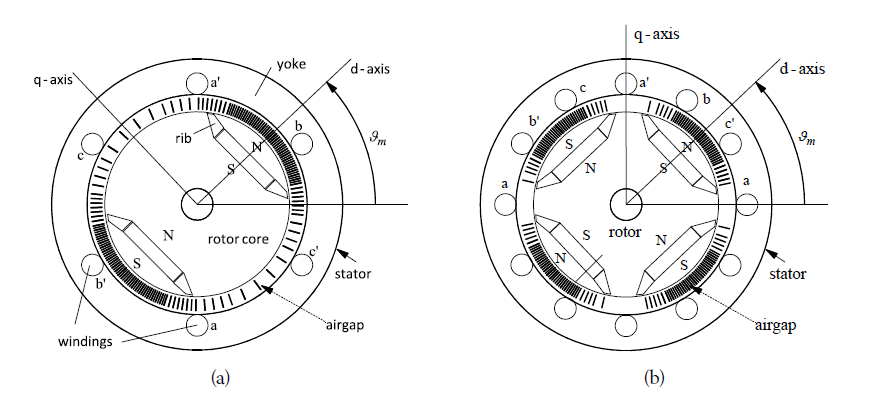
\includegraphics[width=1\linewidth]{immagini/immagini_motore/struttura_motore.png}
    \label{fig:Lez_10_5}
    \caption{Struttura del motore.}
\end{figure}

La distribuzione degli avvolgimenti di statore e la geometria dei magneti
permettono di ottenere flussi concatenati con il seguente andamento:

\begin{equation*}
\begin{aligned}
    &\lambda_{a,mg}=\Lambda_{mg}cos(\theta_{me})\\
     &\lambda_{b,mg}=\Lambda_{mg}cos(\theta_{me}-\frac{2}{3}\pi)\\
     &\lambda_{c,mg}=\Lambda_{mg}cos(\theta_{me}-\frac{4}{3}\pi)
    \end{aligned}\\
\end{equation*}
dove $\Lambda_{mg}$ rappresenta il massimo flusso concatenato dovuto al magnete permanente. Si può osservare come la terna di grandezze sia priva di componente omopolare; tale terna può quindi essere rappresentata tramite un unico vettore spaziale:

\begin{equation}
    \lambda_{mg}^s=\Lambda_{mg}e^{j\theta_{me}}
\end{equation}
 l’ apice $s$ indica che la grandezza è espressa secondo un sistema di riferimento stazionario,
 solidale con lo statore.  In tali motori la riluttanza lungo
l’ asse del loro campo magnetico (asse d) è maggiore rispetto a quella
secondo l’ asse ad essi ortogonale (asse q). L’ induzione magnetica è influenzata anche dal traferro e risulta dipendente anche della posizione del rotore. A differenza di altre tipologie di motore, le auto e mutue
induttanze non possono
essere considerate costanti, per la loro dipendenza dalla posizione del rotore e
dunque indirettamente anche dal tempo.\\
Le autoinduttanze del motore anisotropo si possono espriere nel modo seguente:
\begin{equation}
    \begin{aligned}
    &L_a=L_\sigma+L_0-L_2cos(2\theta_{me})\\
    &L_b=L_\sigma+L_0-L_2\cos{(2\theta_{me}-\frac{4}{3}\pi)}\\
    &L_c=L_\sigma+L_0-L_2\cos{(2\theta_{me}-\frac{2}{3}\pi})
    \end{aligned}
    \label{eq:inductances}
\end{equation}
dove indicando con $\Re_d$ ed $Re_q$ rispettivamente la riluttanza secondo l’asse d e
secondo l’asse q, e con N il numero “effttivo” di spire per fase, comprensivo di
ogni fattore necessario a correlare il numero di spire reali di un avvolgimento
distribuito con quello di un equivalente avvolgimento concentrato lungo ciascun
asse, si ha:

\begin{equation}
    L_0=N^2\frac{1/\Re_d+1/\Re_q}{2} \hspace{4mm} L_2=N^2\frac{1/\Re_d-1/\Re_q}{2} \hspace{4mm}
    \label{eq:double_L2}
\end{equation}
Come evidenziato dalla \ref{eq:inductances} le autoinduttanze si possono considerare somma
di due termini, uno sinusoidale a pulsazione doppia rispetto a quella elettromeccanica,
e l’altro costante. Quest’ultimo è formato a sua volta da due parti;
la prima, $L_0$, è legata ancora alla anisotropia della struttura, mentre la seconda,
$L_\sigma$ , rappresenta l’induttanza di dispersione ed è relativa al fluusso statorico che si
richiude in aria senza interessare il rotore.
Allo stesso modo, è possibile esprimere anche le mutue induttanze tra gli
avvolgimenti delle fasi statoriche, come segue:

\begin{equation}
\begin{aligned}
    & M_{ab}= \frac{1}{2}L_0-L_2\cos{\Big(2\theta_{me}-\frac{2\pi}{3}\Big)} \\
    & M_{bc}= \frac{1}{2}L_0-L_2\cos{(2\theta_{me})} \\
    & M_{ac}=-\frac{2}{2}L_0-L_2\cos{\Big(2\theta_{me}-\frac{4\pi}{3}\Big)}
\end{aligned}
\label{eq: equation4}
\end{equation}
dove $L_0$ ed $L_2$ rimangono  quelle definite dalle (\ref{eq: equation4}).\\
I flussi concatenati totali sono espressi dalla
\begin{equation}
\begin{aligned}
    & \lambda_a= L_ai_a+M_{ab}i_b+ M_{ac}i_c+ \lambda_{a,mg} \\
    & \lambda_a= L_bi_b+M_{ab}i_b+ M_{bc}i_c+ \lambda_{b,mg} \\
    & \lambda_a= L_ci_c+M_{ac}i_a+ M_{bc}i_b+ \lambda_{c,mg}
\end{aligned}
\label{eq: equation9}
\end{equation}
Le equazioni di bilancio delle tensioni sono:
\begin{equation}
\begin{aligned}
    & u_a= Ri_a+L_a\frac{di_a}{dt}+M_{ab}\frac{di_b}{dt}+M_{ac}\frac{di_c}{dt}+\frac{dL_a}{dt}i_a+\frac{dM_{ab}}{dt}i_b+\frac{dM_{ac}}{dt}i_c+e_a\\
    & u_b= Ri_b+L_b\frac{di_b}{dt}+M_{ab}\frac{di_a}{dt}+M_{bc}\frac{di_c}{dt}+\frac{dL_b}{dt}i_b+\frac{dM_{ab}}{dt}i_a+\frac{dM_{bc}}{dt}i_c+e_b \\
    & u_c= Ri_c+M_{ac}\frac{di_a}{dt}+M_{ab}\frac{di_a}{dt}+M_{bc}\frac{di_b}{dt}+\frac{dL_c}{dt}i_c+\frac{dM_{ac}}{dt}i_a+\frac{dM_{bc}}{dt}i_b+e_c \\
\end{aligned}
\label{eq: equation7}
\end{equation}
dove le forze contro-elettromotrici $e_a$,$e_b$, $e_c$ rimangono definite dalla
\begin{equation}
\begin{aligned}
    &e_a=\frac{d\lambda_{a,mg}}{dt}=-\Lambda_{mg}\omega_{me}sin(\theta_{me})\\
    &e_b=\frac{d\lambda_{b,mg}}{dt}=-\Lambda_{mg}\omega_{me}cos(\theta_{me}-\frac{\pi}{2}-\frac{2\pi}{3})\\
    &e_a=\frac{d\lambda_{a.mg}}{dt}=-\Lambda_{mg}\omega_{me}cos(\theta_{me}-\frac{\pi}{2}-\frac{4\pi}{3})\\
    \end{aligned}
\label{eq: equation5}
\end{equation}

Per comodità è utile esprimere le grandezze elettriche secondo il sistema di riferimento rotante. A tal scopo si impiega la seguente matrice di trasformazione di coordinate:

\begin{equation}
\mathbf{T_{abc/dq0}} = \frac{2}{3}
\begin{bmatrix}
    \cos (\vartheta_{me}) & \cos \left( \vartheta_{me} - \frac{2\pi}{3} \right) & \cos \left( \vartheta_{me} - \frac{4\pi}{3} \right) \\[6pt]
    -\sin (\vartheta_{me}) & -\sin \left( \vartheta_{me} - \frac{2\pi}{3} \right) & -\sin \left( \vartheta_{me} - \frac{4\pi}{3} \right) \\[6pt]
    \frac{1}{\sqrt{2}} & \frac{1}{\sqrt{2}} & \frac{1}{\sqrt{2}}
\end{bmatrix}
\label{eq:trasformazione_park}
\end{equation}
Le equazioni elettriche riportate \ref{eq: equation7}) possono essere espresse in maniera più compatta utilizzando una formulazione vettoriale:

\begin{equation}
\bm{u}_{abc}=\bm{Ri}_{abc}+\frac{d(\bm{L}_{abc}\bm{i}_{abc})}{dt}+\bm{e}_{abc}
\label{eq:equation10}
\end{equation}
dove le componenti vettoriali valgono:
\begin{align*}
\boldsymbol{u}_{abc} &= \begin{bmatrix} u_a & u_b & u_c \end{bmatrix} \\
\boldsymbol{i}_{abc} &= \begin{bmatrix} i_a & i_b & i_c \end{bmatrix} \\
\boldsymbol{e}_{abc} &= \begin{bmatrix} e_a & e_b & e_c \end{bmatrix}
\end{align*}
 le matrici $\bm{R}$ e $\bm{L_{abc}}$ sono definite come segue:
\begin{equation}
\bm{R} = 
\begin{bmatrix}
    R & 0 & 0 \\[6pt]
    0 & R & 0 \\[6pt]
    0 & 0 & R
\end{bmatrix}
\label{eq:trasformazione_park2}
\end{equation}

\begin{equation}
\bm{L}_{abc} = 
\begin{bmatrix}
    L_a & M_{ab} & M_{ac} \\[6pt]
    M_{ab} & L_b & M_{bc} \\[6pt]
    M_{ac} & M_{bc} & L_c
\end{bmatrix}
\label{eq:trasformazione_park3}
\end{equation}

Applicando alla (\ref{eq:equation10}) la trasformazione (\ref{eq:trasformazione_park}) si ottiene l’espressione matriciale
del bilancio delle tensioni nel sistema di riferimento sincrono, di seguito
riportata:
\begin{equation}
\mathbf{u}_{dq0}=\bm{Ri}_{dq0}+\bm{L}_{dq0}\frac{d\bm{i}_{dq0}}{dt}+\bm{e}_{abc}
\label{eq:electric_equa}
\end{equation}
dove
\begin{equation}
\begin{aligned}
\bm{u}_{dq0} &= [\, u_d \quad u_q \quad u_0 \;]' \\
\bm{i}_{dq0} &= [\, i_d \quad i_q \quad i_0 \,]
\end{aligned}
\label{eq:double_equa}
\end{equation}




ed inoltre, ricordando le (\ref{eq: equation5}):
\begin{equation}
    \bm{e}_{dq0}=[\,0\quad \omega_{me}\quad 0\,]'
\end{equation}
ed anche

\begin{align}
\bm{L}_{dq0} &=
\begin{bmatrix}
    L_d & 0 & 0 \\[6pt]
    0 & L_q & 0 \\[6pt]
    0 & 0 & L_\sigma
\end{bmatrix} \label{eq:trasformazione_park4} \\[12pt]
\bm{T} \frac{d\bm{T}^{-1}}{dt} &=
\begin{bmatrix}
    0 & -\omega_{me} & 0 \\[6pt]
    \omega_{me} & 0 & 0 \\[6pt]
    0 & 0 & 0
\end{bmatrix} \label{eq:trasformazione_park5}
\end{align}

come si può ricavare in maniera diretta applicando estesamente le formule di
Werner.\\
Le autoinduttanze $L_d$ e $L_q$ sono
legate ai termini $L_0$, $L_2$ ed $L_\sigma$ dalle relazioni:
\begin{equation}
L_d = L_\sigma + \frac{3}{2}(L_0 - L_2) \qquad L_q = L_\sigma + \frac{3}{2}(L_0 + L_2)    
\label{eq:double_L}
\end{equation}

Nei motori 
IPM la riluttanza del circuito magnetico associato all’asse $d$ è superiore a quella
relativa all’asse $q$ ne segue, dalle (\ref{eq:double_L2}) che $L_0$ ed $L_2$ siano entrambe positive, con
$L_0>L_2$; quanto scritto trova riscontro ovviamente anche nelle (\ref{eq:double_L}), ove
appare evidente che $L_q>L_d$. In particolare, il rapporto $L_q/L_d$ prende il nome
di rapporto di salienza e negli IPM può arrivarefino a 5.\\
Vale la pena di osservare che, in caso di rotore isotropo, verrebbe a mancare
il termine $L_2$. Si
preferisce l’impostazione attuale perché essa consente di arricchire di significato  fisico i vettori spaziali e, con essi, di dare una visione più intuitiva del principio
dell’orientamento di campo, che sta alla base degli azionamenti con motore
sincrono a magneti permanenti.\\
La relazione matriciale (\ref{eq:electric_equa}) può essere scritta tenendo conto delle (\ref{eq:double_equa})-(\ref{eq:trasformazione_park5})
per ciascuna delle sue tre componenti, ottenendo:

\begin{equation}
\begin{aligned}
    &u_d=Ri_d+L_d\frac{di_d}{dt}-\omega_{me}L_qi_q\\
    &u_q=Ri_q+L_q\frac{di_q}{dt}+\omega_{me}L_di_d+\omega_{me}\Lambda_{mg}\\
    &u_0=Ri_0+L_\sigma\frac{di_0}{dt}\\
    \end{aligned}
\label{eq: equation6}
\end{equation}
Le componenti della tensione secondo gli assi diretto ed in quadratura
hanno un’espressione sostanzialmente equivalente a quella ricavata per il motore
isotropo, quando in quest’ultima si sostituisca opportunamente all’induttanza
sincrona $L$ le induttanze sincrone d’asse diretto ed in quadratura.\\
Le espressioni (\ref{eq: equation6}) consentono di tracciare il bilancio energetico nel sistema
di riferimento sincrono, per ricavare un’espressione per la coppia meccanica
    sviluppata dal motore. In questo caso, si moltiplichino ambo i membri delle (\ref{eq: equation6}) rispettivamente per $i_ddt$, $i_qdtB$ e $i_odt$. Sommando membro a membro le tre
equazioni si ottiene:

\begin{equation}
\begin{aligned}
(u_d i_d + u_q i_q + u_0 i_0) dt &= R \left( i_d^2 + i_q^2 + i_0^2 \right) dt \\
&\quad + L_d i_d di_d + L_q i_q di_q + L_\sigma i_0 di_0 \\
&\quad + \omega_{me} \left( \Lambda_{mg} i_q + (L_d - L_q) i_d i_q \right) dt
\end{aligned}
\label{eq:bilancio_potenza}
\end{equation}

La coppia sviluppata dal motore risulta:
\begin{equation}
 \tau=\frac{3}{2}p\Lambda_{mg}i_q+\frac{3}{2}p(L_d-L_q)i_di_q
 \label{eq:equazione9}
\end{equation}

Rispetto al caso di motore isotropo si verifica la presenza di un ulteriore
termine, detto coppia di riluttanza.\\
Il contributo dovuto alla coppia di riluttanza accresce l’efficienza della conversione
elettromeccanica, intesa come rapporto tra coppia prodotta e modulo
(o valore massimo, a seconda del sistema di riferimento) della corrente di alimentazione.
I motori a magneti sepolti risultano dunque più economici di quelli a
magnete superficiale, perché è possibile impiegare meno materiale magnetico a
parità di coppia prodotta. La costruzione meccanica, che risulta intrinsecamente
robusta perché adatta a contrastare l’effetto della forza centrifuga sui magneti in
rotazione, e la possibilità di deflusare il motore in un range più esteso di quello
dei corrispondenti motori PMSM, rendono gli IPM adatti ad applicazioni ad
alte velocità ed alte prestazioni.\\
Nelle (\ref{eq: equation6}) appare anche l’equazione del bilancio della tensione $u_0$, che rappresenta
la tensione omopolare moltiplicata per un coefficiente di scala
$\sqrt{2}$. Tale
tensione insorge ad opera della corrente omopolare che normalmente è nulla
per l’assenza del filo neutro nella maggior parte dei motori sincroni a magneti
permanenti; come appare dalla (\ref{eq:equation10}) tale componente non partecipa alla creazione
della coppia e nello studio degli azionamenti per IPM verrà tralasciata.\\
In alcuni casi, come nelle moderne strategie di diagnosi dei guasti con adozione
automatica delle contromisure (fault-tolerant drives) vengono previsti
motori con il filo neutro, da collegare ad un quarto ramo dell’inverter che alimenta
il motore. Opportune tecniche di controllo provvedono poi ad isolare la
fase guasta e ad utilizzare il filo neutro come sua supplente; è nello studio di tali
tecniche avanzate che l’approccio generale presentato in questo paragrafo rivela
la sua utilità.\\
Dalle equazioni (\ref{eq: equation6}), (\ref{eq:equazione9}) e l’equazione che rappresenta il carico meccanico
si può infine tracciare lo schema a blocchi per il motore sincrono a magneti
permanenti di tipo anisotropo riportato nella Figura 2.
%______________________________________________________%

\section{Calcolo delle induttanza differenziali}
Le induttanze differenziali si possono ottenere calcolando le derivate parziali dei flussi:

\begin{equation}
\begin{dcases}
    \frac{d \lambda_d}{dt} = \frac{\partial \lambda_d}{\partial i_d} \frac{d i_d}{dt}+\frac{\partial \lambda_d}{\partial i_q} \frac{d i_q}{dt}+\frac{\partial \lambda_d}{\partial \theta_m} \frac{d \theta_m}{dt} \\[7pt] % <--- Aggiunge 15 punti di spazio
    \frac{d \lambda_q}{dt} = \frac{\partial \lambda_q}{\partial i_d} \frac{d i_d}{dt}+\frac{\partial \lambda_q}{\partial i_q} \frac{d i_q}{dt}+\frac{\partial \lambda_q}{\partial \theta_m} \frac{d \theta_m}{dt}
\end{dcases}
\end{equation}

Si può esprimere queste relazioni in maniera più compatta, usando il concetto di induttanze differenziali:

\begin{equation}
\begin{dcases}
    \frac{d \lambda_d}{dt} = l_d \frac{d i_d}{dt}+l_{dq} \frac{d i_q}{dt}+l_{d\theta} \frac{d \theta_m}{dt} \\[7pt] % <--- Aggiunge 15 punti di spazio
    \frac{d \lambda_q}{dt} = l_{qd} \frac{d i_d}{dt}+l_q \frac{d i_q}{dt}+l_{q\theta} \frac{d \theta_m}{dt}
\end{dcases}
\label{eq:induttanze_diff_elet}
\end{equation}


\cleardoublepage
\chapter{Set-up sperimentale}

\section{Procedura di misurazione}
Le mappe di flusso stimate esprimono il flusso magnetico in funzione delle componenti di corrente d-q e la posizione meccanica.\\
L'area di valutazione del modello è  un rettangolo nel piano $dq$. Tale rettangolo deve contenere tutte i punti di interesse per l'azionamento sotto test \cite{Armando}.\\
L'area viene così organizzata in una griglia equispaziata, individuata dai vettori di corrente della griglia:
\begin{equation}
\begin{cases}
    i_{d,k} = i_{d,\min} + k \cdot \Delta i_d & k = 1, 2, 3 \\
    i_{q,k'} = i_{q,\min} + k' \cdot \Delta i_q & k' = 1, 2, 3.
\end{cases}
\end{equation}

%\subsection{Procedura di misurazione}
%Bisogna anche tenere conto %del rischio di %smagnetizzazione.

\subsection{Set-up sperimentale}
Nel set-up sperimentale il motore di test (MUT) è accoppiato da un motore controllato in velocità. Tale motore trascina il motore di test imponendo una velocità di rotazione costante, l'articolo \cite{bojoi2024} propone una velocità pari a 1/3 della velocità nominale del motore di test.\\
Tenere una velocità elevata permette di ridurre l'effetto delle perdite nel ferro e nel magnete permanente durante il test.\\
Il MUT viene controllato in corrente. I valori di corrente di riferimento sono i punti della griglia di corrente sui quali si vuole stimare il flusso.\\
Dato che cge si adotta la convenzione degli a assi PM, il dominio dell'esplorazione del flusso copre il primo e il secondo quadrante del piano $i_{dq}$. Il dominio di corrente considerato è $i_d \in [-10\,\text{A}; 10\,\text{A}]$ e $i_q \in [0\,\text{A}; 10\,\text{A}]$.\\
Con riferimento al generico $k$-esimo punto di corrente $i_{dq,k}$, il processo di identificazione consiste di 3 fasi di misurazione:
\begin{itemize}
    \item primo impulso M1 (motore): il vettore di corrente è controllato in catena chiusa imponendo $\bm{i}_{dq}^{M1}=[i_{d,k}\ \ \ i_{q,k}]^T$;
    \item  impulso G (generatore): il segno di $i_q$ viene invertito per ottenere  $\bm{i}_{dq}^{G}=[i_{d,k}\ \ \ -i_{q,k}]^T$;
    \item seconfo impulso M2 (motore): il vettore di corrente è impostati nuovamente a
    $\bm{i}_{dq}^{M2}=[i_{d,k}\ \ \ i_{q,k}]^T$;
\end{itemize}
Una volta raggiunta la condizione a regime, le correnti di fase e le tensioni ai terminali del MUT vengono misurati, insieme alla posizione angolare per almeno una rotazione meccanica \cite{bojoi2024}.
\subsection{Simmetria delle condizioni di funzionamento come motore e come generatore}
Secondo la convenzione degli assi dei magneti permanenti, la componente fondamentale del flusso risulta simmetrica rispetto all'asse $d$:
\begin{equation}
\begin{cases}
    \lambda_d(i_d, i_q) = \lambda_d(i_d, -i_q) \\
    \lambda_q(i_d, i_q) = -\lambda_q(i_d, -i_q)
\end{cases}
\end{equation}

Alternando in sequenza il funzionamento della macchina motore da generatore a motore è possibile sfruttare tale simmetria per eliminare la tensione della resistenza di rotore. \\
Se il segno della corrente $i_q$ è invertito per ottenere il vettore simmetrico rispetto all'asse $d$, ogni componente armonico mantiene la stessa ampiezza, con fase specchiata. Perciò:

\begin{equation}
\begin{cases}
    \lambda_d(i_d, i_q,\theta) = \lambda_d(i_d, -i_q, -\theta) \\
    \lambda_q(i_d, i_q, \theta) = -\lambda_q(i_d, -i_q, -\theta)
\end{cases}
\end{equation}

Questa proprietà verrà sfruttata in seguito per stimare il flusso per eliminare la dipendenza dalla resistenza.


% COMPLETARE

\section{Procedure di misurazione}
Per minimizzare l'errore relativo causato dalle perdite nel ferro e dalle cadute di tensione parassite, è necessario che la FEM sia sufficientemente elevata rispetto ai disturbi. Pertanto, la velocità di rotazione meccanica deve essere elevata (ad esempio, pari a 1/3 della velocità nominale del MUT).\\
Inoltre, dato che la velocità è sostenuta, è fondamentale che la frequenza di campionamento del sensore di posizione sia sufficientemente elevata. Ciò è necessario per mappare accuratamente le forme d'onda della posizione in funzione della posizione meccanica $\theta_m$.\\



\subsection{Stima del flusso medio}
Prima di introdurre l'espressione usata per stimare il flusso medio.\\
Ai fini dell'identificazione del flusso concatenato, si considera l'equazione di tensione a regime permanente della macchina sincrona con riferimento a un determinato punto della griglia $(i_{d,k},i_{q,k})$ \cite{Armando}:

\begin{equation}
\left\{
\begin{aligned}
  v_{d,kk'} &= R_s \cdot i_{d,k} - \omega_e \cdot \lambda_{q,kk'} \\
  v_{q,kk'} &= R_s \cdot i_{q,k'} + \omega_e \cdot \lambda_{d,kk'}
\end{aligned}
\right.
\end{equation}

dove $\omega_e$ è la velocità elettrica e $R_s$ la resistenza di statore.
Il flusso concatenato può essere calcolato come segue:

\begin{equation}
\left\{
\begin{aligned}
  \lambda_{d,kk'} &= \frac{v_{q,kk'} - R_s \cdot i_{q,k'}}{\omega_e} \\
  \lambda_{q,kk'} &= -\left( \frac{v_{d,kk'} - R_s \cdot i_{d,k}}{\omega_e} \right)
\end{aligned}
\right.
\label{eq:eq_flux_exp}
\end{equation}

Dalla \ref{eq:eq_flux_exp} si può ricavare la seguente relazione:

\begin{equation}
\lambda_d = \frac{1}{2} \cdot \left( \frac{v_{q,1} + v_{q,3}}{2} + v_{q,2} \right) \cdot \frac{1}{\omega_e}
\end{equation}

\begin{equation}
\lambda_q = -\frac{1}{2} \cdot \left( \frac{v_{d,1} + v_{d,3}}{2} - v_{d,2} \right) \cdot \frac{1}{\omega_e}.
\label{fig:calcolo_flusso_media}
\end{equation}
La relazione \ref{fig:calcolo_flusso_media} verrà successivamente implementata nel codice.

\subsection{Temperatura del motore e gestione termica}
Dopo l'applicazione degli impulsi di corrente, necessario introdurre, un idle-time per permettere il motore di ritornare alla temperatura dell'ambiente (Figura \ref{fig:Grafico_impulsi}).\\
Durante l'applicazione degli impulsi la temperatura cresce con un andamento che può essere rappresentato come lineare. L'espressione \ref{fig:calcolo_flusso_media} permette di eliminare la dipendenza dalla temperatura.

\begin{figure}
\centering
    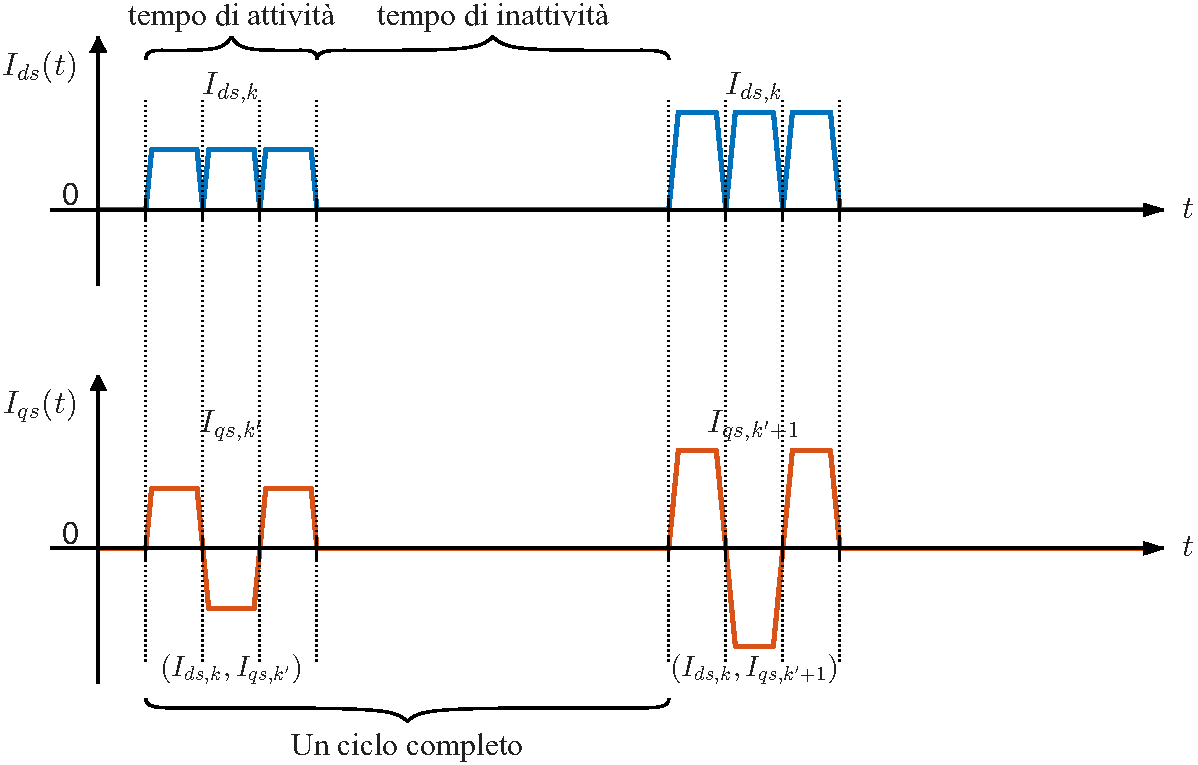
\includegraphics[height=7.5 cm]{immagini/grafici_matlab/Grafico_impulsi.pdf}
    \caption{Esempio della segquenza di impulsi $i_d$ e $i_q$.}
    \label{fig:Grafico_impulsi}
\end{figure}

\subsection{Stima del flusso in funzione della posizione elettrica}
\label{sec:stima_flusso}
Una volta raccolte le misure delle grandezze elettriche, si procede con la stima del flusso \cite{bojoi2024}.
Per comodità, si indicherà con $z_{x,k}^y$ un generico vettore di grandezze elettriche (tensione o corrente),$x$ si riferisce al sistema di riferimento $abc$, $\alpha\beta$ o $dq$, $y$ indica l'operazione $M_1$,$G$ o $M_2$ e $k$ l'indice del punto di misura nella griglia di corrente.
\begin{enumerate}
    \item Come primo passo, grandezze elettriche delle fasi di statore misurate $i^y_{abc,k}$, $v^y_{abc}$ devono essere riportate  secondo il sistema di riferimento $\alpha\beta$. Per far ciò i vettori di corrente e tensione vengono moltiplicati per la matrice di trasformazione.


\begin{equation}
\boldsymbol{z}_{\alpha\beta,k}^{y} = \frac{2}{3} \cdot 
\begin{bmatrix} 
1 & -\frac{1}{2} & -\frac{1}{2} \\ 
0 & -\frac{\sqrt{3}}{2} & \frac{\sqrt{3}}{2} 
\end{bmatrix} \cdot \boldsymbol{z}_{abc,k}^{y}
\label{eq:eq13}
\end{equation}

Basandosi sul (\ref{eq:eq13}), il flusso $\bf{\lambda}^y_{\alpha.\beta}$ può essere calcolato integrando la forza elettromotrice nel piano di riferimento $\alpha\beta$:

\begin{equation}
\boldsymbol{\lambda}_{\alpha\beta}^{y}(t) = \boldsymbol{\lambda}_{\alpha\beta}^{y}(t=0) + \int_{t_{0}}^{t_{0}+T} (\boldsymbol{v}_{\alpha\beta}^{y} - R_{s} \cdot \boldsymbol{i}_{\alpha\beta}^{y}) dt
\label{eq:integration_flux}
\end{equation}

dove $T$ corrisponde a una o più rivoluzioni meccaniche. La condizione iniziale del flusso può essere ottenuta tenendo conto che nel sistema $\alpha\beta$ in un periodo meccanico il flusso medio deve essere nullo:

\begin{equation}
\boldsymbol{\lambda}_{\alpha\beta}^{y}(t=0) = -mean \left( \int_{t_{0}}^{t_{0}+T} (v_{\alpha\beta}^{y} - R_{s} \cdot i_{\alpha\beta}^{y}) dt \right)
\end{equation}

\item \textbf{Interpolazione del flusso}: Dopo l'integrazione (\ref{eq:integration_flux}), le forme d'onda del flusso concatenato di M1,G e M2 sono determinate in funzione del tempo. A ogni istante temporale corrisponde un corrispettivo valore di posizione elettrica $\theta_e$. I vettori del flusso concatenato ottenuti per M1, G e M2 vengono ruotati dal sistema $\alpha\beta$ al sistema $dq$:

\begin{equation}
\boldsymbol{\lambda}_{dq,k}^y = 
\begin{bmatrix} 
\cos(\theta_e) & \sin(\theta_e) \\ 
-\sin(\theta_e) & \cos(\theta_e) 
\end{bmatrix} \cdot 
\boldsymbol{\lambda}_{\alpha\beta,k}^y \label{eq:matx_tr_dq}
\end{equation}

\item Calcolo delle mappe di flusso $dq\theta$: le stime di flusso durante le fasi M1, G e M2 sono ancora basate sull'integrazione (\ref{eq:integration_flux}), e così sensibili a errori dovuti al parametro resistivo. Per stimare le forme d'onda del flusso $\bm{\lambda}_{dq,k}^M(\bm{i}_{dq.k},\theta)$ e $\bm{\lambda}_{dq,k}^G(\bm{i}_{dq.k},\theta)$, includendo le armoniche spaziali e compensando la tensione resistiva, si applicano le seguenti espressioni:

\begin{subequations}
\label{eq:flussi_dq}
\begin{align}
    \lambda_d(\theta) &= \frac{\dfrac{\lambda_d^{M_1}(\theta_e) + \lambda_d^{M_2}(\theta_e)}{2} + \lambda_d^G(-\theta)}{2}  \\
    \lambda_q(\theta_e) &= \frac{\dfrac{\lambda_q^{M_1}(\theta_e) + \lambda_q^{M_2}(\theta_e)}{2} - \lambda_q^G(-\theta_e)}{2} \label{eq:estem_dq_l}
\end{align}
\end{subequations}

\end{enumerate}



\section{Stato dell'arte}
Esistono diversi metodi per stimare il flusso magnetico. Il modello magnetico del motore può essere estratto tramite delle simulazioni software ad elementi finiti (FEA).
Il metodo presentato in questa tesi permette di evitare l'utilizzo del software \cite{Zhao-Hong}.\\
Un problema che si riscontra nella stima del flusso è la variazione della resistenza a causa dell'aumento di temperatura.\\
Una possibile soluzione potrebbe essere quella di misurare la resistenza "on the fly", cioè prima della misurazione delle grandezze elettriche usate per stimare il flusso \cite{Gierczynski}. Tuttavia, questo metodo non permette di eliminare l'effetto dell'aumento di resistenza durante ciascuna degli stadi di misurazione (M1,G,M2).\\
Per quanto riguarda la misura di tensione, si può stimare la tensione a partire dal dutty-cycle, moltiplicando tale valore per la tensione di Bus. Dato che i tempi morti introducono un errore su questa stima, è necessario appliccare un algoritmo di compensazione il valore per ottenere il valore corretto \cite{Gierczynski}.\\


\cleardoublepage
\chapter{Analisi delle mappe di flusso del motore di test}
\raggedbottom
\section{Descrizione del motore di test}
Il motore di test è un motore IPM caratterizzato dai parametri riportati in Tabella \ref{tab:Tabella_parametri_motore}.\\
Dato che il motore possiede due coppie polari, i flussi $\lambda_d$ e $\lambda_q$ presentano una periodicità pari a 90 gradi meccanici. Perciò le mappe di flusso fornite presentano questo range angolare.\\

\begin{table} % Aggiunto [htbp] per il posizionamento
    \centering
    \footnotesize     
    \vspace{0.2cm}

    \renewcommand{\arraystretch}{1.3}
    
    % Definite 4 colonne invece di 3
    \begin{tabular}{
        >{\centering\arraybackslash}m{3 cm}
        >{\centering\arraybackslash}m{2 cm}        
        >{\centering\arraybackslash}m{2 cm} % Colonna aggiunta per pareggiare i conti
        >{\centering\arraybackslash}m{2.5 cm}
        }
        \arrayrulecolor{black}\toprule
        % Sistemata l'intestazione: rimossa la & di troppo
        \textbf{Parametro} & \textbf{Simbolo} & \textbf{Valore} & \textbf{Unità di misura} \\
        \arrayrulecolor{black}\midrule
        \textbf{Coppie polari} & $p$ & 2 & -\\ % p in math mode per il simbolo
        \arrayrulecolor{GRIG}\midrule
        \textbf{Resistenza di statore} &$R_s$ &2.726 & $\Omega$\\
        \arrayrulecolor{GRIG}\midrule
        \textbf{Induttanza di asse D} & $L_d$ & $20.5\cdot10^{-3}$ & $Hz$\\
        \arrayrulecolor{GRIG}\midrule
        \textbf{Induttanza di asse Q} & $L_q$ & 
        $114e\cdot10^{-3}$ & $Hz$\\
        \arrayrulecolor{GRIG}\midrule
        \textbf{Corrente nominale} & $I_n$ & $4.2$ & $A$\\
        \arrayrulecolor{GRIG}\midrule
        \textbf{Corrente nominale} & $I_N$ & $4.2$ & $A$\\
        \arrayrulecolor{GRIG}\bottomrule
        \textbf{Coppia nominale} & $\tau_N$ & $4.5$ & $Nm$\\
        \arrayrulecolor{GRIG}\bottomrule
        \textbf{Flusso magnete permanente} & $\lambda_{mg}$ & $0.22$ & $T$\\    
        \arrayrulecolor{GRIG}\bottomrule
        \textbf{Inerzia meccanica} & $J_m$ & $0.00094$ & $kgm^2$\\
        \arrayrulecolor{GRIG}\bottomrule
        \textbf{Attrito viscoso} & $B_m$ & $0.000155$ & $Nms/rad$\\
        \arrayrulecolor{GRIG}\bottomrule
        \textbf{Coppia di primo distacco} & $T_{ps}$ & $0.065$ & $Nms/rad$\\      
        \arrayrulecolor{black}\bottomrule
    \end{tabular}
    \caption{Parametri fisici del motore.}
    \label{tab:Tabella_parametri_motore}
\end{table}


\begin{table}[htbp] % Aggiunto [htbp] per il posizionamento
    \centering
    \footnotesize     
    \vspace{0.2cm}

    \renewcommand{\arraystretch}{1.3}
    
    % Definite 4 colonne invece di 3
    \begin{tabular}{
        >{\centering\arraybackslash}m{3 cm}
        >{\centering\arraybackslash}m{2 cm}        
        >{\centering\arraybackslash}m{2 cm} % Colonna aggiunta per pareggiare i conti
        >{\centering\arraybackslash}m{2.5 cm}
        }
        \arrayrulecolor{black}\toprule
        % Sistemata l'intestazione: rimossa la & di troppo
        \textbf{Parametro} &  \textbf{Valore} & \textbf{Unità di misura} \\
        \arrayrulecolor{black}\midrule
        \textbf{Risoluzione di posizione} & $2\pi/2^{16}$ & $rad$\\ % p in math mode per il simbolo
        \arrayrulecolor{GRIG}\midrule
        \textbf{Risoluzione di corrente} &0.001 & $A$\\
        \arrayrulecolor{GRIG}\midrule
        \textbf{Risoluzione di tensione} & 0.01 & $V$\\
        \arrayrulecolor{GRIG}\midrule
        \textbf{Frequenza di campionamento} & 10 & $KHz$\\
        \arrayrulecolor{black}\bottomrule
    \end{tabular}
    \caption{Parametri del sistema di misura.}
    \label{tab:Tabella_parametri_misura}
\end{table}

\section{Confronto dell'andamento del flusso con la velocità del rotore}
Per valutare l'effetto della velocità sul flusso magnetico concatenato, si sono confrontati gli andamenti del flusso all'aumentare della velocità.\\
Si può notare come, anche in questo caso, l'influenza della dipendenza dalla posizione nell'andamento due flussi sia simile. 

\begin{figure}
\centering
    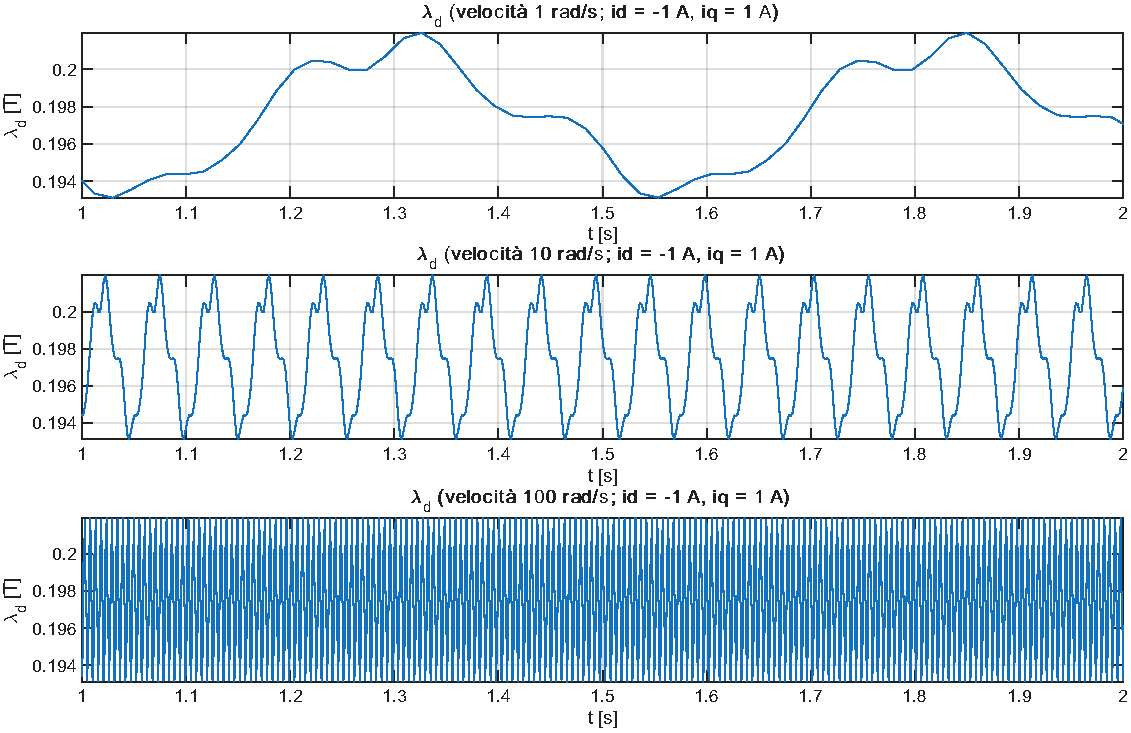
\includegraphics[height=7.5 cm]{immagini/flusso_concatenato/iq=m1/flusso_D_vs_velocità_iq_1.pdf}
    \caption{Andamento del flusso D al variare della velocità ($i_d$ = $i_q$ = -1 A).}
    \label{fig:flusso_D_vs_velocità_1}
\end{figure}

\begin{figure}
\centering
    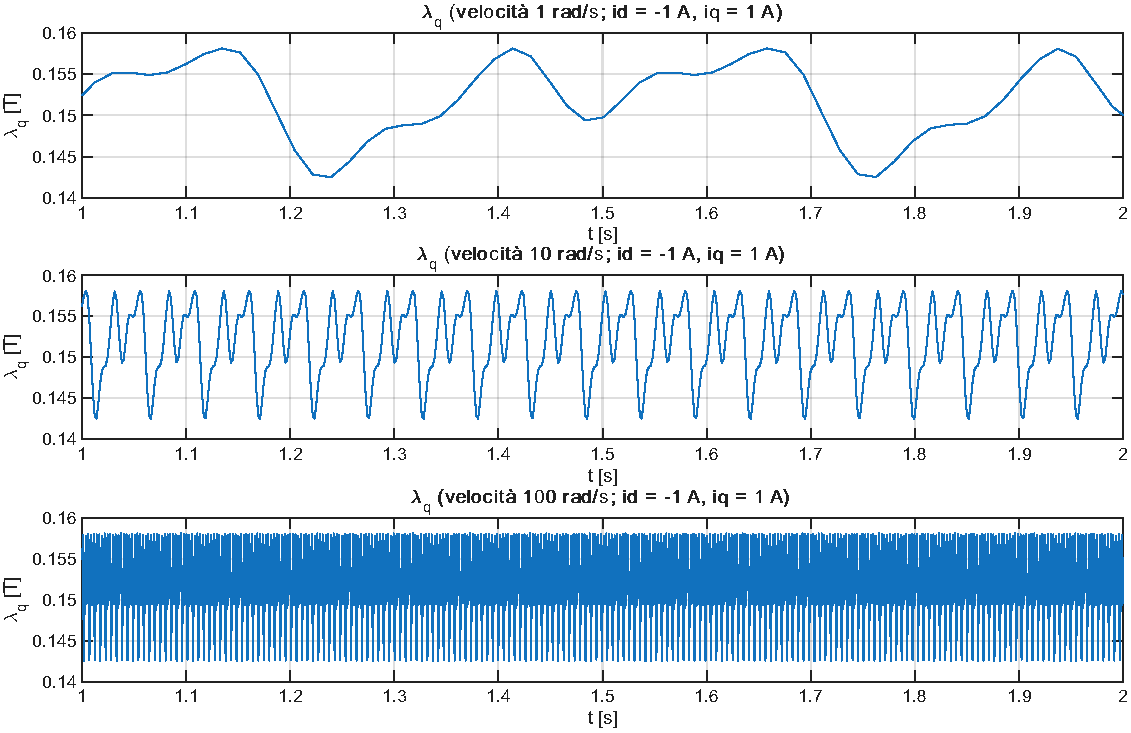
\includegraphics[height=7.5 cm]{immagini/flusso_concatenato/iq=m1/flusso_Q_vs_velocità_iq_1.pdf}
    \caption{Andamento del flusso Q al variare della velocità ($i_d$ = -1 A, $i_q$ = 1 A).}
    \label{fig:flusso_Q_vs_velocità_1}
\end{figure}







\section{Analisi delle armoniche del disturbo}
Si può notare come all'aumentare della velocità aumenti la frequenza dell'armonica principale del disturbo, mentre l'ampiezza rimane pressoché uguale. Non si riscontrano significative differenze tra le armoniche dei due flussi. 
Dall'analisi delle mappe di flusso si osserva come l'andamento del flusso si ripeta 3 volte in 90° meccanici, quindi 12 volte in una rotazione completa. Ciò permette di individuare dove è situata la fondamentale del disturbo sul flusso al variare della velocità meccanica, $\omega_m$ (1 rad/s):
\begin{equation}
    f_0=\frac{\omega_m\cdot 12}{2\pi} = 1.910 \ Hz
\end{equation}

 Conoscere questo dato diviene utile nel caso dell'aggiunta di un filtro passa alto per la rimozione del rumore a bassa frequenza; ciò permette di eliminare i disturbi senza attenuare o sfasare la prima armonica.


\begin{figure}
\centering
    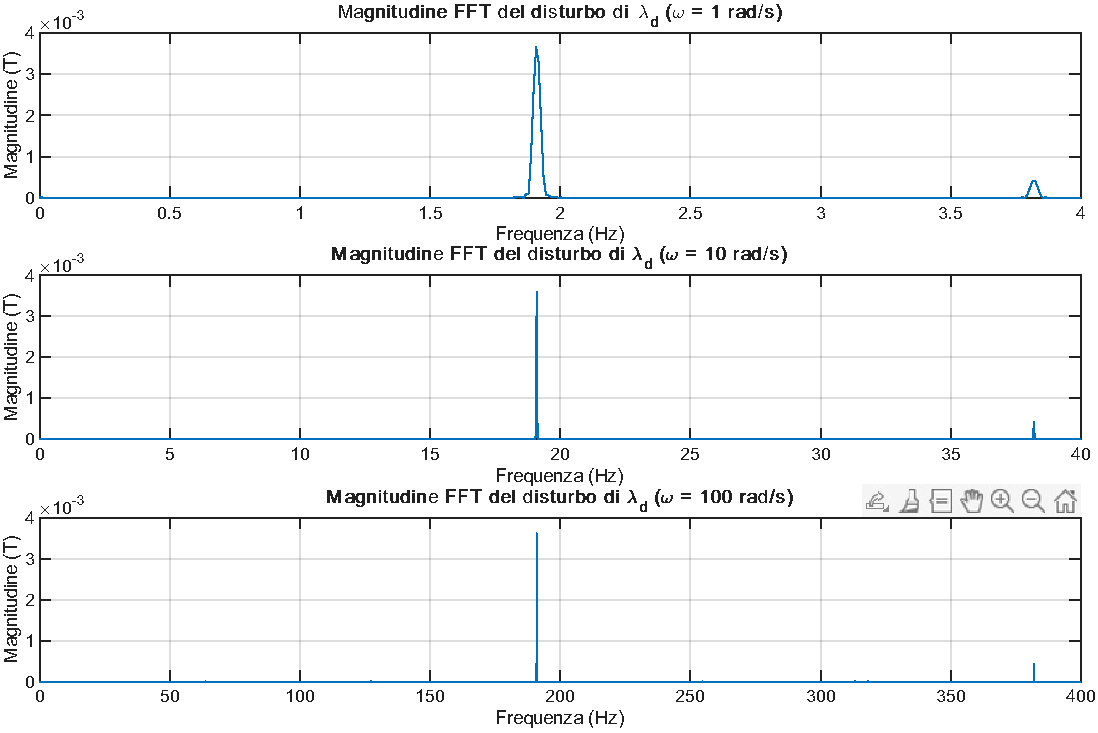
\includegraphics[height=7.5 cm]{immagini/flusso_concatenato/iq=m1/FFT_flusso_D_iq_1.pdf}
    \caption{FFT del flusso D al variare della velocità ($i_d$ = -1 A, $i_q$ = 1 A).}
    \label{fig:FFT_flusso_D_1}
\end{figure}

\begin{table}
    \centering
        
    \footnotesize
    
    \textbf{Analisi sul flusso $\lambda_d$}       
    
    \vspace{0.2cm}

    \renewcommand{\arraystretch}{1.3}
    
    \begin{tabular}{
        >{\centering\arraybackslash}m{3 cm}
        >{\centering\arraybackslash}m{2 cm}        
        >{\centering\arraybackslash}m{2.5 cm}
        }
\arrayrulecolor{black}\toprule
        \textbf{Velocità meccanica } &$\mathbf{Ampiezza}$ &$\mathbf{Frequenza}$ \\
       \text{[\,rad/s\,]} &\text{[\,V\,]} &\text{[\,Hz\,]} \\
            \arrayrulecolor{black}\midrule
            \textbf{1} & 0.00368 & 1.907 \\
            \arrayrulecolor{GRIG}\midrule
            \textbf{10}      & 0.00362 & 19.102 \\
            \arrayrulecolor{GRIG}\midrule
            \textbf{100}      & 0.00365 & 190.983 \\
        \arrayrulecolor{black}\bottomrule
    \end{tabular}
    \caption{Analisi sul flusso $\lambda_d$ con $i_d\ = \ -1\ A$ e $i_q\ = \ 1\ A$.}
    \label{tab:valore_forme_d'onda_flusso_D}   
\end{table}

Nel caso della FFT di $\lambda_q$ (Figura \ref{fig:FFT_flusso_Q_1}) si può notare come l'armonica con ampiezza maggiore sia collocata a una frequenza più alta rispetto a $\lambda_d$ (Figura \ref{fig:FFT_flusso_D_1}). I risultati numerici della FFT sono riportati in Figura \ref{tab:valore_forme_d'onda_flusso_D} e \ref{tab:valore_forme_d'onda_flusso_Q}.\\
Le forme d'onda del flusso vengono riportate nelle Figure \ref{fig:flusso_D_vs_velocità_1} e \ref{fig:flusso_Q_vs_velocità_1}. Ciò è dovuto alla forma particolare del segnale periodico, che presenta due picchi e non uno unico, come nel caso di $\lambda_d$. 





\begin{figure}
\centering
    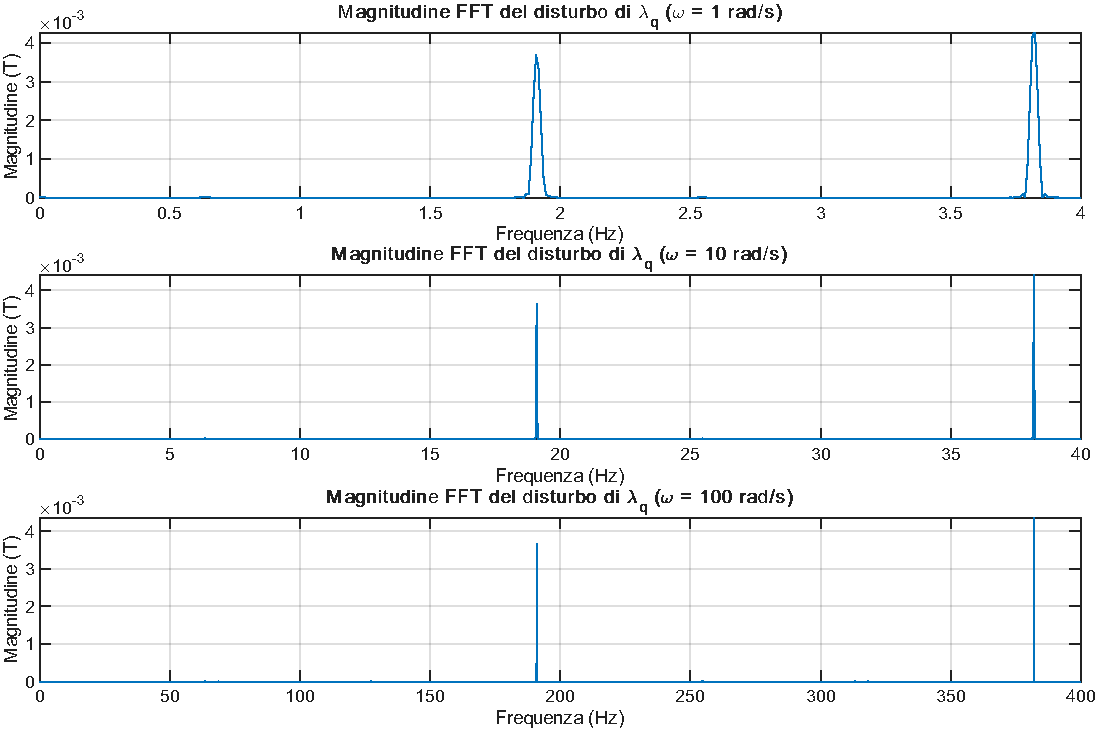
\includegraphics[height=7.5 cm]{immagini/flusso_concatenato/iq=m1/FFT_flusso_Q_iq_1.pdf}
    \caption{FFT del flusso Q al variare della velocità ($i_d$ = -1 A, $i_q$ = 1 A).}
    \label{fig:FFT_flusso_Q_1}
\end{figure}

\begin{table}
    \centering
        
    \footnotesize
    
    \textbf{Analisi sul flusso $\lambda_q$}       
    
    \vspace{0.2cm}

    \renewcommand{\arraystretch}{1.3}
    
    \begin{tabular}{
        >{\centering\arraybackslash}m{3 cm}
        >{\centering\arraybackslash}m{2 cm}        
        >{\centering\arraybackslash}m{2.5 cm}
        }
\arrayrulecolor{black}\toprule
        \textbf{Velocità meccanica } &$\mathbf{Ampiezza}$ &$\mathbf{Frequenza}$ \\
       \text{[\,rad/s\,]} &\text{[\,V\,]} &\text{[\,Hz\,]} \\
            \arrayrulecolor{black}\midrule
            \textbf{1} & 0.0045 & 3.815 \\
            \arrayrulecolor{GRIG}\midrule
            \textbf{10}      & 0.0046 & 38.193 \\
            \arrayrulecolor{GRIG}\midrule
            \textbf{100}      & 0.0047 & 381.97 \\
        \arrayrulecolor{black}\bottomrule
    \end{tabular}
    \caption{Analisi sul flusso $\lambda_q$ con $i_d\ = \ -1\ A$ e $i_q\ = \ 1\ A$.}
    \label{tab:valore_forme_d'onda_flusso_Q}   
\end{table}


\section{Valutazioni sull'impatto della posizione e corrente sul flusso}
Per valutare l'effettiva influenza delle correnti e della posizione meccanica, sono stati analizzati diversi grafici.\\
L'obiettivo dell'analisi è comprendere più a fondo la natura della mappa magnetica del motore e verificare l'impatto della dipendenza dalla posizione.




\subsection{Analisi del flusso $\lambda_{dq}$ espresso in funzione delle correnti.}
Si può notare anche come l'andamento del flusso $\lambda_d$ rimanga invariato invertendo il segno della corrente $i_q$ (Figure \ref{fig:Flusso_D_vs_Id_thetaVar} e \ref{fig:Flusso_D_vs_Id_thetaVar_iq_1}).\\
Fissando la corrente $i_q$, si può osservare come i flussi $\lambda_d$ e $\lambda_q$ abbiano un andamento monotono crescente (Figure \ref{fig:Flusso_D_vs_Id_thetaVar_iq_1} e \ref{fig:Flusso_Q_vs_Id_thetaVar_iq_1}).\\
Tale andamento crescente si riscontra anche con il flusso $\lambda_q$ fissando la corrente $i_d$ (Figura \ref{fig:Flusso_D_vs_Iq_thetaVar}). Al contrario, il flusso $\lambda_d$ con $i_d$ fissa non presenta questa tendenza.\\
Nel caso del cross-coupling si riscontra un maggiore effetto della variazione della posizione (Figure \ref{fig:Flusso_D_vs_Id_thetaVar_iq_1}, \ref{fig:Flusso_D_vs_Iq_thetaVar}  e \ref{fig:Flusso_Q_vs_Id_thetaVar}). Nell'accoppiamento diretto invece l'effetto è meno significativo e quasi ininfluente nel caso della Figura \ref{fig:Flusso_Q_vs_Iq_thetaVar}. 


\begin{figure}
\centering
    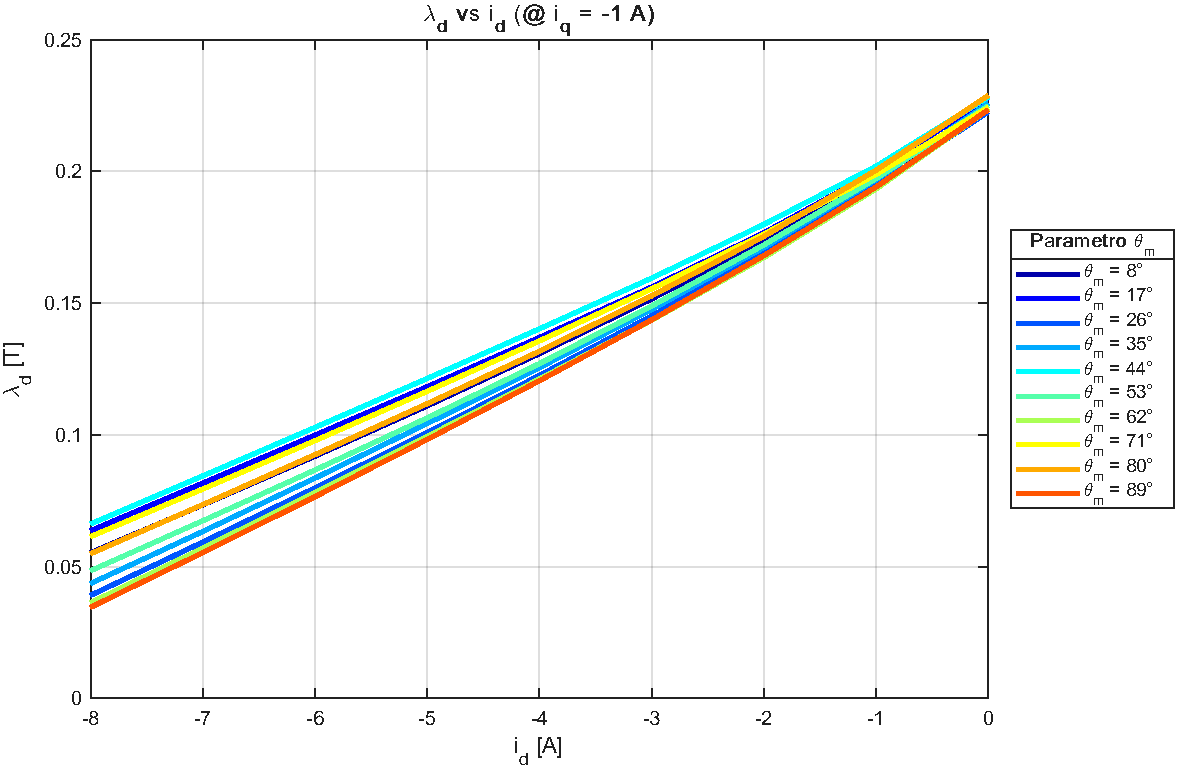
\includegraphics[height=7.5 cm]{immagini/flusso_concatenato/Flusso_D_vs_Id_thetaVar.pdf}
    \caption{Andamento del flusso D in funzione di $i_d$ a seconda della posizione @ $i_q$ = -1 A.}
    \label{fig:Flusso_D_vs_Id_thetaVar}
\end{figure}

\begin{figure}
\centering
    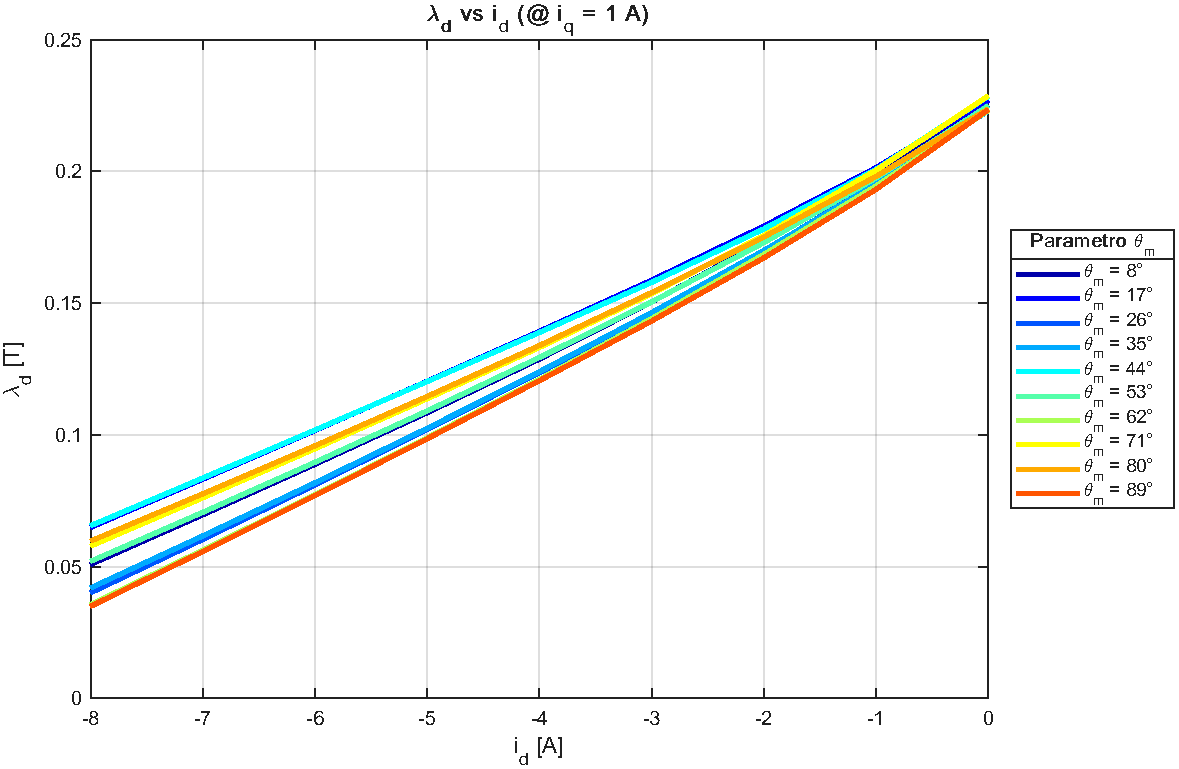
\includegraphics[height=7.5 cm]{immagini/flusso_concatenato/iq=m1/Flusso_D_vs_Id_thetaVar_iq_1.pdf}
    \caption{Andamento del flusso D in funzione di $i_d$ a seconda della posizione @ $i_q$ = 1 A.}
    \label{fig:Flusso_D_vs_Id_thetaVar_iq_1}
\end{figure}

\begin{figure}
\centering
    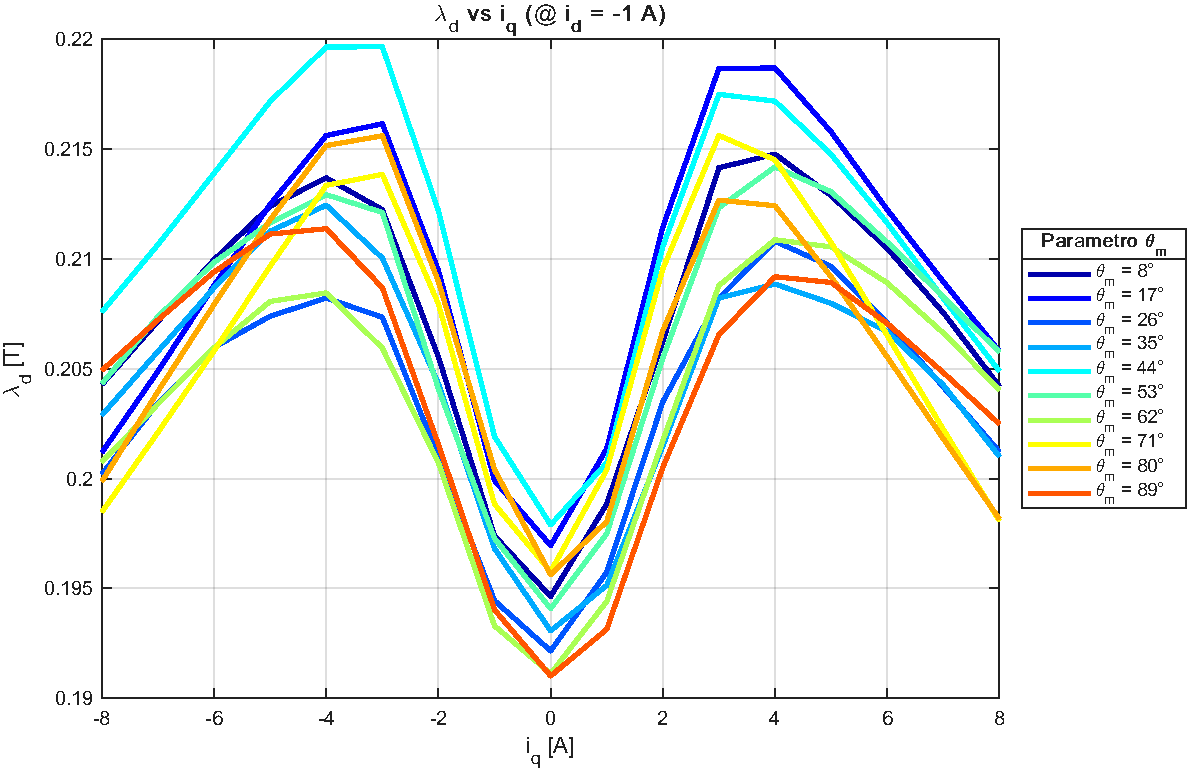
\includegraphics[height=7.5 cm]{immagini/flusso_concatenato/Flusso_D_vs_Iq_thetaVar.pdf}
    \caption{Andamento del flusso D in funzione di $i_q$ a seconda della posizione @ $i_d$ = -1 A.}
    \label{fig:Flusso_D_vs_Iq_thetaVar}
\end{figure}




\begin{figure}
\centering
    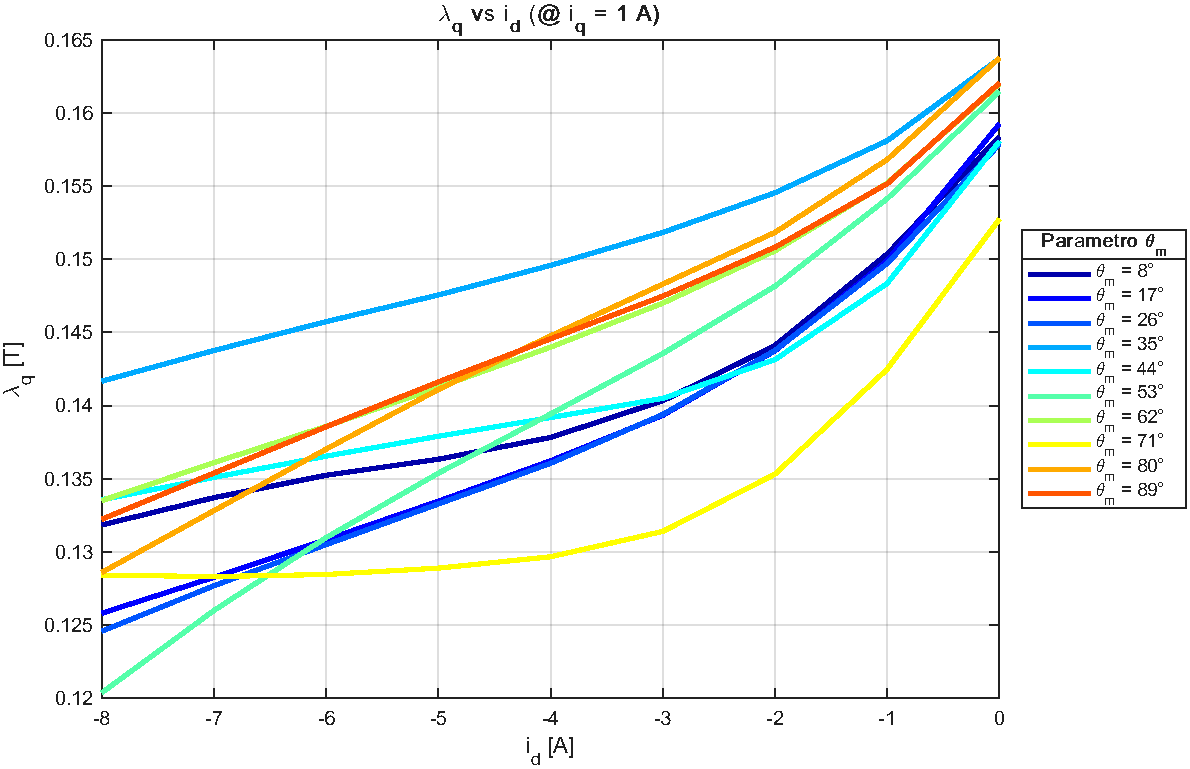
\includegraphics[height=7.5 cm]{immagini/flusso_concatenato/Flusso_Q_vs_Id_thetaVar.pdf}
    \caption{Andamento del flusso Q in funzione di $i_d$ a seconda della posizione @ $i_q$ = -1 A.}
    \label{fig:Flusso_Q_vs_Id_thetaVar}
\end{figure}


\begin{figure}
\centering
    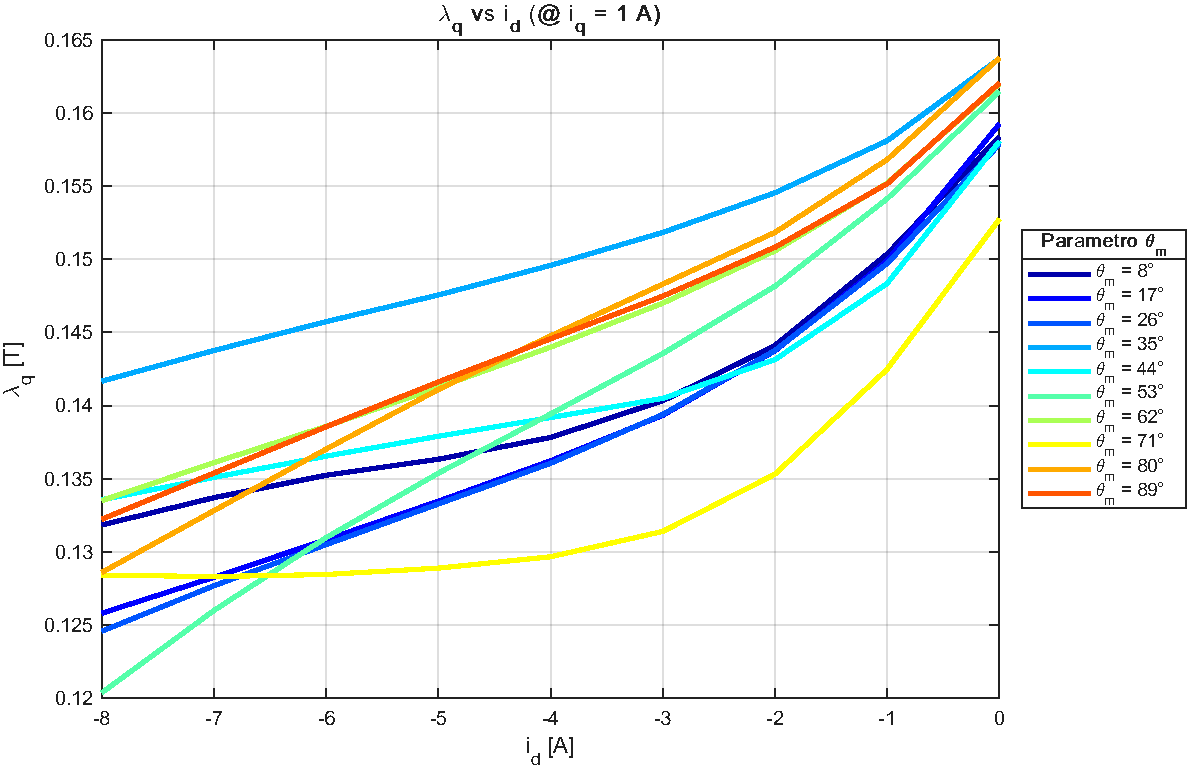
\includegraphics[height=7.5 cm]{immagini/flusso_concatenato/iq=m1/Flusso_Q_vs_Id_thetaVar_iq_1.pdf}
    \caption{Andamento del flusso Q in funzione di $i_d$ a seconda della posizione @ $i_q$ = 1 A.}
    \label{fig:Flusso_Q_vs_Id_thetaVar_iq_1}
\end{figure}

\begin{figure}
\centering
    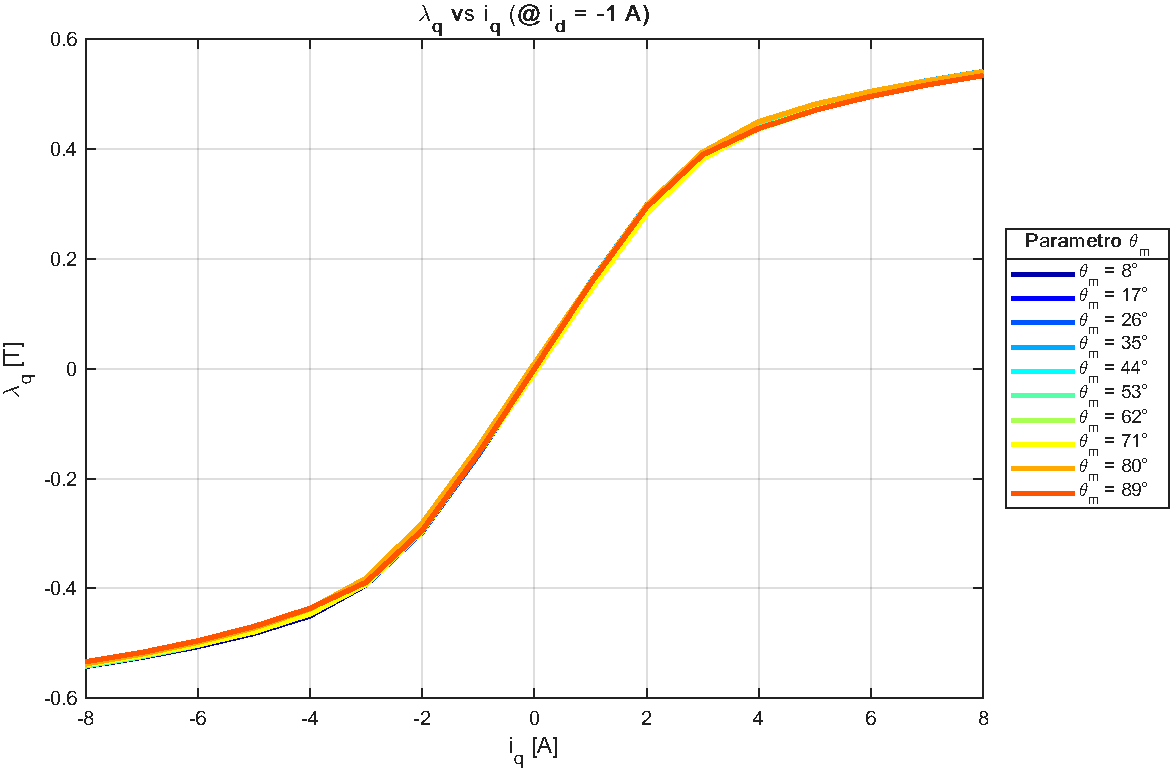
\includegraphics[height=7.5 cm]{immagini/flusso_concatenato/Flusso_Q_vs_Iq_thetaVar.pdf}
    \caption{Andamento del flusso Q in funzione di $i_q$ a seconda della posizione @ $i_d$ = -1 A.}
    \label{fig:Flusso_Q_vs_Iq_thetaVar}
\end{figure}

\subsection{Analisi del flusso $\lambda_{dq}$ espresso in funzione della posizione.}
Successivamente sono riportati i grafici del flusso in funzione della posizione.
Si può notare come l'impatto della posizione sul valore del flusso dipenda dall'intensità della corrente.\\ L'inversione di $i_q$ non influenza il flusso $\lambda_d$, rispetto al quale presenta un comportamento simmetrico (Figure  \ref{fig:Flusso_D_vs_theta_IdVar} e \ref{fig:Flusso_D_vs_theta_IdVar_iq_1}).\\
Al contrario, il legame tra la corrente $i_q$ e il flusso $\lambda_q$ è di tipo antisimmetrico: invertendo il segno della corrente, si inverte il segno del flusso (Figure  \ref{fig:Flusso_Q_vs_theta_IdVar} e \ref{fig:Flusso_Q_vs_theta_IdVar_iq_1}).\\
Nelle Figure \ref{fig:Flusso_D_vs_theta_IdVar} e \ref{fig:Flusso_D_vs_theta_IdVar_iq_1} si può anche notare come l'ampiezza del flusso magnetico $\lambda_d$ e il valore medio tenda ad incrementare all'aumentare del parametro di corrente $i_d$.
Nella Figura \ref{fig:Flusso_D_vs_theta_IqVar2}, si osserva come l'ampiezza picco-picco del disturbo aumenti all'aumentare della corrente $i_d$. Anche in questo caso è confermato che il disturbo influenza maggiormente il cross-coupling.\\
Nella Figura \ref{fig:Flusso_Q_vs_theta_IdVar}, si osserva come l'ampiezza picco-picco del disturbo sia ridotta e rimanga pressochè inalterata al variare della corrente $i_q$.
Confrontando la Figura \ref{fig:Flusso_Q_vs_theta_IdVar} e la Figura \ref{fig:Flusso_Q_vs_theta_IdVar_iq_1} si può notare l'antisimmetricità del flusso $\lambda_q$ rispetto alla corrente $i_q$.\\
In Figura \ref{fig:Flusso_Q_vs_theta_IqVar} viene ripoertato l'andamento del flusso, fissando la corrente $i_d$.

\begin{figure}
\centering
    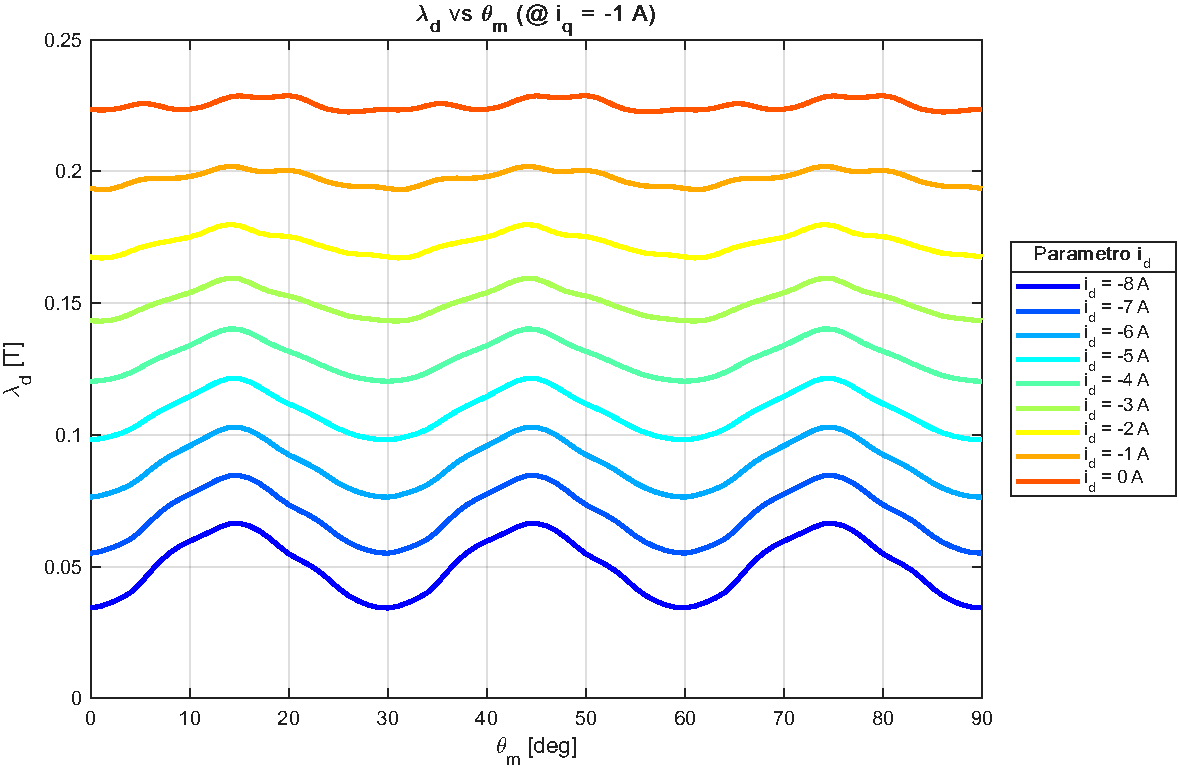
\includegraphics[height=7.5 cm]{immagini/flusso_concatenato/Flusso_D_vs_theta_IdVar.pdf}
    \caption{Andamento del flusso D in funzione di $\theta_m$ a seconda della posizione @ $i_q$ = -1 A. Massima ampiezza picco-picco = 0.0375 T. Massima deviazione standard (disturbo) = 0.0132 T.}
    \label{fig:Flusso_D_vs_theta_IdVar}
\end{figure}



\begin{figure}
\centering
    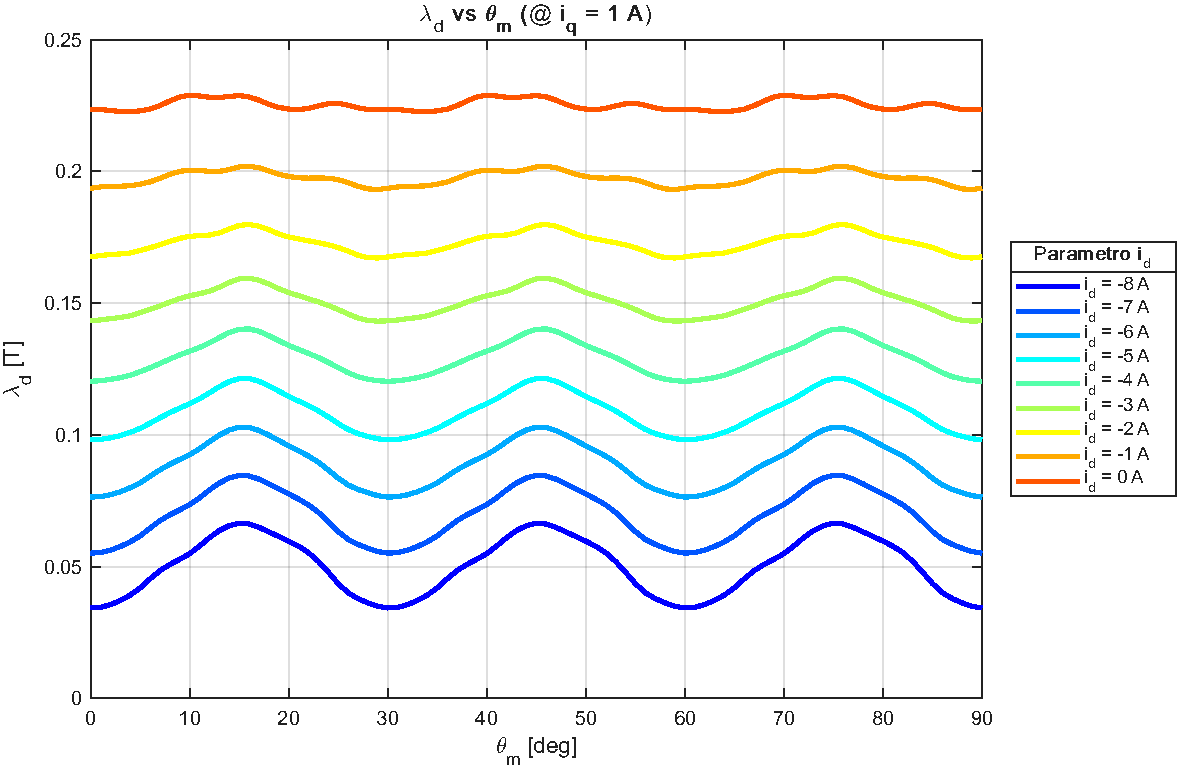
\includegraphics[height=7.5 cm]{immagini/flusso_concatenato/iq=m1/Flusso_D_vs_theta_IdVar_iq_1.pdf}
    \caption{Andamento del flusso D in funzione di $\theta_m$ a seconda della posizione @ $i_q$ = 1 A. Massima ampiezza picco-picco = 0.0375 T. Massima deviazione standard (disturbo) = 0.0132 T.}
    \label{fig:Flusso_D_vs_theta_IdVar_iq_1}
\end{figure}

\begin{figure}
\centering
    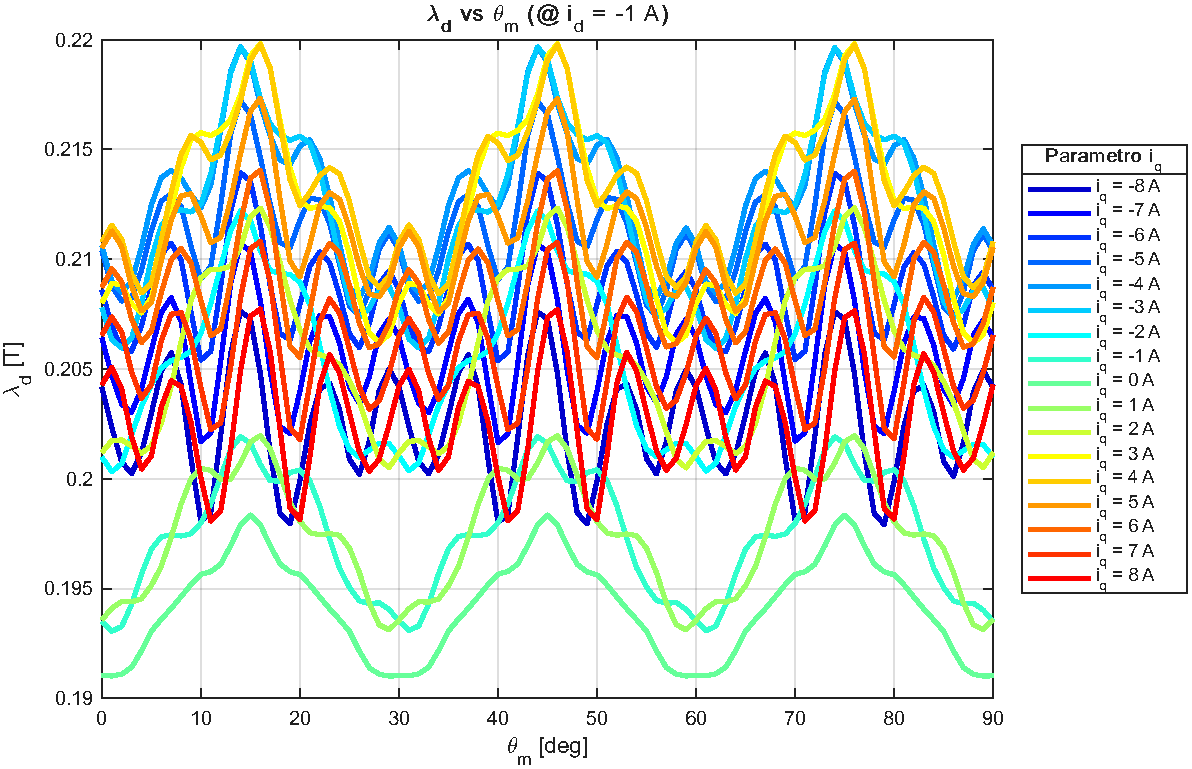
\includegraphics[height=7.5 cm]{immagini/flusso_concatenato/Flusso_D_vs_theta_IqVar.pdf}
    \caption{Andamento del flusso D in funzione di $\theta_m$ a seconda della posizione @ $i_d$ = -1 A. Massima ampiezza picco-picco = 0.0143 T. Massima deviazione standard (disturbo) = 0.0041 T. }
    \label{fig:Flusso_D_vs_theta_IqVar2}
\end{figure}



\begin{figure}
\centering
    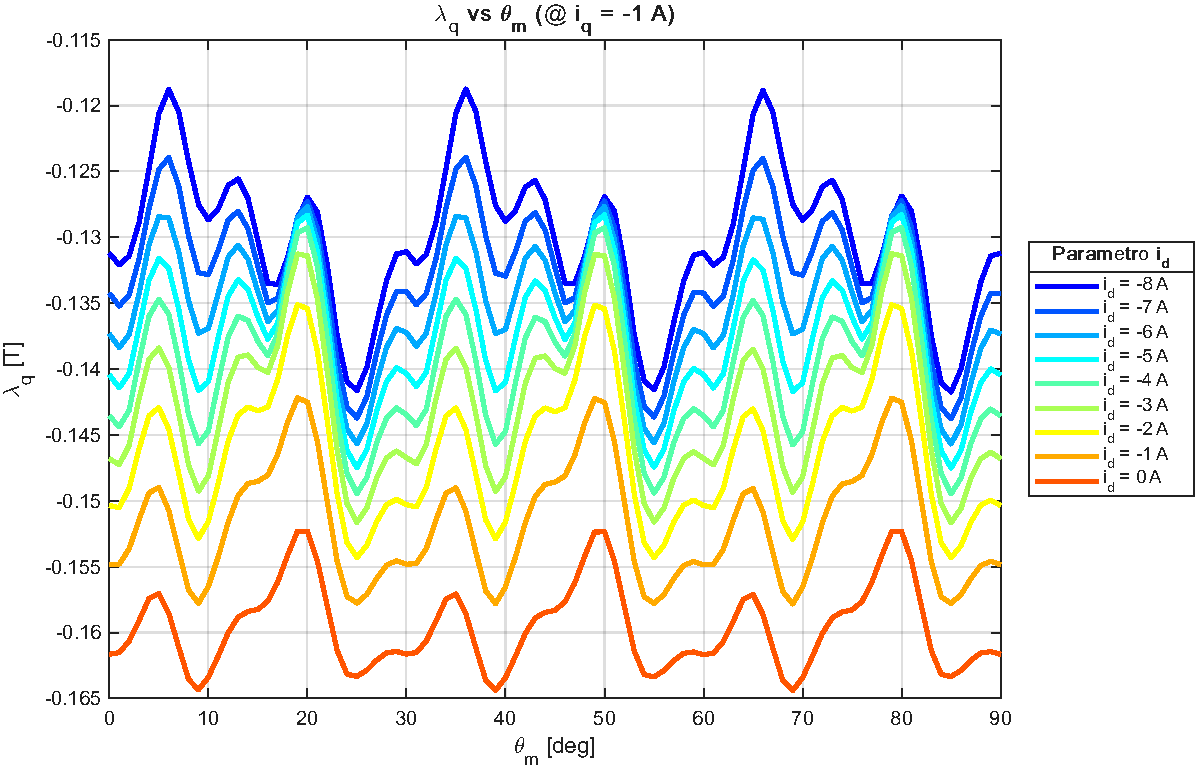
\includegraphics[height=7.5 cm]{immagini/flusso_concatenato/Flusso_Q_vs_theta_IdVar.pdf}
    \caption{Andamento del flusso Q in funzione di $\theta_m$ a seconda della posizione @ $i_q$ = -1 A. Massima ampiezza picco-picco = 0.0345 T. Massima deviazione standard (disturbo) = 0.0087 T.}
    \label{fig:Flusso_Q_vs_theta_IdVar}
\end{figure}


\begin{figure}
\centering
    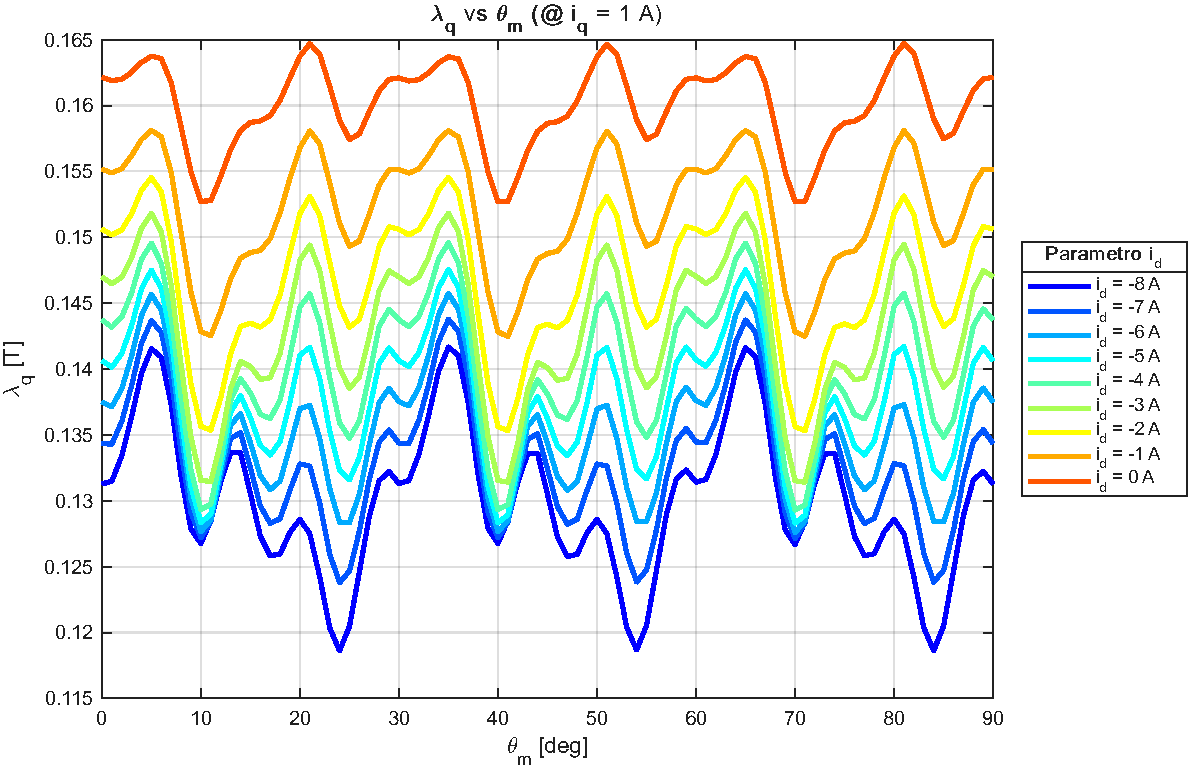
\includegraphics[height=7.5 cm]{immagini/flusso_concatenato/iq=m1/Flusso_Q_vs_theta_IdVar_iq_1.pdf}
    \caption{Andamento del flusso Q in funzione di $\theta_m$ a seconda della posizione @ $i_q$ = 1 A. Massima ampiezza picco-picco = 0.0344 T. Massima deviazione standard (disturbo) = 0.0087 T.}
    \label{fig:Flusso_Q_vs_theta_IdVar_iq_1}
\end{figure}




\begin{figure}
\centering
    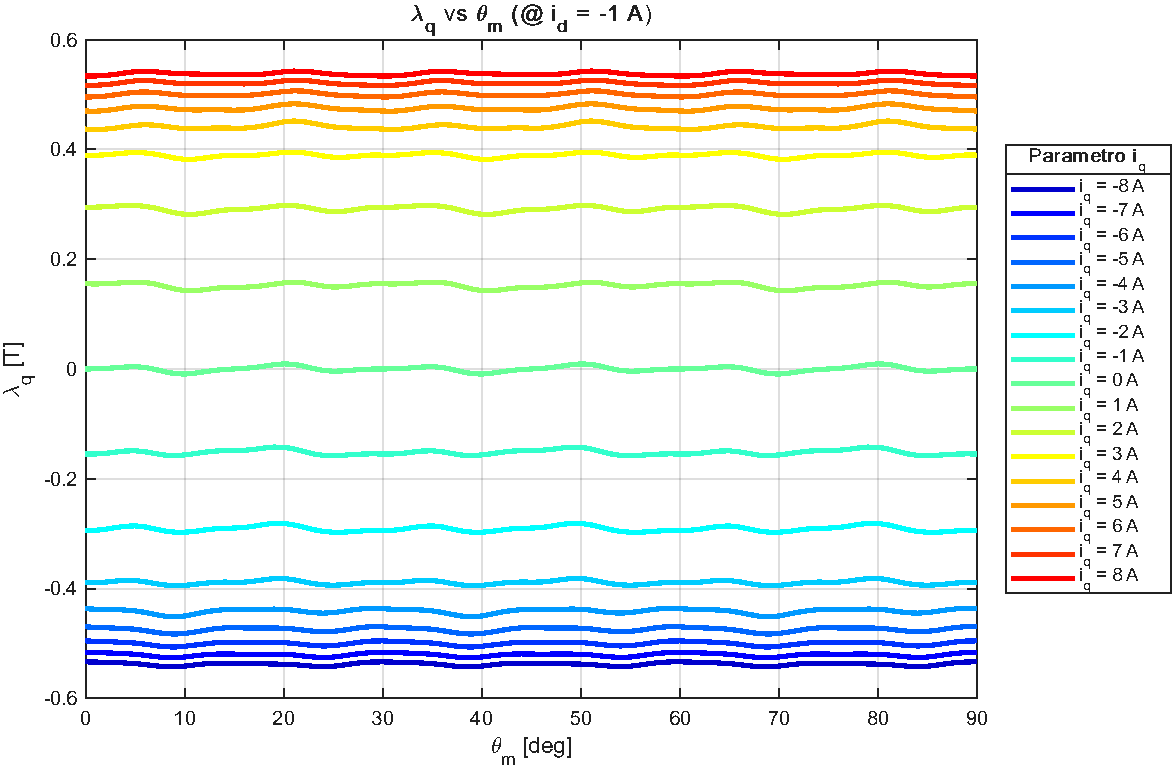
\includegraphics[height=7.5 cm]{immagini/flusso_concatenato/Flusso_Q_vs_theta_IqVar.pdf}
    \caption{Andamento del flusso Q in funzione di $\theta_m$ a seconda della posizione @ $i_d$ = -1 A. Massima ampiezza picco-picco = 0.0199 T. Massima deviazione standard (disturbo) = 0.0051 T.}
    \label{fig:Flusso_Q_vs_theta_IqVar}
\end{figure}



\subsection{Analisi della fcem}
Si riporta poi l'andamento della fcem al variare della velocità meccanica. Si può notare come all'aumentare della velocità aumenti l'ampiezza del disturbo sulla fcem e la frequenza del segnale (Figure \ref{fig:fcem_D_vs_velocità} e \ref{fig:fcem_Q_vs_velocità}). Questo andamento è confermato anche dai dati riportati nelle Tabelle \ref{tab:valore_forme_d'onda_fcem_D} e \ref{tab:valore_forme_d'onda_fcem_Q}. Questo è un comportamento atteso, dato il legame che lega la velocità di rotazione alla fcem:
\begin{equation}
 e_{dq}=\omega_{e}\cdot \lambda_{dq}
\end{equation}
\begin{figure}
\centering
    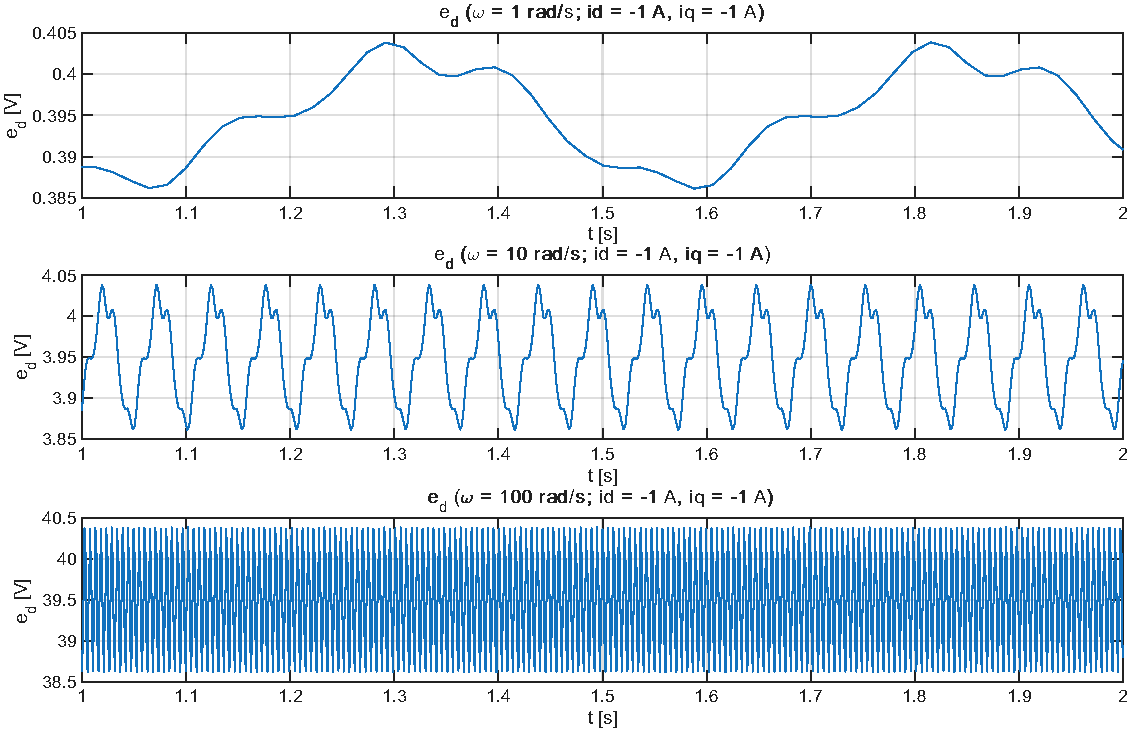
\includegraphics[height=7.5 cm]{immagini/fcem/fcem_D_vs_velocità.pdf}
    \caption{Andamento della tensione fcem D al variare della velocità ($i_d$ = -1 A, $i_q$ = -1 A).}
    \label{fig:fcem_D_vs_velocità}
\end{figure}



\begin{figure}
\centering
    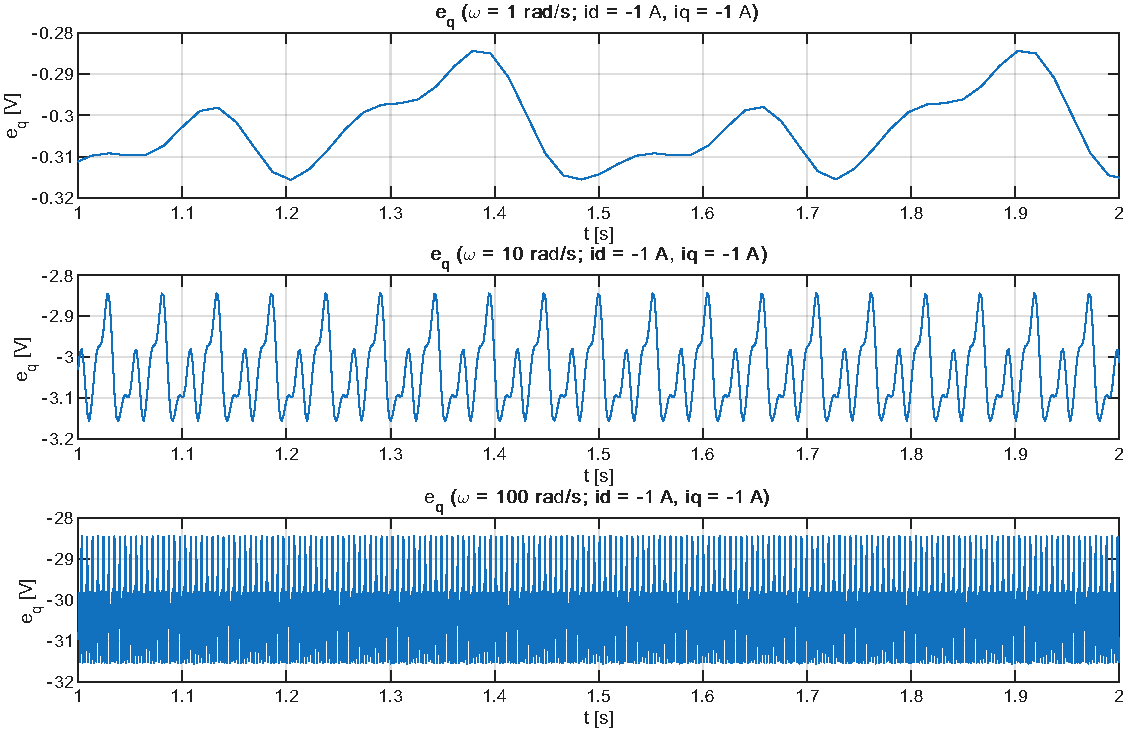
\includegraphics[height=7.5 cm]{immagini/fcem/fcem_Q_vs_velocità.pdf}
    \caption{Andamento della tensione fcem Q al variare della velocità ($i_d$ = -1 A, $i_q$ = 1 A).}
    \label{fig:fcem_Q_vs_velocità}
\end{figure}



\begin{figure}
\centering
    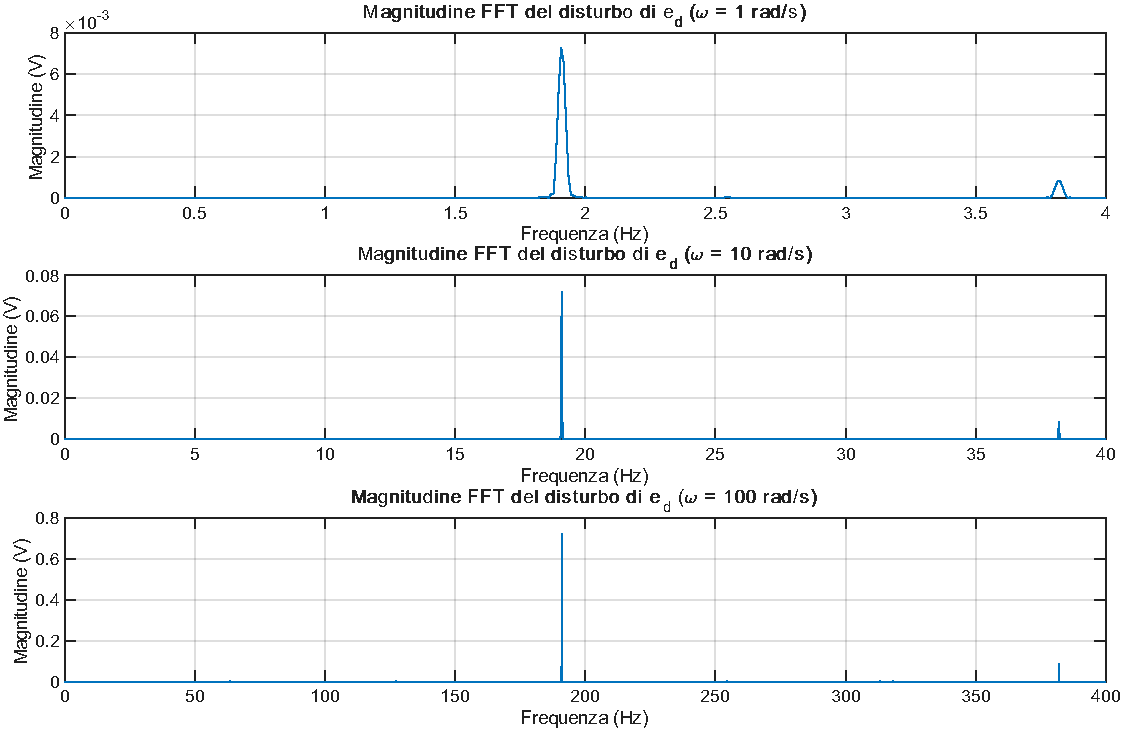
\includegraphics[height=7.5 cm]{immagini/fcem/FFT_fcem_D.pdf}
    \caption{FFT della fcem D al variare della velocità ($i_d$ = $i_q$ = -1 A).}
    \label{fig:FFT_fcem_D}
\end{figure}

\begin{figure}
\centering
    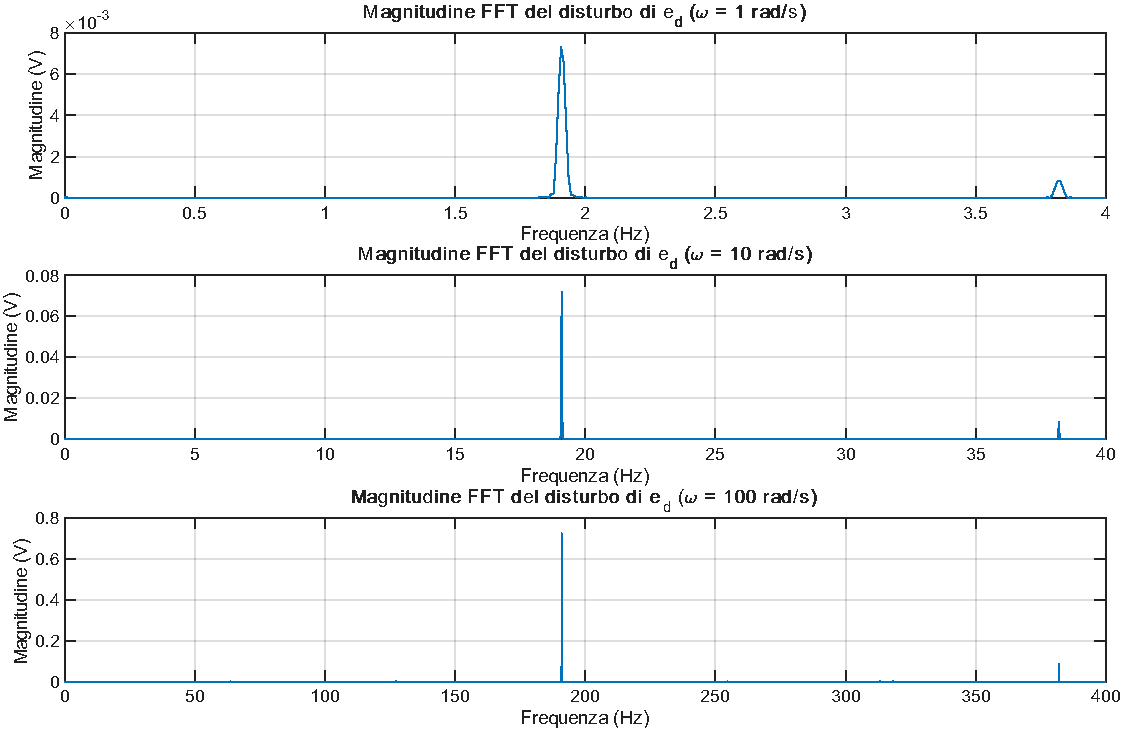
\includegraphics[height=7.5 cm]{immagini/fcem/iq=m1/FFT_fcem_D_iq_1.pdf}
    \caption{FFT della componente d della fcem al variare della velocità ($i_d$ = -1 A, $i_q$ = 1 A).}
    \label{FFT_fcem_D_iq_1}
\end{figure}

\begin{table}
    \centering
        
    \footnotesize
    
    \textbf{Analisi sulla fcem $e_d$}        
    
    \vspace{0.2cm}

    \renewcommand{\arraystretch}{1.3}
    
    \begin{tabular}{
        >{\centering\arraybackslash}m{3 cm}
        >{\centering\arraybackslash}m{2 cm}        
        >{\centering\arraybackslash}m{2.5 cm}
        }
\arrayrulecolor{black}\toprule
        \textbf{Velocità meccanica } &$\mathbf{Ampiezza}$ &$\mathbf{Frequenza}$ \\
       \text{[\,rad/s\,]} &\text{[\,T\,]} &\text{[\,Hz\,]} \\
            \arrayrulecolor{black}\midrule
            \textbf{1} & 0.0073 & 1.9074 \\
            \arrayrulecolor{GRIG}\midrule
            \textbf{10}      & 0.0718 & 19.102 \\
            \arrayrulecolor{GRIG}\midrule
            \textbf{100}      & 0.723 & 190.983 \\
        \arrayrulecolor{black}\bottomrule
    \end{tabular}
    \caption{Analisi sulla fcem $e_d$ con $i_d\ = \ -1\ A$ e $i_q\ = \ 1\ A$.}
    \label{tab:valore_forme_d'onda_fcem_D}  
\end{table}


La distribuzione in frequenza della fcem rispecchia la distribuzione trovata per la FFT di $\lambda_d$ e $\lambda_q$.



\begin{table}
    \centering
        
    \footnotesize
    
    \textbf{Analisi sulla fcem $e_q$}       
    
    \vspace{0.2cm}

    \renewcommand{\arraystretch}{1.3}
    
    \begin{tabular}{
        >{\centering\arraybackslash}m{3 cm}
        >{\centering\arraybackslash}m{2 cm}        
        >{\centering\arraybackslash}m{2.5 cm}
        }
\arrayrulecolor{black}\toprule
        \textbf{Velocità meccanica } &$\mathbf{Ampiezza}$ &$\mathbf{Frequenza}$ \\
       \text{[\,rad/s\,]} &\text{[\,T\,]} &\text{[\,Hz\,]} \\
            \arrayrulecolor{black}\midrule
            \textbf{1} & 0.009 & 3.8147 \\
            \arrayrulecolor{GRIG}\midrule
            \textbf{10} &   0.0911  & 38.195 \\
            \arrayrulecolor{GRIG}\midrule
            \textbf{100}      & 0.9493 & 381.98 \\
        \arrayrulecolor{black}\bottomrule
    \end{tabular}
    \caption{Analisi sulla fcem $e_q$ con $i_d\ = \ -1\ A$ e $i_q\ = \ 1\ A$.}
    \label{tab:valore_forme_d'onda_fcem_Q} 
\end{table}

\section{Stima della curva MTPA}
Si può poi analizzare l'andamento del flusso lungo la curva dei punti MTPA.
Tali punti sono di particolare interesse perchè la curva MTPA comprende tutti quei punti di corrente che sono coinvolti in tale controllo.\\
Per tracciare tale curva, si è eliminata la dipendenza della posizione, mediando per ogni coppia di correnti il flusso magnetico su un giro meccanico. L'obiettivo infatti non è quello di ottenere una stima precisa della curva MTPA, ma un valore indicativo per poi selezionare dei punti di corrente di interesse per l'analisi del flusso magnetico concatenato.\\
Per stimare la curva MTPA si utilizza una funzione di minimizzazione. \\
L'obiettivo è quello di ottenere a parità di corrente il valore massimo di coppia erogabile. Per far ciò si definisce come funzione di costo l'espressione della coppia con segno negativo:




\section{Analisi del flusso rispetto al punto nominale}
Si possono calcolare le coordinate del punto nominale della curva considerando il vincolo imposto dalla corrente nominale ($I_N = 4.2\,\mathrm{A}$).
Tale punto è individuato dall'intersezione tra la curva MTPA e la circonferenza di corrente avente come raggio la corrente nominale.
Si ottiene che le componenti di corrente nominale sono $i_d = -2.769$ A e $i_q = 3.158$ A. Il vincolo sulla corrente è rappresentato visivamente in Figura \ref{fig:Risultati_MTPA}.\\
Il profilo del flusso magnetico associato al punto di corrente nominale è riportato in Figura \ref{fig:Confronto_Flussi_PuntoTarget_0}
Al contrario del caso precedente, si nota una riduzione dell'ampiezza dell'oscillazione sul flusso all'aumentare della corrente.

\begin{figure}
\centering
    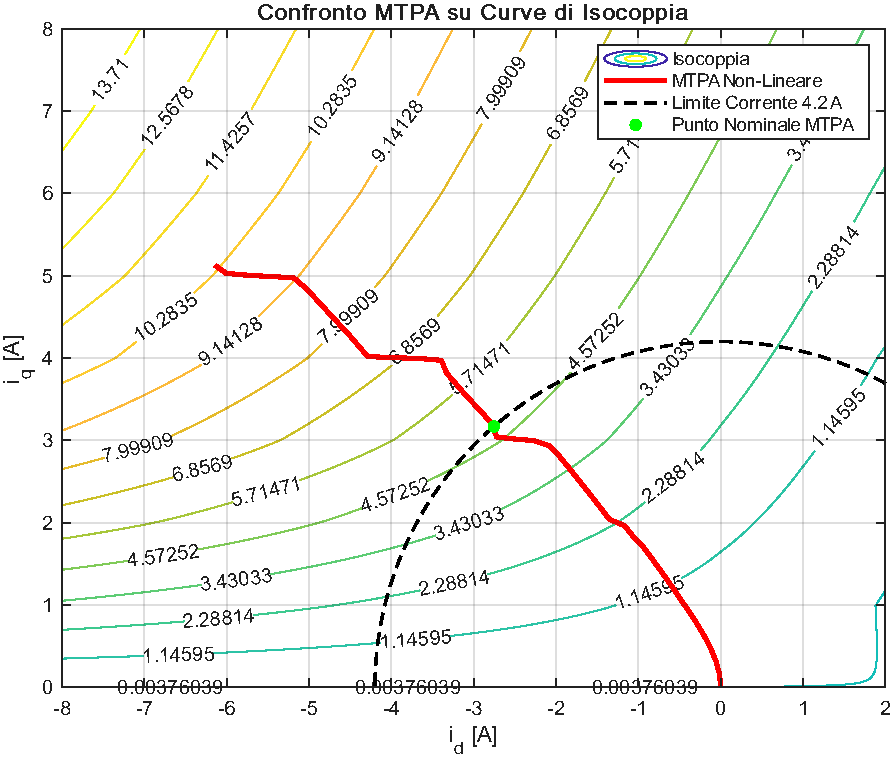
\includegraphics[height=8 cm]{immagini/MTPA/Risultati_MTPA.pdf}
    \caption{Curva MTPA del motore IPM. Il vincolo sulla corrente è rappresentato dall'arco di circonferenza.}
    \label{fig:Risultati_MTPA}
\end{figure}






\subsection{Analisi dell'andamento di $\lambda_{dq}$ al variare della corrente rispetto ai punti della curva MTPA}
Si procede quindi esaminando i grafici del flusso ottenuti muovendosi lungo la curva MTPA, utilizzando $\theta_m$ come parametro. Ciò significa che i flussi $\lambda_d$ e $\lambda_q$ sono stati calcolati rispetto ai punti di corrente lungo la curva.\\
Si può quindi analizzare varia il flusso $\lambda_d$ spostandosi lungo la curva MTPA (Figure \ref{fig:Flusso_D_vs_Id_MTPA_Specifictheta} e \ref{fig:Flusso_D_vs_Iq_MTPA_Specifictheta}).
Allo stesso modo si analizza come varia il valore di $\lambda_q$ spostandosi lungo la curva MTPA (Figure \ref{fig:Flusso_Q_vs_Id_MTPA_Specifictheta} e \ref{fig:Flusso_Q_vs_Iq_MTPA_Specifictheta}).\\
Si procede poi con l'analizzare l'andamento del flusso $\lambda_d$  rispetto alla corrente $i_d$ (Figura \ref{fig:MTPA_Flusso_D_vs_Iq_thetaVar}) e $i_q$ nominale (Figura \ref{fig:MTPA_Flusso_D_vs_Id_thetaVar}), mentre l'altra componente di corrente viene fatta variare.\\
In seguito, si effettua lo stesso tipo di analisi per il flusso $\lambda_q$ (Figura \ref{fig:MTPA_Flusso_Q_vs_Iq_thetaVar} e \ref{fig:MTPA_Flusso_Q_vs_Id_thetaVar}).\\
Il fatto che i grafici presentano delle variazioni nette di pendenza è dovuto all'andamento non lineare della curva MTPA.


\begin{figure}
\centering
    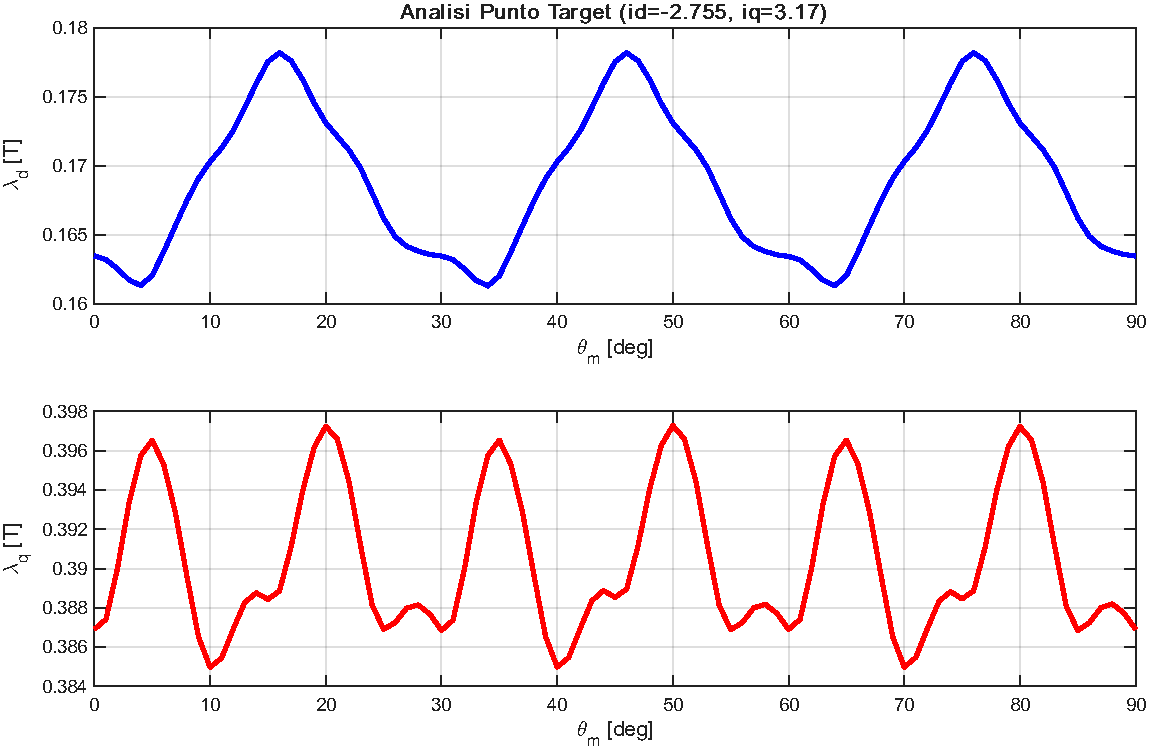
\includegraphics[height=8 cm]{immagini/MTPA/Confronto_Flussi_PuntoTarget_0.pdf}
    \caption{Andamento del flusso D e Q in corrispondenza del punto MTPA nominale a seconda della posizione meccanica $\theta_m$ @ $i_q$ = 3.224 A.}   
    \label{fig:Confronto_Flussi_PuntoTarget_0}
\end{figure}




\begin{figure}
\centering
    \includegraphics[height=8 cm]{immagini/MTPA/Flusso_D_vs_Id_MTPA_Specifictheta.pdf}
    \caption{Andamento di $\lambda_d$ in funzione di $i_d$ a seconda della posizione meccanica $\theta_m$, seguendo la curva MTPA.}    \label{fig:Flusso_D_vs_Id_MTPA_Specifictheta}
\end{figure}

\begin{figure}
\centering
    \includegraphics[height=8 cm]{immagini/MTPA/Flusso_D_vs_Iq_MTPA_Specifictheta.pdf}
    \caption{Andamento di $\lambda_d$ in funzione di $i_q$ a seconda della posizione meccanica $\theta_m$, seguendo la curva MTPA.}   \label{fig:Flusso_D_vs_Iq_MTPA_Specifictheta}
\end{figure}



\begin{figure}
\centering
    \includegraphics[height=8 cm]{immagini/MTPA/Flusso_Q_vs_Id_MTPA_Specifictheta.pdf}
    \caption{Andamento di $\lambda_q$ in funzione di $i_d$ a seconda della posizione meccanica $\theta_m$, seguendo la curva MTPA.}   \label{fig:Flusso_Q_vs_Id_MTPA_Specifictheta}
\end{figure}

\begin{figure}
\centering
    \includegraphics[height=8 cm]{immagini/MTPA/Flusso_Q_vs_Iq_MTPA_Specifictheta.pdf}
    \caption{Andamento di $\lambda_q$ in funzione di $i_q$ a seconda della posizione meccanica $\theta_m$, seguendo la curva MTPA.}   \label{fig:Flusso_Q_vs_Iq_MTPA_Specifictheta}
\end{figure}



\begin{figure}
\centering
    
\includegraphics[height=8 cm]{immagini/MTPA/Flusso_D_vs_Iq_thetaVar.pdf}
    \caption{Andamento del flusso D in funzione di $i_q$ a seconda della posizione meccanica $\theta_m$ @ $i_d$ = -2.755 A.}   
    \label{fig:MTPA_Flusso_D_vs_Iq_thetaVar}
\end{figure}

\begin{figure}
\centering
    
\includegraphics[height=8 cm]{immagini/MTPA/Flusso_D_vs_Id_thetaVar.pdf}
    \caption{Andamento del flusso D in funzione di $i_d$ a seconda della posizione meccanica $\theta_m$ @ $i_q$ = 3.224 A.}   
    \label{fig:MTPA_Flusso_D_vs_Id_thetaVar}
\end{figure}



\begin{figure}
\centering
    
\includegraphics[height=8 cm]{immagini/MTPA/Flusso_Q_vs_Iq_thetaVar.pdf}
    \caption{Andamento del flusso Q in funzione di $i_q$ a seconda della posizione meccanica $\theta_m$ @ $i_d$ = -2.775.}   
    \label{fig:MTPA_Flusso_Q_vs_Iq_thetaVar}
\end{figure}


\begin{figure}
\centering
    
\includegraphics[height=8 cm]{immagini/MTPA/Flusso_Q_vs_Id_thetaVar.pdf}
    \caption{Andamento del flusso Q in funzione di $i_d$ a seconda della posizione meccanica $\theta_m$ @ $i_q$ = 3.17.}   
    \label{fig:MTPA_Flusso_Q_vs_Id_thetaVar}
\end{figure}

\subsection{Analisi dell'andamento di $\lambda_{dq}$ al variare della posizione meccanica rispetto ai punti della curva MTPA}
Si può analizzare l'andamento di $\lambda_d$ e $\lambda_q$ sui punti della curva MTPA (Figure \ref{fig:Flusso_D_vs_theta_MTPA} e \ref{fig:Flusso_Q_vs_theta_MTPA}) al variare della posizione meccanica $\theta_m$. Si osserva anche come l'ampiezza delle oscillazioni aumenta all'aumentare della corrente in modulo.\\
In Figura \ref{fig:Flusso_Q_vs_theta_MTPA} si può osservare in dettaglio l'andamento di $\lambda_d$ e $\lambda_q$ in corrispondenza del punto nominale MTPA.
Successivamente si è valutato la dipendenza dalla posizione della differenza del flusso $\lambda_d$ lungo la curva MTPA e a corrente nulla, per ogni posizione meccanica (Figura \ref{fig:Differenza_Assoluta_Flusso_D_MTPA_Progression}):
\begin{equation}
   \lambda_d^A(i_{dq}) = \lambda_d({i_{dq}})\Big|_{{i_{dq}}\in \text{MTPA}}-\lambda_d(0,0)
\end{equation}
In Figura \ref{fig:Differenza_Flusso_D_MTPA_vs_Zero} si può vedere in dettaglio l'andamento per il punto nominale MTPA.\\
Il flusso può anche essere espresso in maniera relativa, dividendo per il flusso $\lambda_d$ a corrente nulla (Figura \ref{fig:Differenza_Relativa_Flusso_D_MTPA_Progression}):
\begin{equation}
   \lambda_d^{A,rel}(i_{dq}) = \frac{\lambda_d({i_{dq}})\Big|_{{i_{dq}}\in \text{MTPA}}-\lambda_d(0,0)}{\lambda_d(0,0)}
\end{equation}
Si è valutata anche la dipendenza dalla posizione della differenza del flusso $\lambda_1$ nel punto MTPA nominale e a corrente nominale (Figura \ref{fig:Differenza_Assoluta_Flusso_Q_MTPA_Progression}):
\begin{equation}
    \lambda_q^B(i_{dq})=\lambda_q({i_{dq}})\Big|_{{i_{dq}}\in \text{MTPA}}-\lambda_q({i_{dq}})\Big|_{{i_{dq}}\in \text{MTPA,nom}}
\end{equation}
Un'altra valutazione
Si può analizzare inoltre l'incidenza percentuale del ripple di flusso rispetto al  valore medio. I punti di corrente di test appartengono alla curva MTPA.\\
Si analizza poi il profilo del flusso magnetico in funzione della posizione senza la componente media (Figure \ref{fig:Ripple_Relativo_Flusso_D_MTPA} e \ref{fig:Ripple_Relativo_Flusso_Q_MTPA}).\\ In questo modo è possibile esaminare meglio l'impatto della dipendenza della posizione angolare sull'ampiezza di oscillazione.
In Figura \ref{fig:Ripple_Relativo_Flusso_D_MTPA} si può notare come l'ampiezza di oscillazione di $\lambda_d$ relativa aumenti all'aumentare del modulo della corrente. al contrario, l'oscillazione relativa di $\lambda_q$ diminuisce all'aumentare del modulo di corrente (Figura \ref{fig:Ripple_Relativo_Flusso_Q_MTPA}).


\begin{figure}
\centering
    \includegraphics[height=8 cm]{immagini/MTPA/Flusso_D_vs_theta_MTPA.pdf}
    \caption{Andamento del flusso D in funzione della posizione a seconda del punto della curva MTPA analizzato.}
    \label{fig:Flusso_D_vs_theta_MTPA}
\end{figure}

\begin{figure}
\centering
    \includegraphics[height=8 cm]{immagini/MTPA/Flusso_Q_vs_theta_MTPA.pdf}
    \caption{Andamento del flusso Q in funzione della posizione a seconda del punto della curva MTPA analizzato.}
    \label{fig:Flusso_Q_vs_theta_MTPA}
\end{figure}


\begin{figure}
\centering
    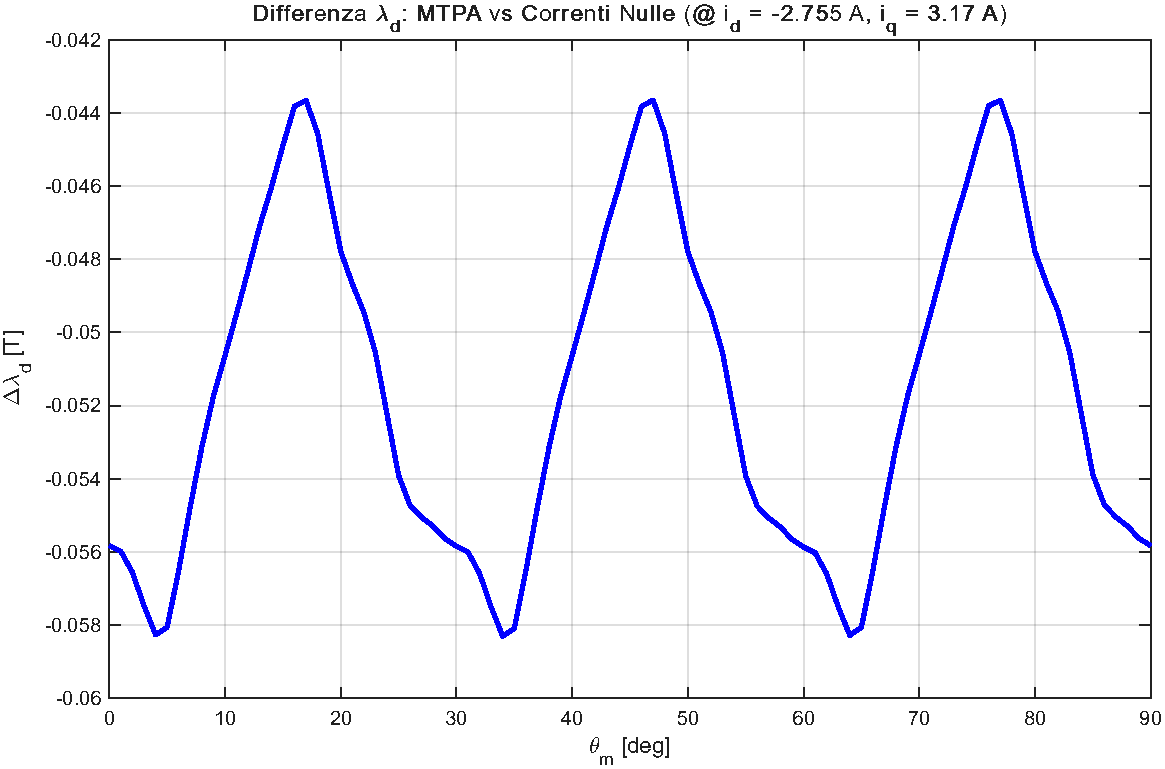
\includegraphics[height=8 cm]{immagini/MTPA/Differenza_Flusso_D_MTPA_vs_Zero.pdf}
    \caption{Differenza del flusso  nel punto MTPA nominale e a corrente nulla, per ogni posizione meccanica, in funzione di $\theta_M$ @ $i_d$ = -2.755, $i_q$ = 3.17 A.} 
    \label{fig:Differenza_Flusso_D_MTPA_vs_Zero}
\end{figure}



\begin{figure}
\centering
    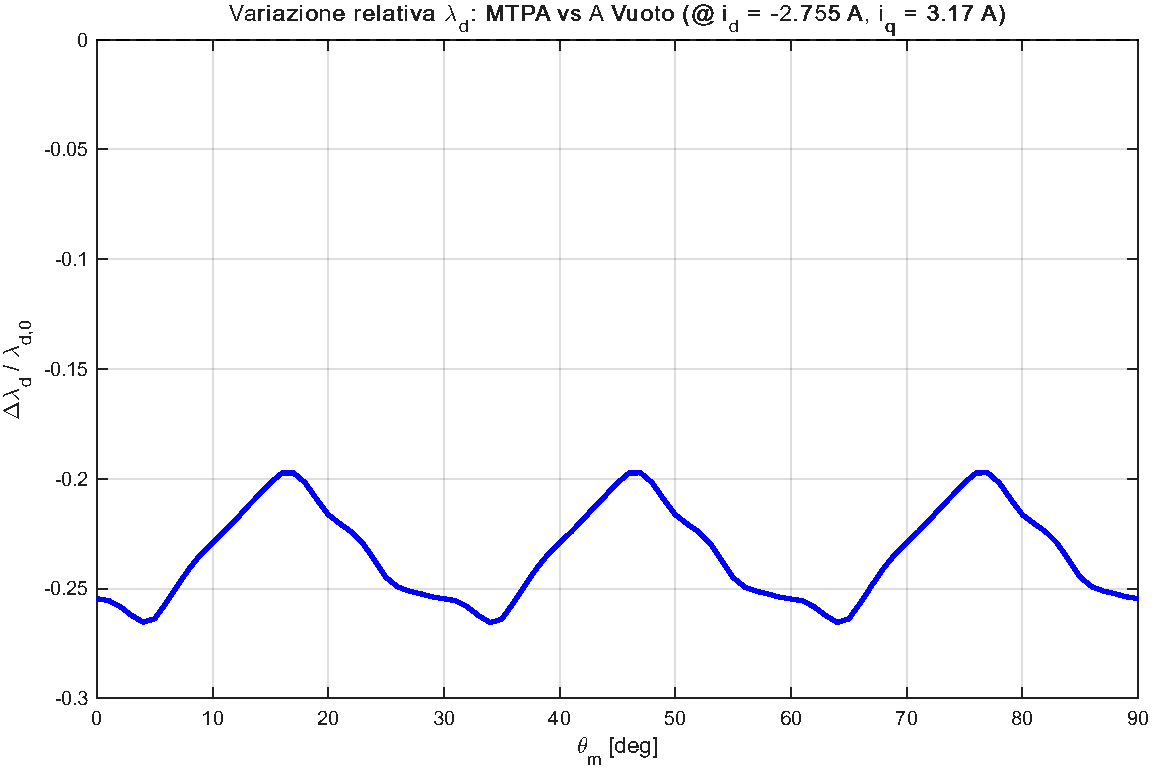
\includegraphics[height=8 cm]{immagini/MTPA/Differenza_Relativa_Flusso_D.pdf}
    \caption{Differenza del flusso  nel punto MTPA nominale e a corrente nulla, normalizzato sul flusso a corrente nulla, in funzione di $\theta_M$, nor @ $i_d$ = -2.755 A, $i_q$ = 3.17 A.} 
    \label{fig:Differenza_Relativa_Flusso_D}
\end{figure}



\begin{figure}
\centering
    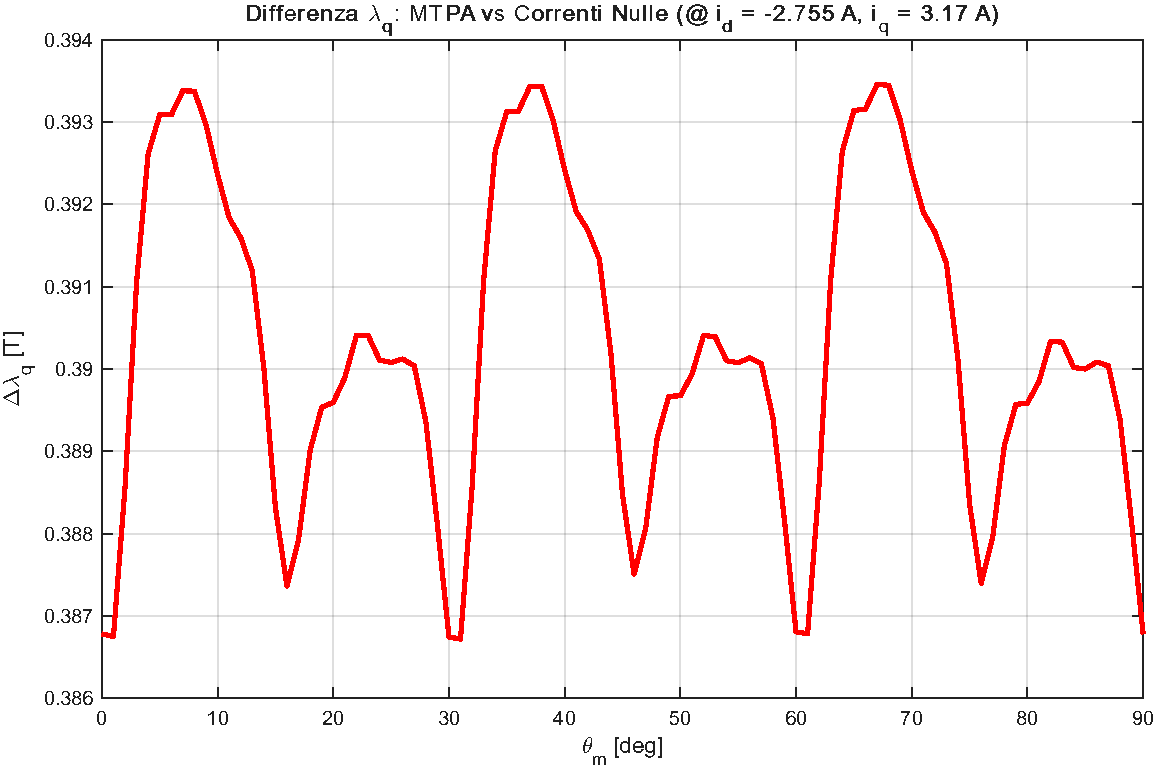
\includegraphics[height=8 cm]{immagini/MTPA/Differenza_Flusso_Q_MTPA_vs_Zero.pdf}
    \caption{Differenza del flusso Q in funzione di $\theta_M$, sottraendo il flusso Q a corrente nulla, @ $i_d$ = -2.755, $i_q$ = 3.17 A.} 
    \label{fig:Differenza_Flusso_Q_MTPA_vs_Zero}
\end{figure}

\begin{figure}
\centering
    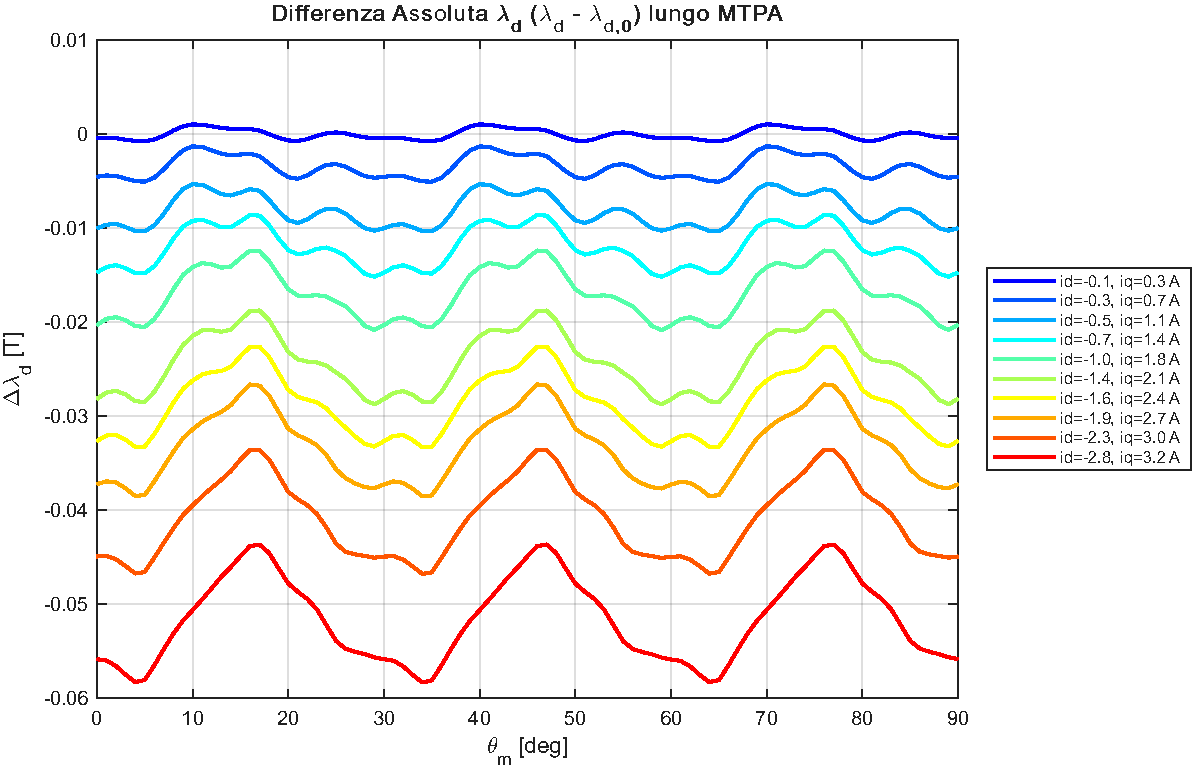
\includegraphics[height=8 cm]{immagini/MTPA/MTPA_multiplo/Differenza_Assoluta_Flusso_D_MTPA_Progression.pdf}
    \caption{Differenza del flusso Q in funzione di $\theta_M$, sottraendo il flusso D a corrente nulla, lungo la curva MTPA.} 
    \label{fig:Differenza_Assoluta_Flusso_D_MTPA_Progression}
\end{figure}

\begin{figure}
\centering
    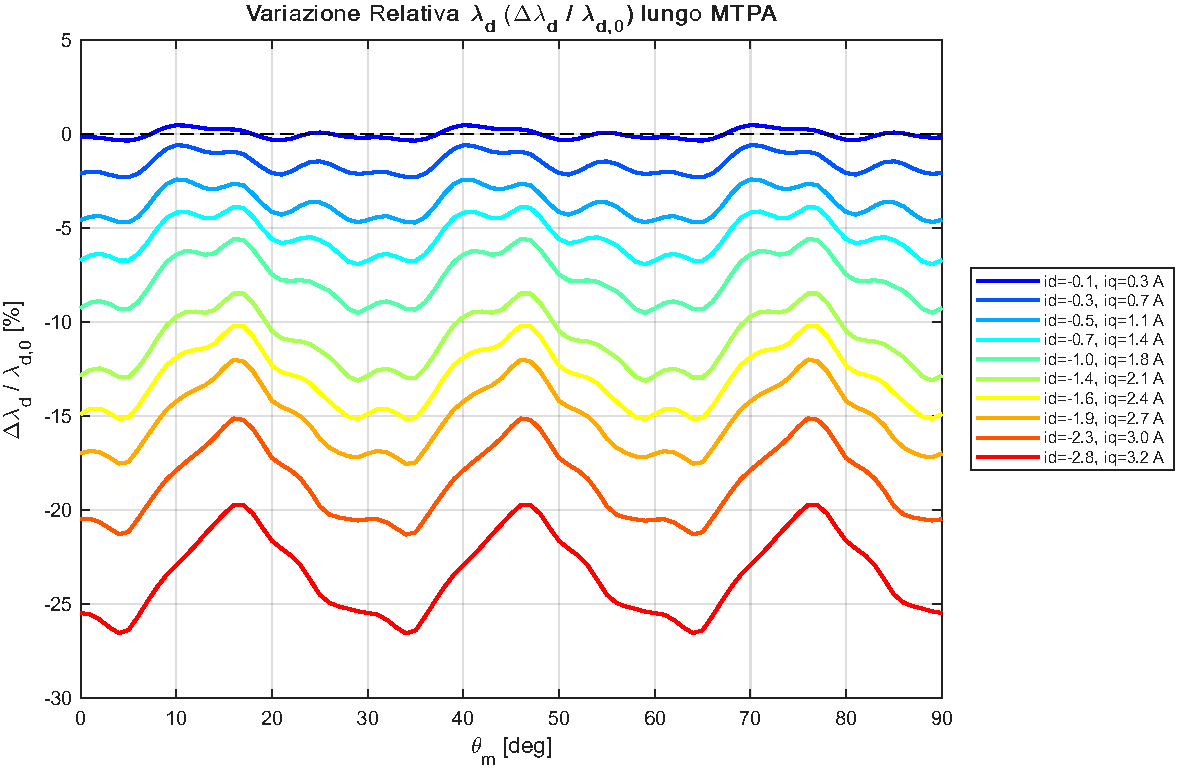
\includegraphics[height=8 cm]{immagini/MTPA/MTPA_multiplo/Differenza_Relativa_Flusso_D_MTPA_Progression.pdf}
    \caption{Differenza del flusso Q in funzione di $\theta_M$, sottraendo il flusso D a corrente nulla e dividendo per esso, lungo la curva MTPA.} 
    \label{fig:Differenza_Relativa_Flusso_D_MTPA_Progression}
\end{figure}


\begin{figure}
\centering
    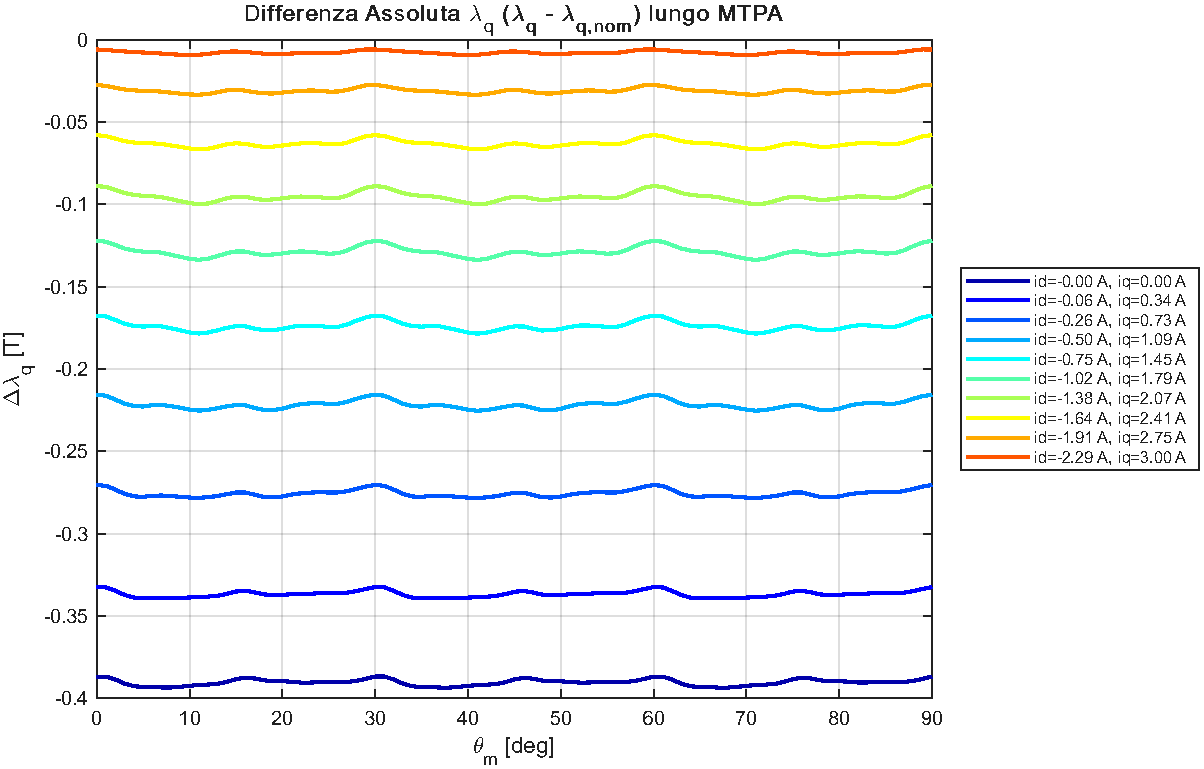
\includegraphics[height=8 cm]{immagini/MTPA/MTPA_multiplo/Differenza_Assoluta_Flusso_Q_MTPA_Progression.pdf}
    \caption{Differenza del flusso Q in funzione di $\theta_M$, sottraendo il flusso D a corrente nominale, lungo la curva MTPA.} 
    \label{fig:Differenza_Assoluta_Flusso_Q_MTPA_Progression}
\end{figure}

\begin{figure}
\centering
    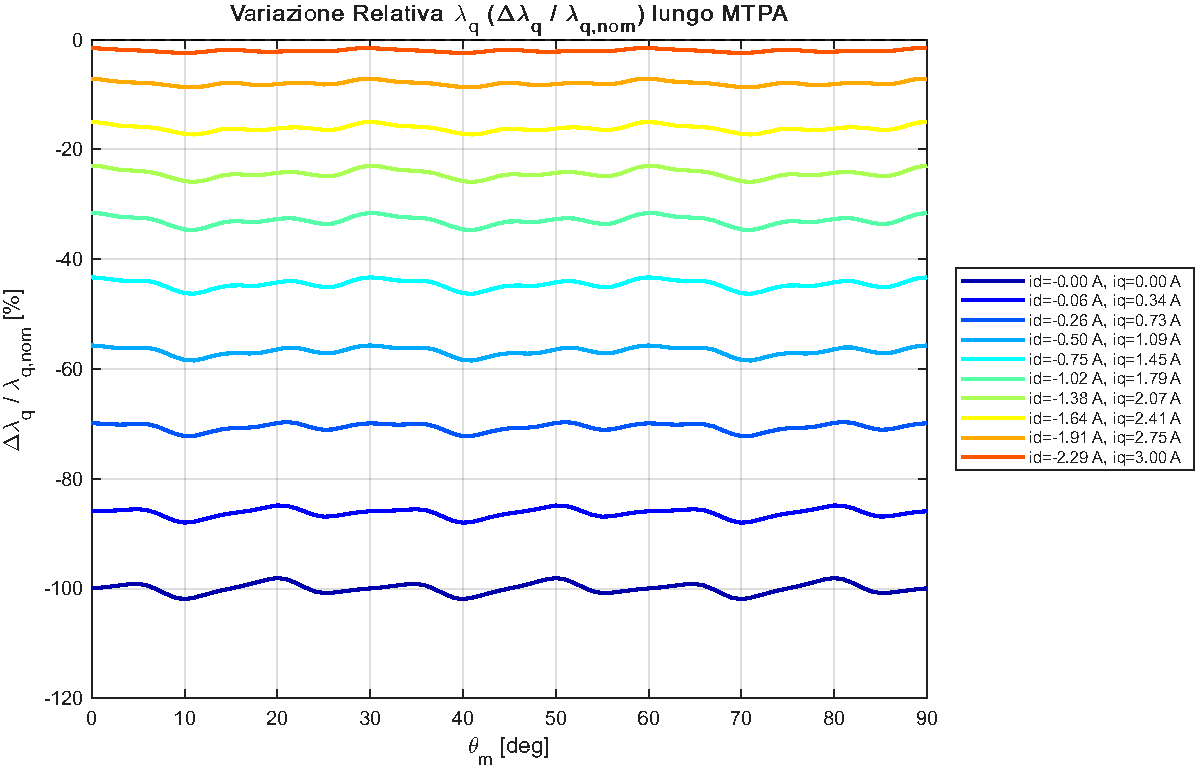
\includegraphics[height=8 cm]{immagini/MTPA/MTPA_multiplo/Differenza_Relativa_Flusso_Q_MTPA_Progression.pdf}
    \caption{Differenza del flusso Q in funzione di $\theta_M$, sottraendo il flusso D a corrente nominale e dividendo per esso, lungo la curva MTPA.} 
    \label{fig:Differenza_Relativa_Flusso_Q_MTPA_Progression}
\end{figure}



\begin{figure}
\centering
    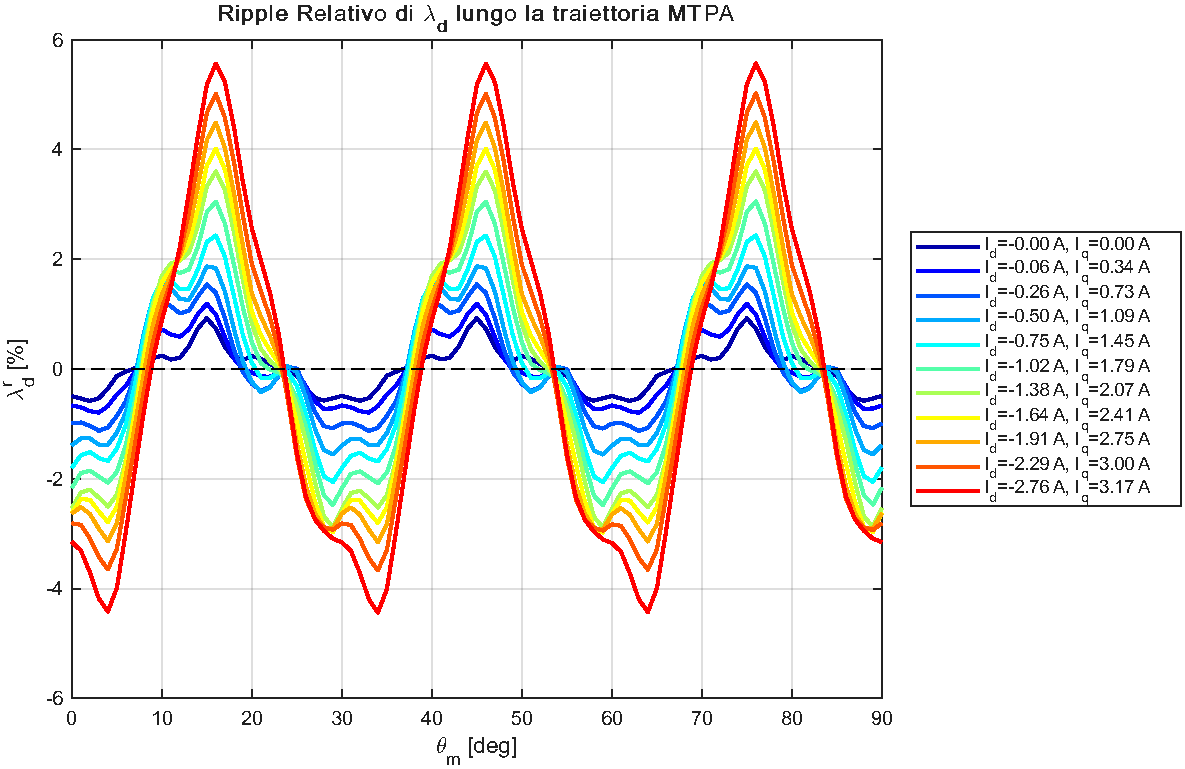
\includegraphics[height=8 cm]{immagini/MTPA/MTPA_multiplo/Ripple_Relativo_Flusso_D_MTPA.pdf}
    \caption{Variazione relativa del flusso D rispetto alla media.} 
    \label{fig:Ripple_Relativo_Flusso_D_MTPA}
\end{figure}



\begin{figure}
\centering
    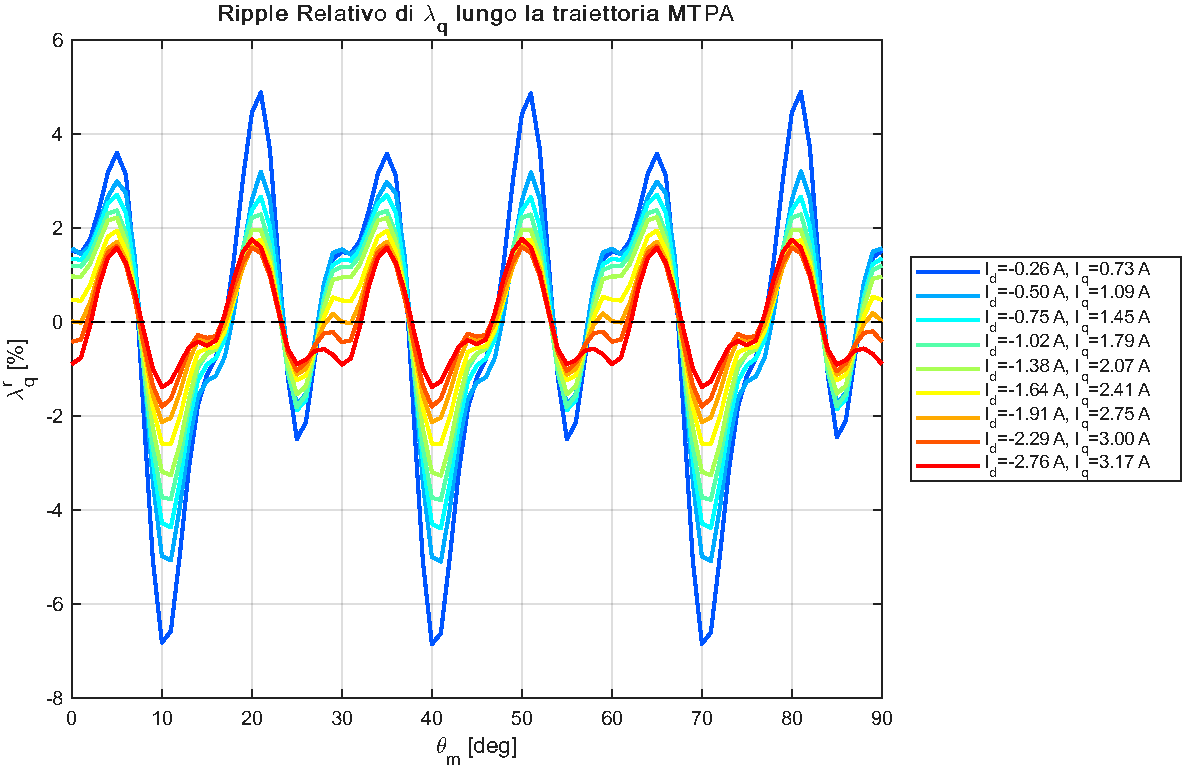
\includegraphics[height=8 cm]{immagini/MTPA/MTPA_multiplo/Ripple_Relativo_Flusso_Q_MTPA.pdf}
    \caption{Variazione relativa del flusso Q rispetto alla media.} 
    \label{fig:Ripple_Relativo_Flusso_Q_MTPA}
\end{figure}
\cleardoublepage
\chapter{Inversione delle mappe di flusso}
\label{chap:inversione}


 \section{Introduzione}
L'inversione delle mappe di flusso è un passaggio necessario per implementare il modello su Simulink.\\
Nelle mappe fornite del motore di Test, i flussi $\lambda_d$ e $\lambda_q$ sono espressi in funzione della corrente $i_d$, $i_q$ e della posizione meccanica $\theta_m$. Tramite l'inversione si esprimono le correnti $i_d$ e $i_q$ in 
funzione dei due flussi e della posizione meccanica.\\
Per invertire il flusso sono state adoperate due metodologie distinte:
\begin{enumerate}
\item Minimizzazione della funzione di costo.
\item Inversione della griglia attraverso dati sparsi: 

\end{enumerate}
\subsection{Minimizzazione della funzione di costo.}
La funzione di costo da minimizzare ha la seguente forma:
\begin{equation}
    J(\mathbf{i}_{dq}) = || \lambda_d^*(k) - \lambda_d(\mathbf{i}_{dq}, \theta_m) || + || \lambda_q^*(k) - \lambda_q(\mathbf{i}_{dq}, \theta_m) ||
\end{equation}
I vettori di flusso che costituiranno le nuove coordinate della mappa vengono generati usando la funzione \texttt{linspace}, creando un range di punti equispaziati tra i due limiti  imposti.\\
Tale funzione permette di trovare la coppia di correnti  $i_d$ e $i_q$ il cui flusso associato è quello più prossimo al flusso di target.\\
L'inversione del flusso magnetico viene eseguita per ogni posizione meccanica $\theta_m$. L'inversione produce quindi due matrici bidimensionali che esprimono le correnti $i_d$ e $i_q$ in funzione dei flussi $\lambda_d$ e $\lambda_q$. Per ottenere le mappe invertite complete tridimensionali, vengono concatenate le matrici bidimensionali ottenute per ogni posizione meccanica $\theta_m$.\\

\subsection{Inversione mediante dati sparsi}
Questo metodo è significativamente più rapido rispetto al precedente. La funzione di inversione riceve come input le mappe dirette di flusso $\lambda_d$ e $\lambda_q$. All'interno della funzione vengono anche definiti i vettori di flusso della mappa inversa. Essi rappresenteranno le coordinate della griglia. Gli estremi di tali vettori costituiscono gli estremi del dominio di flusso della mappa inversa.\\ Come viene spiegato nel Paragrafo \ref{sec:limiti_dominio_flusso} la scelta degli estremi di tali vettori è fondamentale, poichè la scelta di un range troppo ampio, può comportare ad errori nel processo di interpolazione.\\ L'inversione avviene passando alla funzione  \texttt{scatteredInterpolant} la terna di valori costituita dai flussi $\lambda_d$ e $\lambda_q$ e dalla corrente $i_d$ o $i_q$. Vengono creati così due  interpolatori, uno per $i_d$ e uno per $i_q$. Si passano come argomento ai due interpolatori le griglie di flusso della mappa inversa, ottenendo così le corrispondenti mappe di corrente.\\
Anche in questo caso l'inversione avviene per ogni posizione meccanica e poi si concatenano le matrici bidimensionali per ottenere le matrici 3D.

\section{Scelta degli estremi del dominio del flusso}
\label{sec:limiti_dominio_flusso}
È fondamentale definire con cautela gli estremi del dominio dei flussi per la mappa inversa. Infatti, l'utilizzo di un intervallo troppo esteso comporterebbe la presenza di punti (coppie di flusso e posizione angolare) a cui non è associata alcuna coppia di correnti nella mappa diretta. Ciò accade perché tali valori eccedono il flusso massimo della mappa diretta, uscendo così dal dominio di interpolazione.\\
Per ovviare a questo problema il limite superiore del dominio del flusso è stato imposto come il \textit{minimo tra i valori massimi} di flusso per ogni posizione angolare. In questo modo si è certi che a ogni coppia di elemetnti individuati dai vettori di flusso venga  associata una coppia di correnti plausibile. Seguendo lo stesso criterio, il limite inferiore  è stato imposto come il \textit{massimo tra i valori minimi} di flussi per ogni posizione angolare:



\begin{equation}
\begin{cases}
    \lambda_{d,max}^\text{Dom}  = \min_{\theta_m} \left( \max(\lambda_{d}(\theta_m)) \right) \\[10pt]
    \lambda_{d,min}^\text{Dom} = \max_{\theta_m} \left( \min(\lambda_{d}(\theta_m)) \right)
\end{cases}
\end{equation}

e analogamente per $\lambda_q$:

\begin{equation}
\begin{cases}
    \lambda_{q,max}^\text{Dom}  = \min_{\theta_m} \left( \max(\lambda_{q}(\theta_m)) \right) \\[10pt]
    \lambda_{q,min}^\text{Dom}  = \max_{\theta_m} \left( \min(\lambda_{q}(\theta_m)) \right)
\end{cases}
\end{equation}

Nel caso del motore di test, i range $\lambda_d$ e $\lambda_q$ presentano i seguenti valori estremi:
\begin{equation}
\begin{cases}
    \lambda_{d,min}^\text{Dom}  =  0.0567\ T \\[10pt]
    \lambda_{d,max}^\text{Dom}  =  0.2066\ T
\end{cases}
\qquad \text{e} \qquad
\begin{cases}
    \lambda_{q,min}^\text{Dom}  =  -0.5561\ T \\[10pt]
    \lambda_{q,max}^\text{Dom}  =  0.5559\ T
\end{cases}
\end{equation}
\begin{comment}
\subsection{Modello alternativo del motore}
Per evitare d'invertire le mappe di flusso, si possono utilizzare le induttanze differenziali.\\
Si possono ottenere calcolando il gradiente di $\lambda_d$ e $\lambda_q$ rispetto alle tre dimensioni: $i_d$,$i_q$ e $\theta_m$. 
\end{comment}

\section{Considerazioni sull'accuratezza della mappa invertita}
\label{sec:accuratezza_mappa}
Per verificare l'accuratezza della mappa ottenuta tramite inversione si può seguire la seguente procedura:

    \begin{enumerate}
    \item \textbf{Generazione dei vettori di test}: vengono definiti due vettori contenenti valori di test per i flussi $\lambda_d$ e $\lambda_q$. Per generare tali vettori, sono state usate le funzioni \texttt{logspace} e \texttt{linspace}, assicurandosi che tutti i punti di test non coincidano esattamente con i nodi della griglia originale.
    \item \textbf{Calcolo delle correnti corrispondenti}: attraverso le mappe invertite e l'algoritmo di interpolazione lineare (\texttt{interpn}), si determinano i valori di corrente $i_d$ e $i_q$ associati a ciascuna coppia di flussi di test.
    \item \textbf{Ritorno al valore di flusso}:  tramite le mappe dirette e la funzione "\texttt{interpn}" si calcolano i valori di flusso rispetto alla mappa iniziale.
    \item \textbf{Confronto tra i flussi ottenuti}: infine si calcola l'errore sottraendo ai flussi del vettore di test i flussi trovati nel passo precedente. L'errore può così essere analizzato con l'ausilio di un grafico.
    \end{enumerate}



\section{Analisi dei risultati}
Inizialmente si è utilizzata una mappa diretta con valori solo positivi di corrente $i_d$.\\ 
La mappa diretta di input alla funzione di inversione presenta il seguente range di corrente: $i_d \in [-10,\ 0] \ A$ e $i_q \in [-10,\ 10] \ A$.\\
Dall'analisi dei risultati ottenuti tramite il confronto dei flussi (l'errore è stato calcolato nel modo descritto nel Paragrafo  \ref{sec:accuratezza_mappa}), si nota la presenza di un errore consistente (Figure \ref{fig:errore_relativo_mappe_flusso_D_xcorrenti_DEPT} e \ref{fig:errore_relativo_mappe_flusso_Q_xcorrenti_DEPT}).\\
Al fine di ridurre l'errore si sono provate diverse soluzioni:
\begin{itemize}
    \item Infittimento della griglia di corrente
    \item Infittimento della griglia e estensione dei vincoli di flusso
    \item Estensione del dominio di corrente della mappa diretta di flusso con infittimento della griglia
\end{itemize}
I flussi sono stati confrontati rispetto alla stessa posizione angolare, $\theta_m$ = 49°.\\ La scelta dell'angolo è puramente esemplificativo, dato che il confronto rispetto ad altre posizioni angolari porta a risultati simili in termini di accuratezza.


\begin{figure}
\centering
    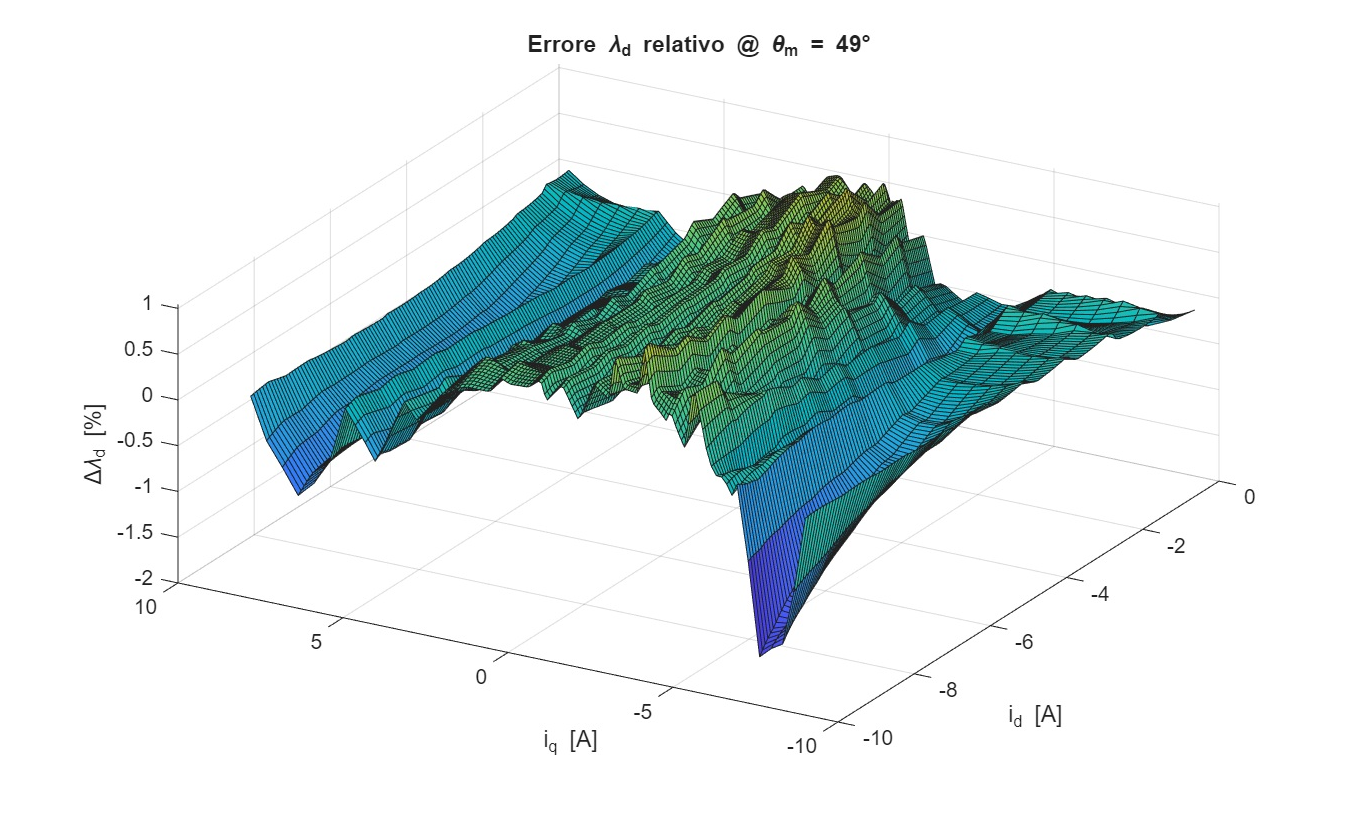
\includegraphics[height=8 cm]{immagini/errori_mappa_flusso/relativo/errore_relativo_mappe_flusso_D_xcorrenti_DEPT.pdf}
    \caption{Mappa dell'errore relativo su $\lambda_d$ (primo tentativo).}
    \label{fig:errore_relativo_mappe_flusso_D_xcorrenti_DEPT}
\end{figure}


\begin{figure}
\centering
    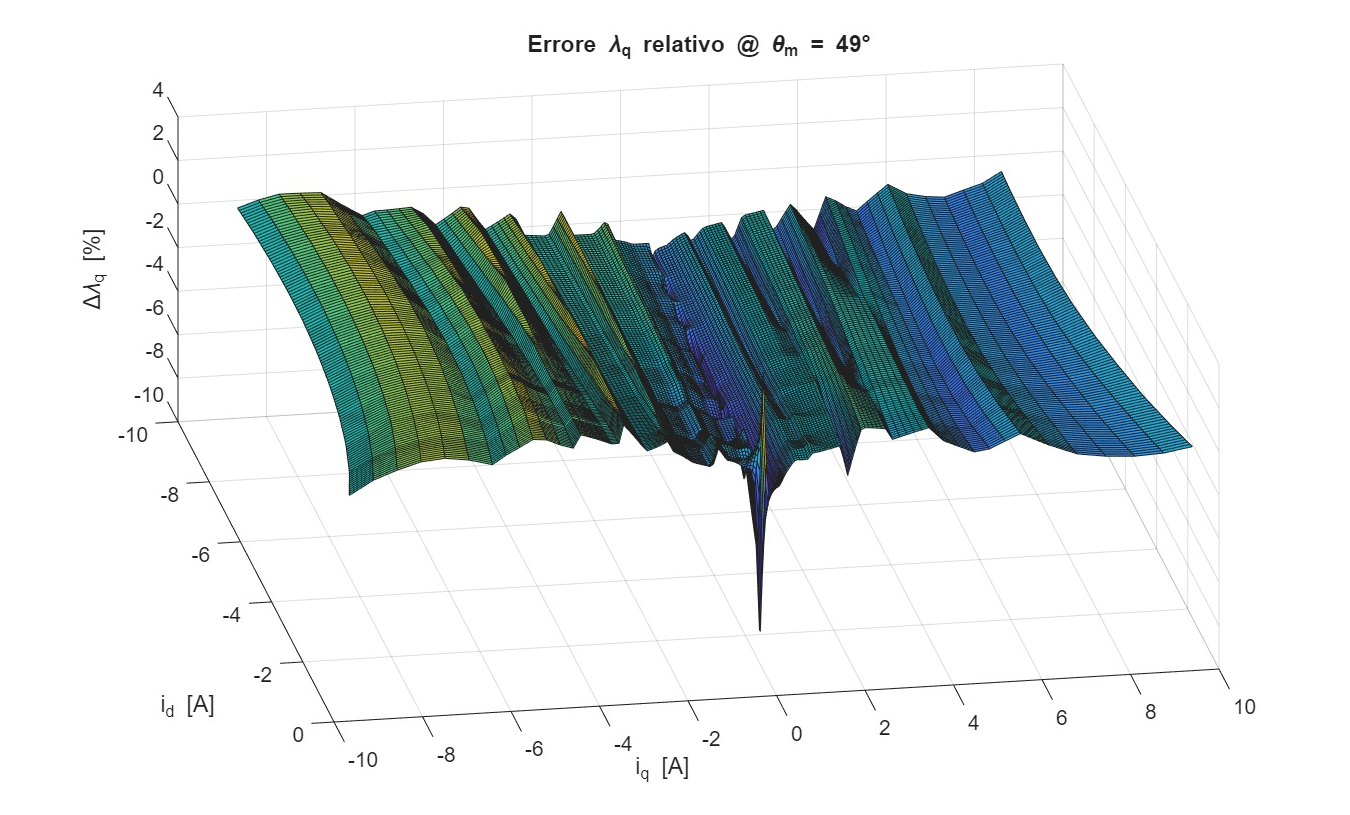
\includegraphics[height=8 cm]{immagini/errori_mappa_flusso/relativo/errore_relativo_mappe_flusso_Q_xcorrenti_DEPT.pdf}
    \caption{Mappa dell'errore relativo su $\lambda_q$ (primo tentativo).}
    \label{fig:errore_relativo_mappe_flusso_Q_xcorrenti_DEPT}
\end{figure}

\begin{figure}
\centering
    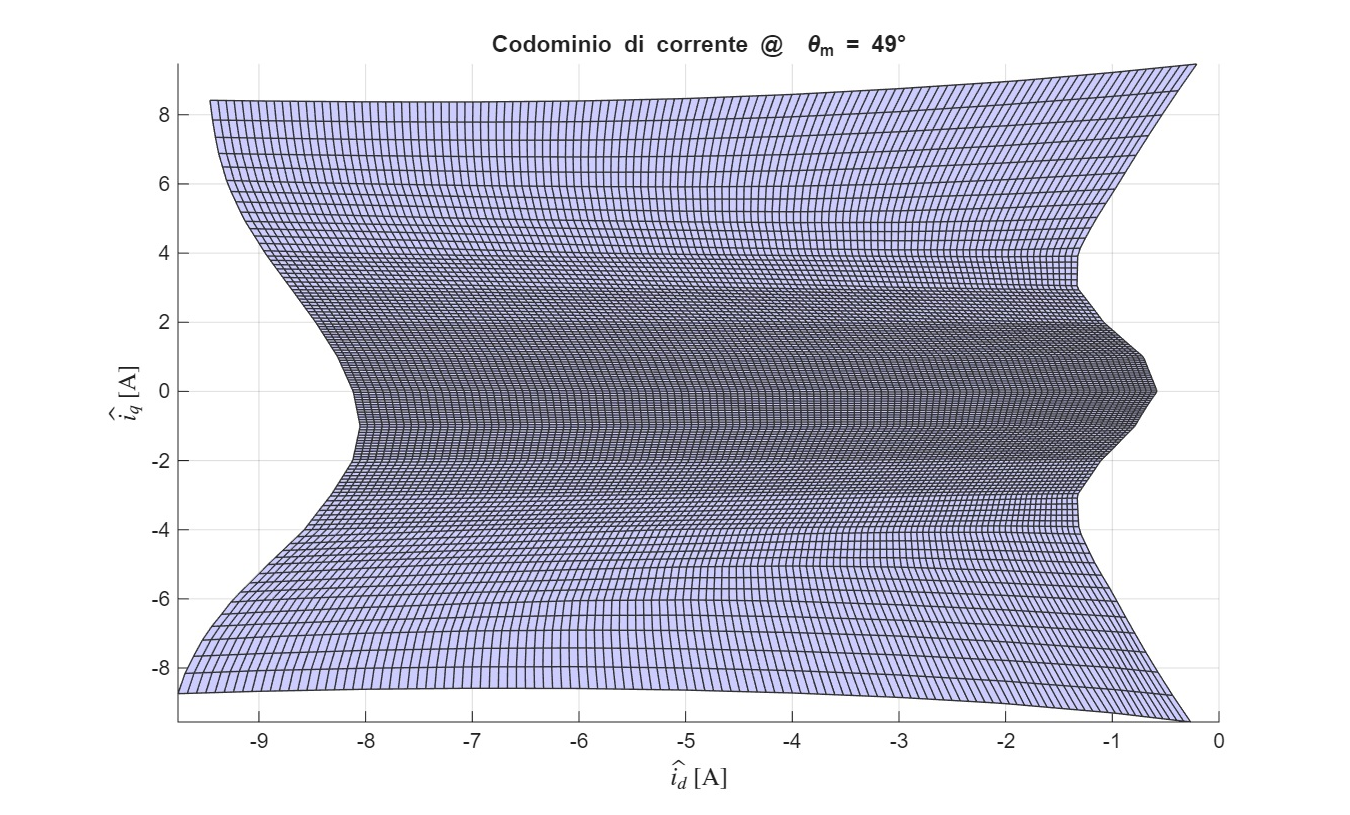
\includegraphics[height=8 cm]{immagini/errori_mappa_flusso/mappe_griglia/Mappa_correnti_UnicoColore_dense.pdf}
    \caption{Rappresentazione grafica del codominio di corrente (primo tentativo).}
    \label{fig:Mappa_lambdaD_UnicoColore_dense}
\end{figure}

\subsection{Infittimento della griglia di corrente}
Per diminuire tale errore si è infittita artificialmente la griglia di corrente delle mappe dirette di flusso, ovvero le mappe che vengono fornite alla funzione di inversione.
 In questo modo l'interpolatore \texttt{scatteredinterpolant} viene costruito a paritre da un maggior numero di punti. Si è osservato come ciò migliora considerevolmente l'accuratezza dell'inversione (Figure \ref{fig:errore_relativo_mappe_flusso_D_xcorrenti_dense} e \ref{fig:errore_relativo_mappe_flusso_Q_xcorrenti_dense}). 
Tuttavia, tale mappa inversa non comprende i valori di corrente prossimi a zero. Si veda a tal proposito la Figura \ref{fig:Mappa_lambdaD_UnicoColore_dense}. I nodi di tale grafico sono  tutti i punti di corrente associati alla griglia di flusso della mappa inversa. La griglia di flusso è costituita da tutte le combinazioni degli elementi dei vettori di flusso $\lambda_d$ e $\lambda_q$ che costituiscono le coordinate della mappa inversa.

\begin{figure}
\centering
    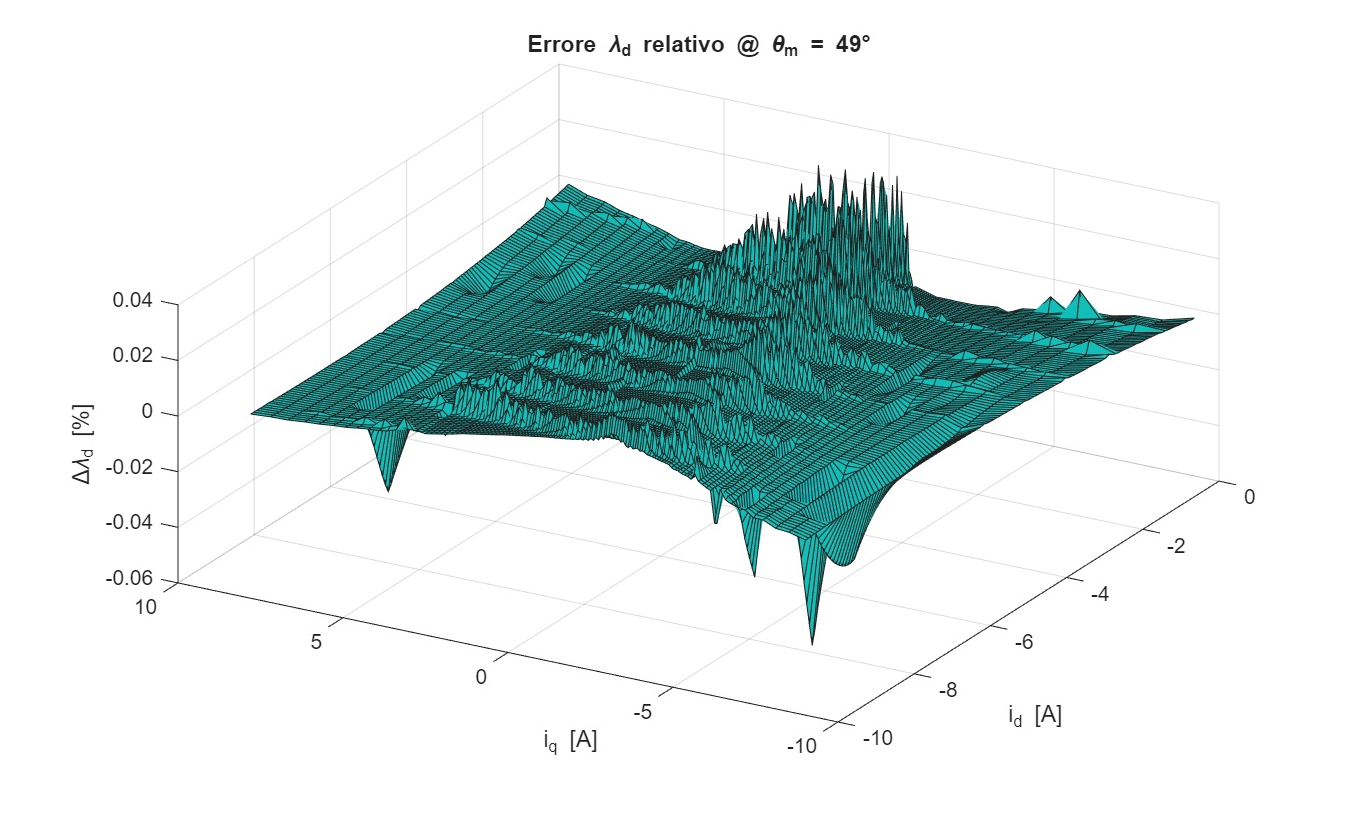
\includegraphics[height=8 cm]{immagini/errori_mappa_flusso/relativo/errore_relativo_mappe_flusso_D_xcorrenti_dense.pdf}
    \caption{Mappa dell'errore relativo su $\lambda_d$ con estensione dei vincoli di flusso.}
    \label{fig:errore_relativo_mappe_flusso_D_xcorrenti_dense}
\end{figure}


\begin{figure}
\centering
    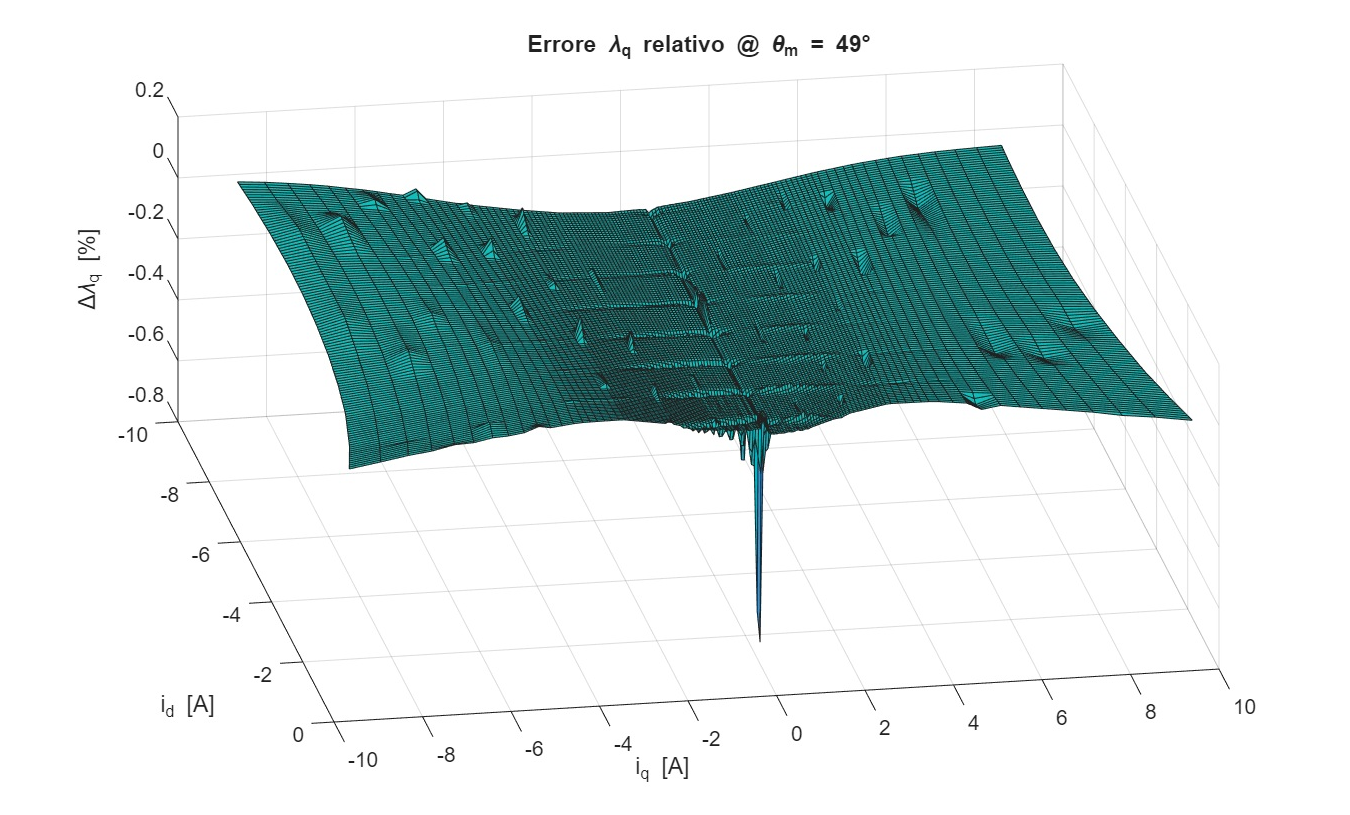
\includegraphics[height=8 cm]{immagini/errori_mappa_flusso/relativo/errore_relativo_mappe_flusso_Q_xcorrenti_dense.pdf}
    \caption{Mappa dell'errore relativo su $\lambda_q$ con infittimento della griglia.}
    \label{fig:errore_relativo_mappe_flusso_Q_xcorrenti_dense}
\end{figure}

\subsection{Infittimento della griglia e estensione dei vincoli di flusso}
Analizzando la stima del flusso per certi punti operativi, si è notata la presenza di un errore significativo di stima.\\
Questa inaccuratezza è stata ricondotta al fatto che l'estremo superiore del vettore  di flusso $\lambda_d$ risulta essere inferiore rispetto al flusso massimo associato a certi punti operativi. Ciò è vero, per esempio, per corrente nulla dove il flusso $\lambda_d$ è  massimo.\\
Pe aumentare l'accuratezza si è provato ad aumentare il range del dominio del flussi $\lambda_d$ e $\lambda_q$ della mappa invertita (Figure \ref{fig:errore_relativo_mappe_flusso_D_xcorrenti_ext} e \ref{fig:errore_relativo_mappe_flusso_Q_xcorrenti_ext}). 
Tuttavia, ciò comporta un aumento significativo dell'errore per correnti prossime a zero. La ragione di questo comportamento, come già discusso nel Paragrafo \ref{sec:limiti_dominio_flusso}, è che si introducono dei punti spuri nella stima del flusso. A una coppia di elementi dei vettori di flusso potrebbe non essere associato nessun valore di corrente nella mappa diretta. L'interpolatore quindi associa a tali valori di flusso dei valori di corrente irrealistici. \\
Ciò conferma che è necessario agire sulla mappa diretta di input alla funzione di inversione.





\begin{figure}
\centering
    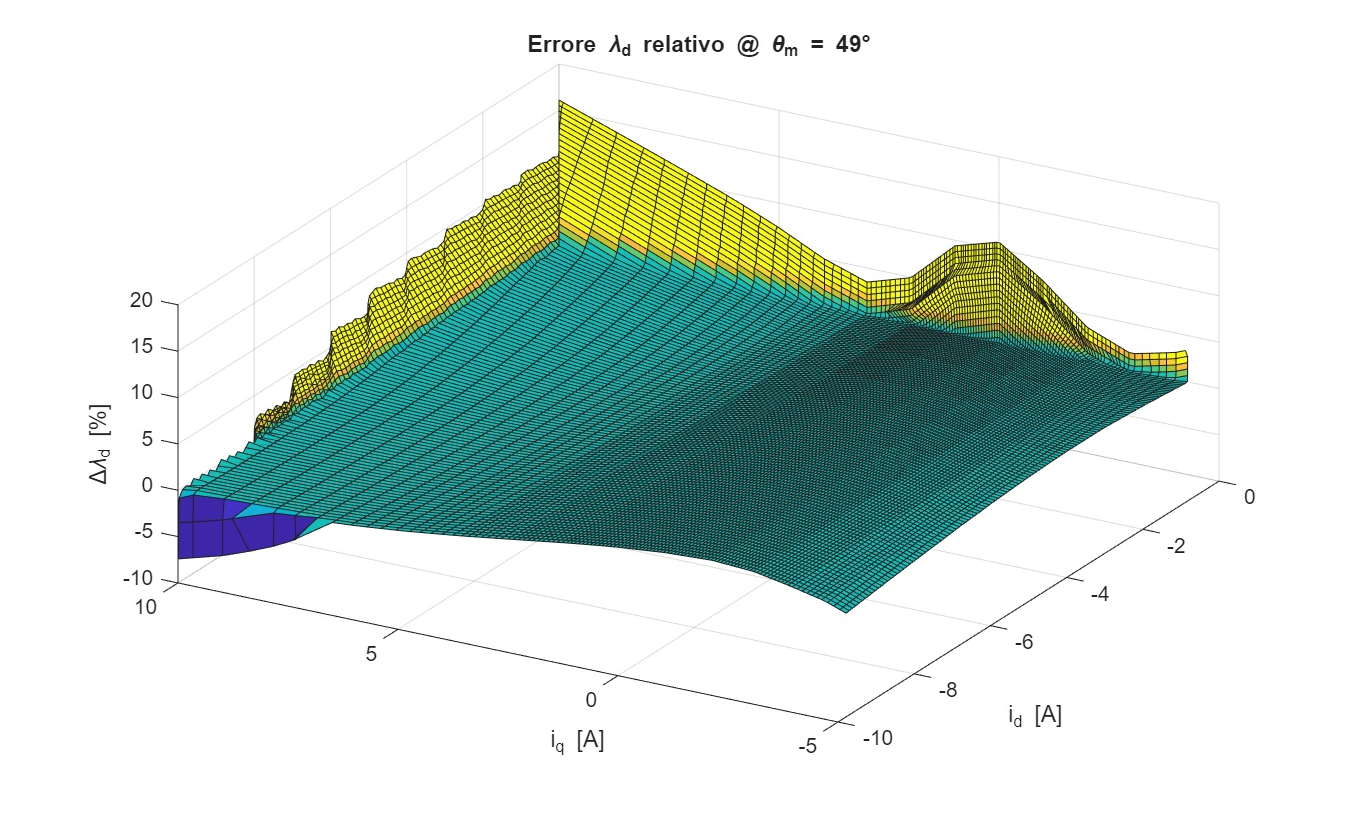
\includegraphics[height=8 cm]{immagini/errori_mappa_flusso/relativo/errore_relativo_mappe_flusso_D_xcorrenti_ext.pdf}
    \caption{Mappa dell'errore relativo su $\lambda_d$ con estensione dei vincoli di flusso.}
    \label{fig:errore_relativo_mappe_flusso_D_xcorrenti_ext}
\end{figure}


\begin{figure}
\centering
    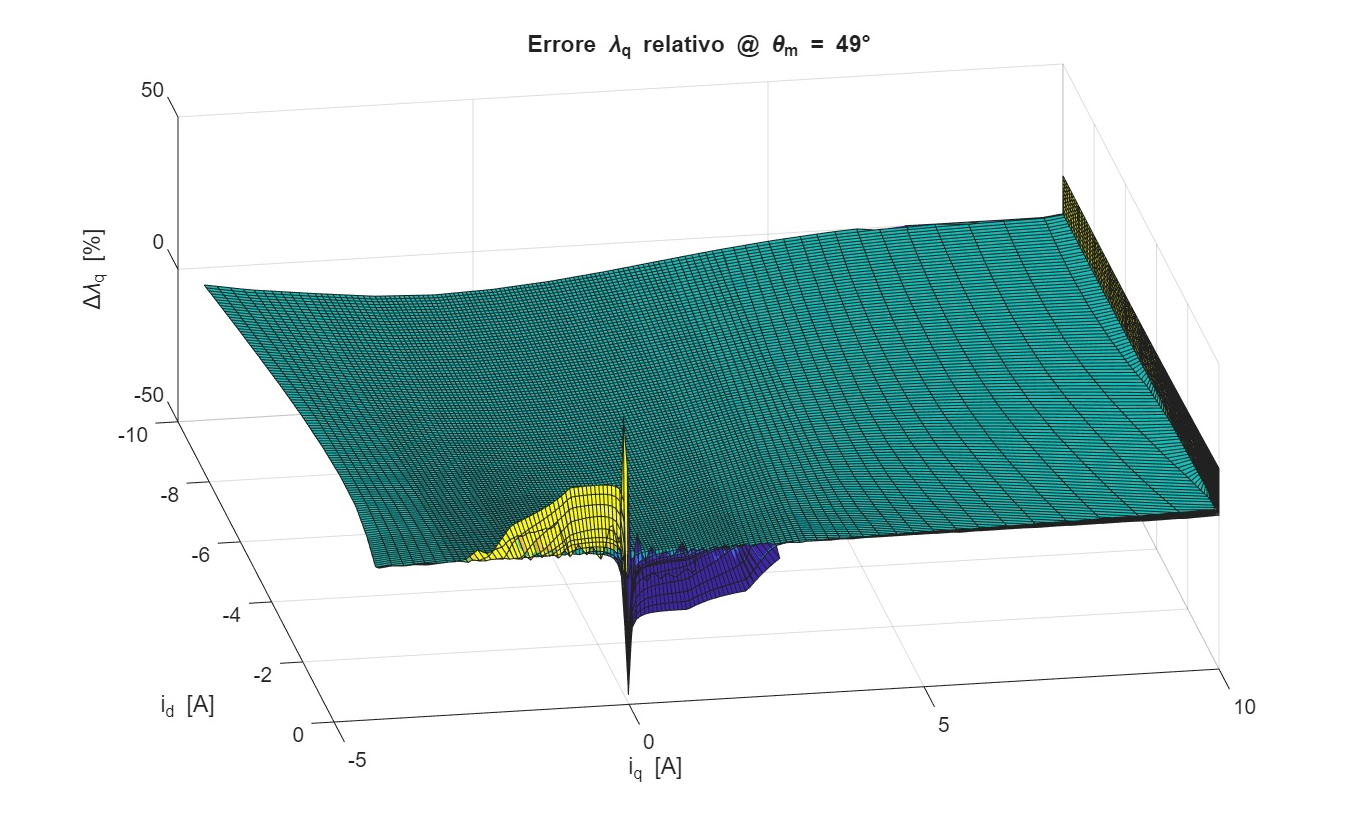
\includegraphics[height=8 cm]{immagini/errori_mappa_flusso/relativo/errore_relativo_mappe_flusso_Q_xcorrenti_ext.pdf}
    \caption{Mappa dell'errore relativo su $\lambda_q$ con estensione dei vincoli di flusso.}  \label{fig:errore_relativo_mappe_flusso_Q_xcorrenti_ext}
\end{figure}






\subsection{Estensione del dominio di corrente della mappa diretta di flusso con infittimento della griglia}
Per cercare di ridurre l'errore, si è espanso il dominio della mappa di corrente diretta iniziale anche per valori positivi di $i_d$ (Figure \ref{fig:errore_relativo_mappe_flusso_D_xcorrenti_positive} e \ref{fig:errore_relativo_mappe_flusso_Q_xcorrenti_positive}).\\ Il range della corrente della mappa diretta risulta così: 
$i_d \in [-8,\ 2] \ A$ e $i_q \in [-8,\ 8] \ A$.\\
In questo modo cambiano anche i vincoli della corrente, stabiliti utilizzando il procedimento del Paragrafo \ref{sec:limiti_dominio_flusso}. Tali vincoli risultano infatti pari a $0.0871 \ T$ e $0.2515 \ T$ per il flusso $\lambda_d$ e pari a $-0.5196 \ T$ e $0.5199 \ T$ per il flusso $\lambda_q$.
Si sono modificati anche i vincoli superiori di $i_d$ e $i_q$, dato che, essendo la corrente nominale pari a $4.2\ A$, avere un range troppo ampio risulta superfluo.\\
 Come si può notare in questo modo il codominio di corrente copre anche i valori intorno allo 0 (Figura \ref{fig:Mappa_lambdaD_UnicoColore_positive}). 



\begin{comment}

Si è provato ad estendere quindi il dominio del flusso oltre i limiti imposti in precedenza. Tuttavia, questa procedura comporta notevoli errori di stima vicino allo zero (Figura \ref{fig:errore_relativo_mappe_flusso_D_xcorrenti_ext}). 10pt
\end{comment}



\begin{comment}
\subsection{Valutazioni dei risultati ottenuti tramite la mapp inversa}
Nonostante la mappa inversa ottenuta dall'estensione della griglia di corrente iniziale risulti la più accurata, è ancora presente un errore di stima.\\
Per visualizzare tale errore, si è riportato a titolo esempleficativo un confronto tra il flusso reale e il flusso ottenuto implementando la mappa inversa per un dato punto operativo di corrente.
\end{comment}
\begin{figure}
\centering
    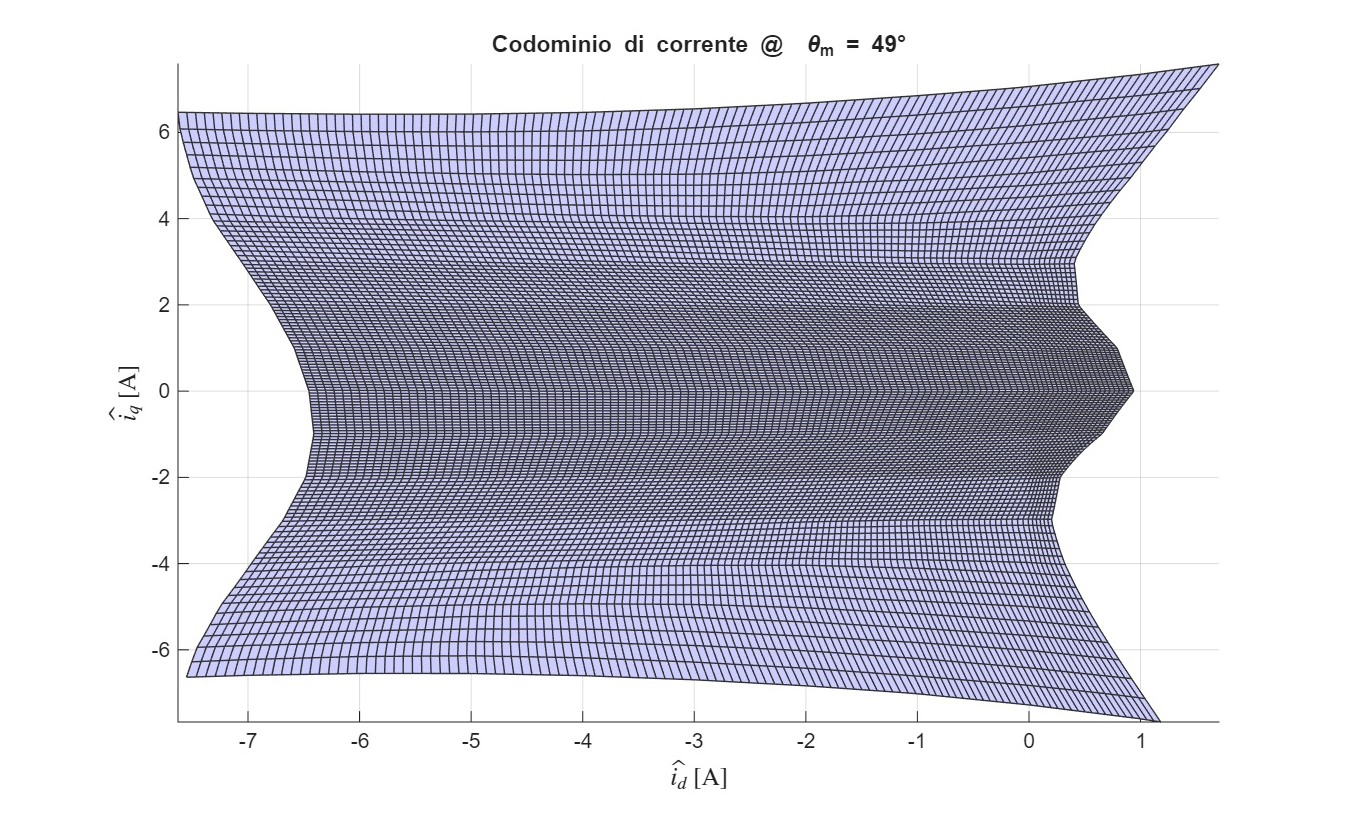
\includegraphics[height=8 cm]{immagini/errori_mappa_flusso/mappe_griglia/Mappa_correnti_UnicoColore_positive.pdf}u
    \caption{Rappresentazione grafica del codominio di corrente (quarto tentativo).}
    \label{fig:Mappa_lambdaD_UnicoColore_positive}
\end{figure}


\begin{figure}
\centering
    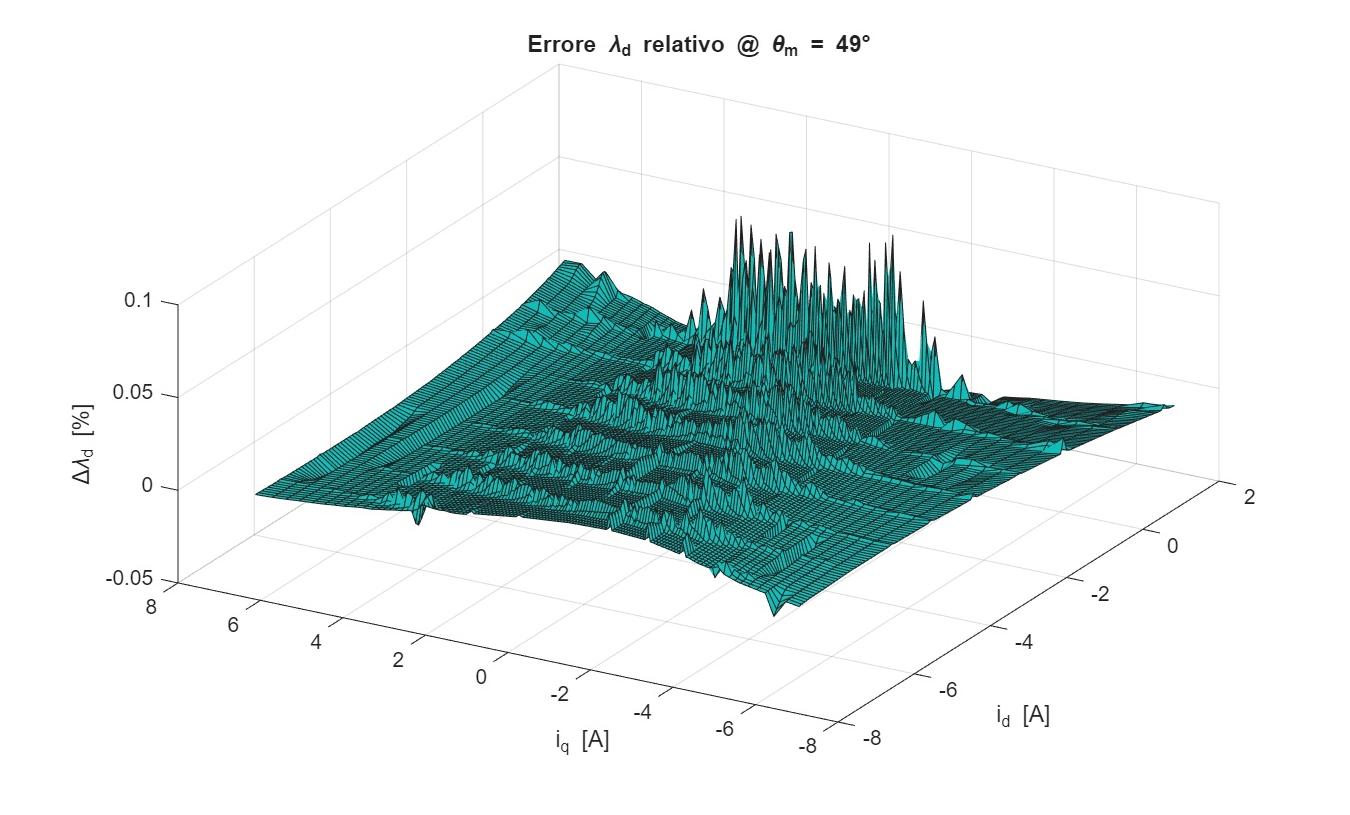
\includegraphics[height=8 cm]{immagini/errori_mappa_flusso/relativo/errore_relativo_mappe_flusso_D_xcorrenti_positive.pdf}
    \caption{Mappa dell'errore relativo su $\lambda_d$ con range positivo di corrente.}
    \label{fig:errore_relativo_mappe_flusso_D_xcorrenti_positive}
\end{figure}


\begin{figure}
\centering
    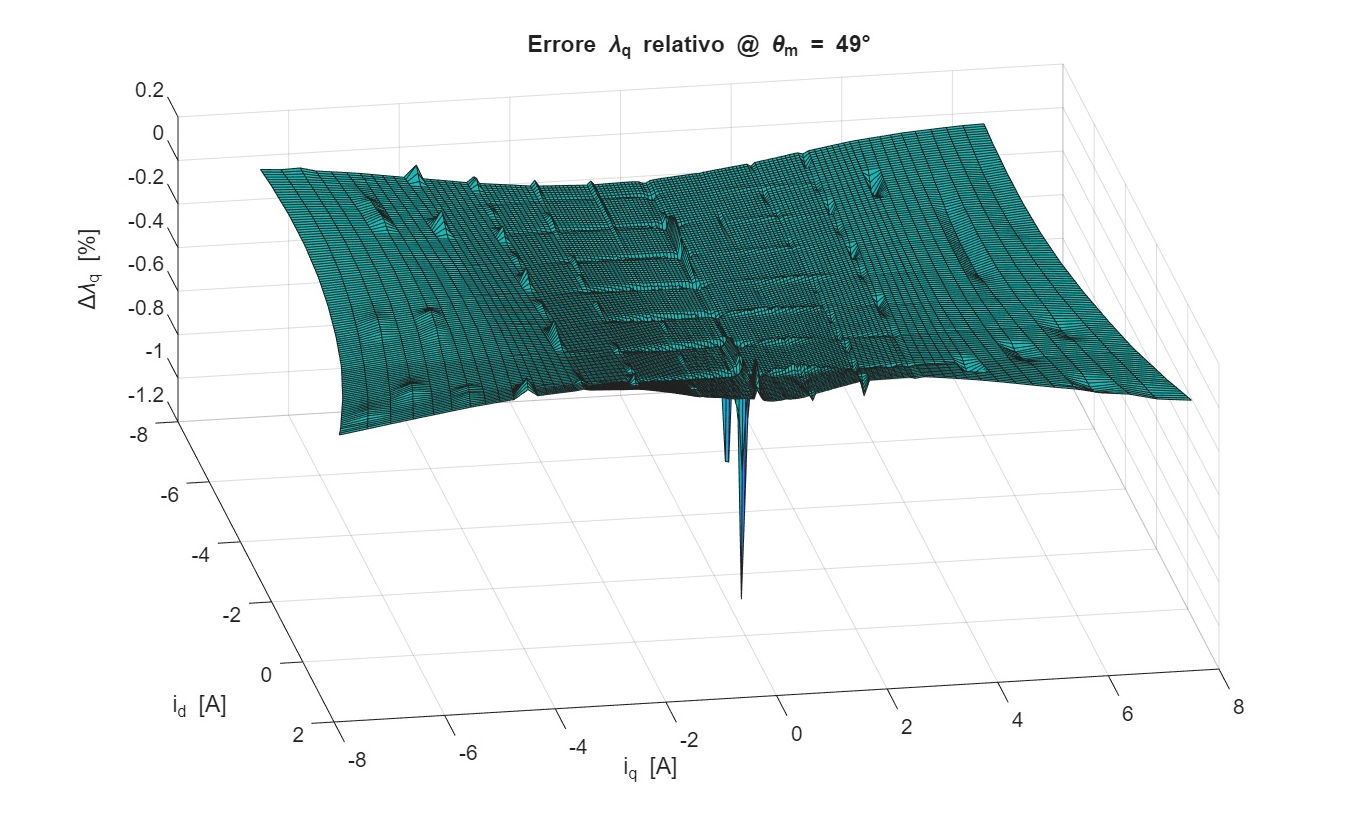
\includegraphics[height=8 cm]{immagini/errori_mappa_flusso/relativo/errore_relativo_mappe_flusso_Q_xcorrenti_positive.pdf}
    \caption{Mappa dell'errore relativo su $\lambda_q$ con range positivo di corrente.}  
    \label{fig:errore_relativo_mappe_flusso_Q_xcorrenti_positive}
\end{figure}


\cleardoublepage
\chapter{Creazione del modello Simulink}

\section{Creazione del modello Simulink}
Prima di validare il set-up sperimentale costituito, è necessario verificare il corretto funzionamento del sistema tramite un modello Simulink.\\
Si è innanzitutto implementato la procedura di misurazione. Per semplificare la sua costruzione, si è considerato la velocità del motore di test costante.\\
Si assume anche che le componenti di corrente d-q seguano perfettamente il riferimento.\\
In seguito verrà realizzato il modello completo, considerando anche il motore controllato in velocità che trascina il motore di test.\\

\section{Controllo di corrente}
Per controllare il motore si è utilizzato un controllo PID proporzionale integrale. Si è implementato anche un sistema Feedforward per eliminare il cross-coupling.\\
Tutti i blocchi per il controllo di corrente sono stati realizzati nel discreto.
È importante notare come questo sia possibile perché il valore di induttanza da utilizzare per il FFW è fornita dal datsaheet. In un caso reale, in cui tale valore non sia noto, non è possibile eseguire tale procedura.\\
 I parametri del controllore PID sono stati tarati manualmente per evitare sovraelongazioni e oscillazioni di corrente.\\
I controllori PID sono provvisti anche di anti-windup per evitare la saturazione dell'azione integrale.






\begin{figure}
\centering
    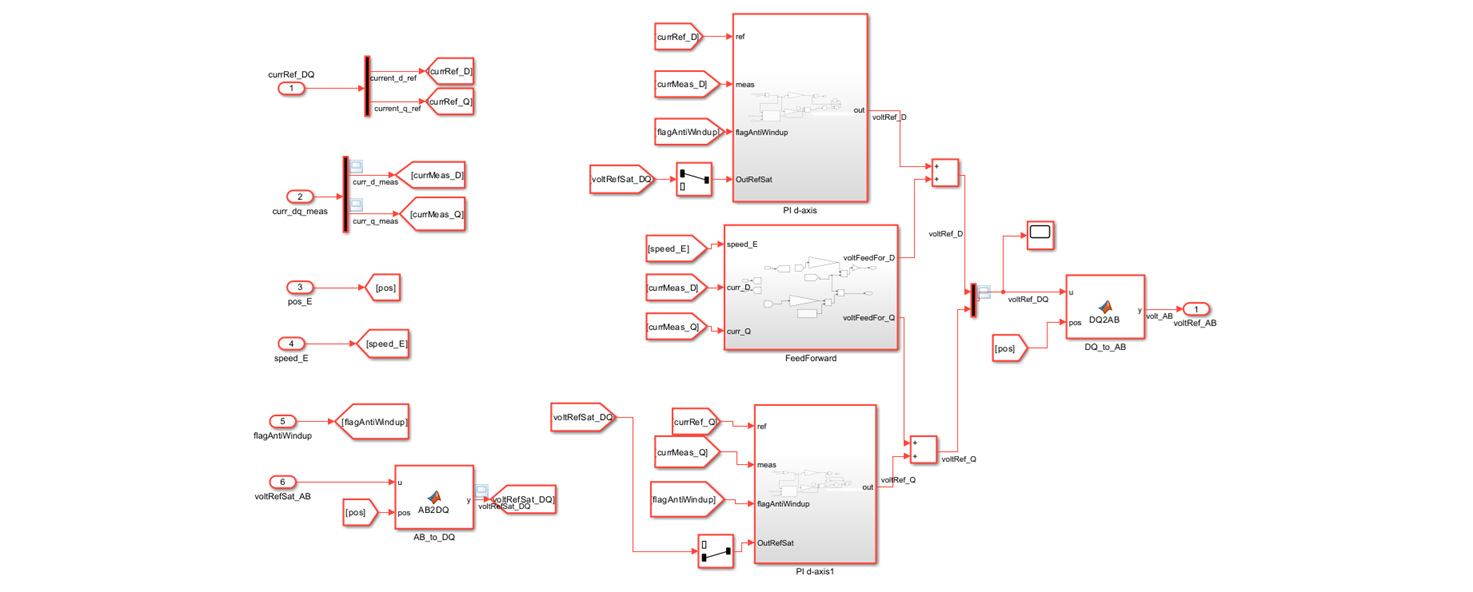
\includegraphics[height=8 cm]{immagini/immagini_motore/controllo_corrente_motore.png}
    \caption{Blocchi di controllo di corrente del motore.} 
    \label{fig:controllo_corrente_motore}
\end{figure}

\section{Implementazione della macchina a stati}

La procedura di misurazione può essere suddivisa in cin cinque fasi principali: 
\begin{enumerate}
    \item Fase di stima della resistenza di statore
    \item Fase di variazione di corrente
    \item Fase di attesa dello zero meccanico
    \item Fase di misurazione
    \item Conclusione della procedura
\end{enumerate}
Per gestire le varie fasi della procedura è stato utilizzato il blocco \texttt{Stateflow} di \texttt{SIMULINK}.\\
Per tenere traccia dello stato di avanzamento della procedura, il blocco \texttt{Stateflow} utilizza il contatore \texttt{stato}. Tale variabile è iizializzata a  0 e viene incrementata di 1 al termine di ogni fase di variazione di corrente e misurazione. Raggiunto il valore 6, il sistema di controllo porta le correnti a 0 e termina l'operazione.\\\
Uno schema della procedura è riportato in Figura \ref{fig:flowchart_stati}.

\begin{figure}
\centering
    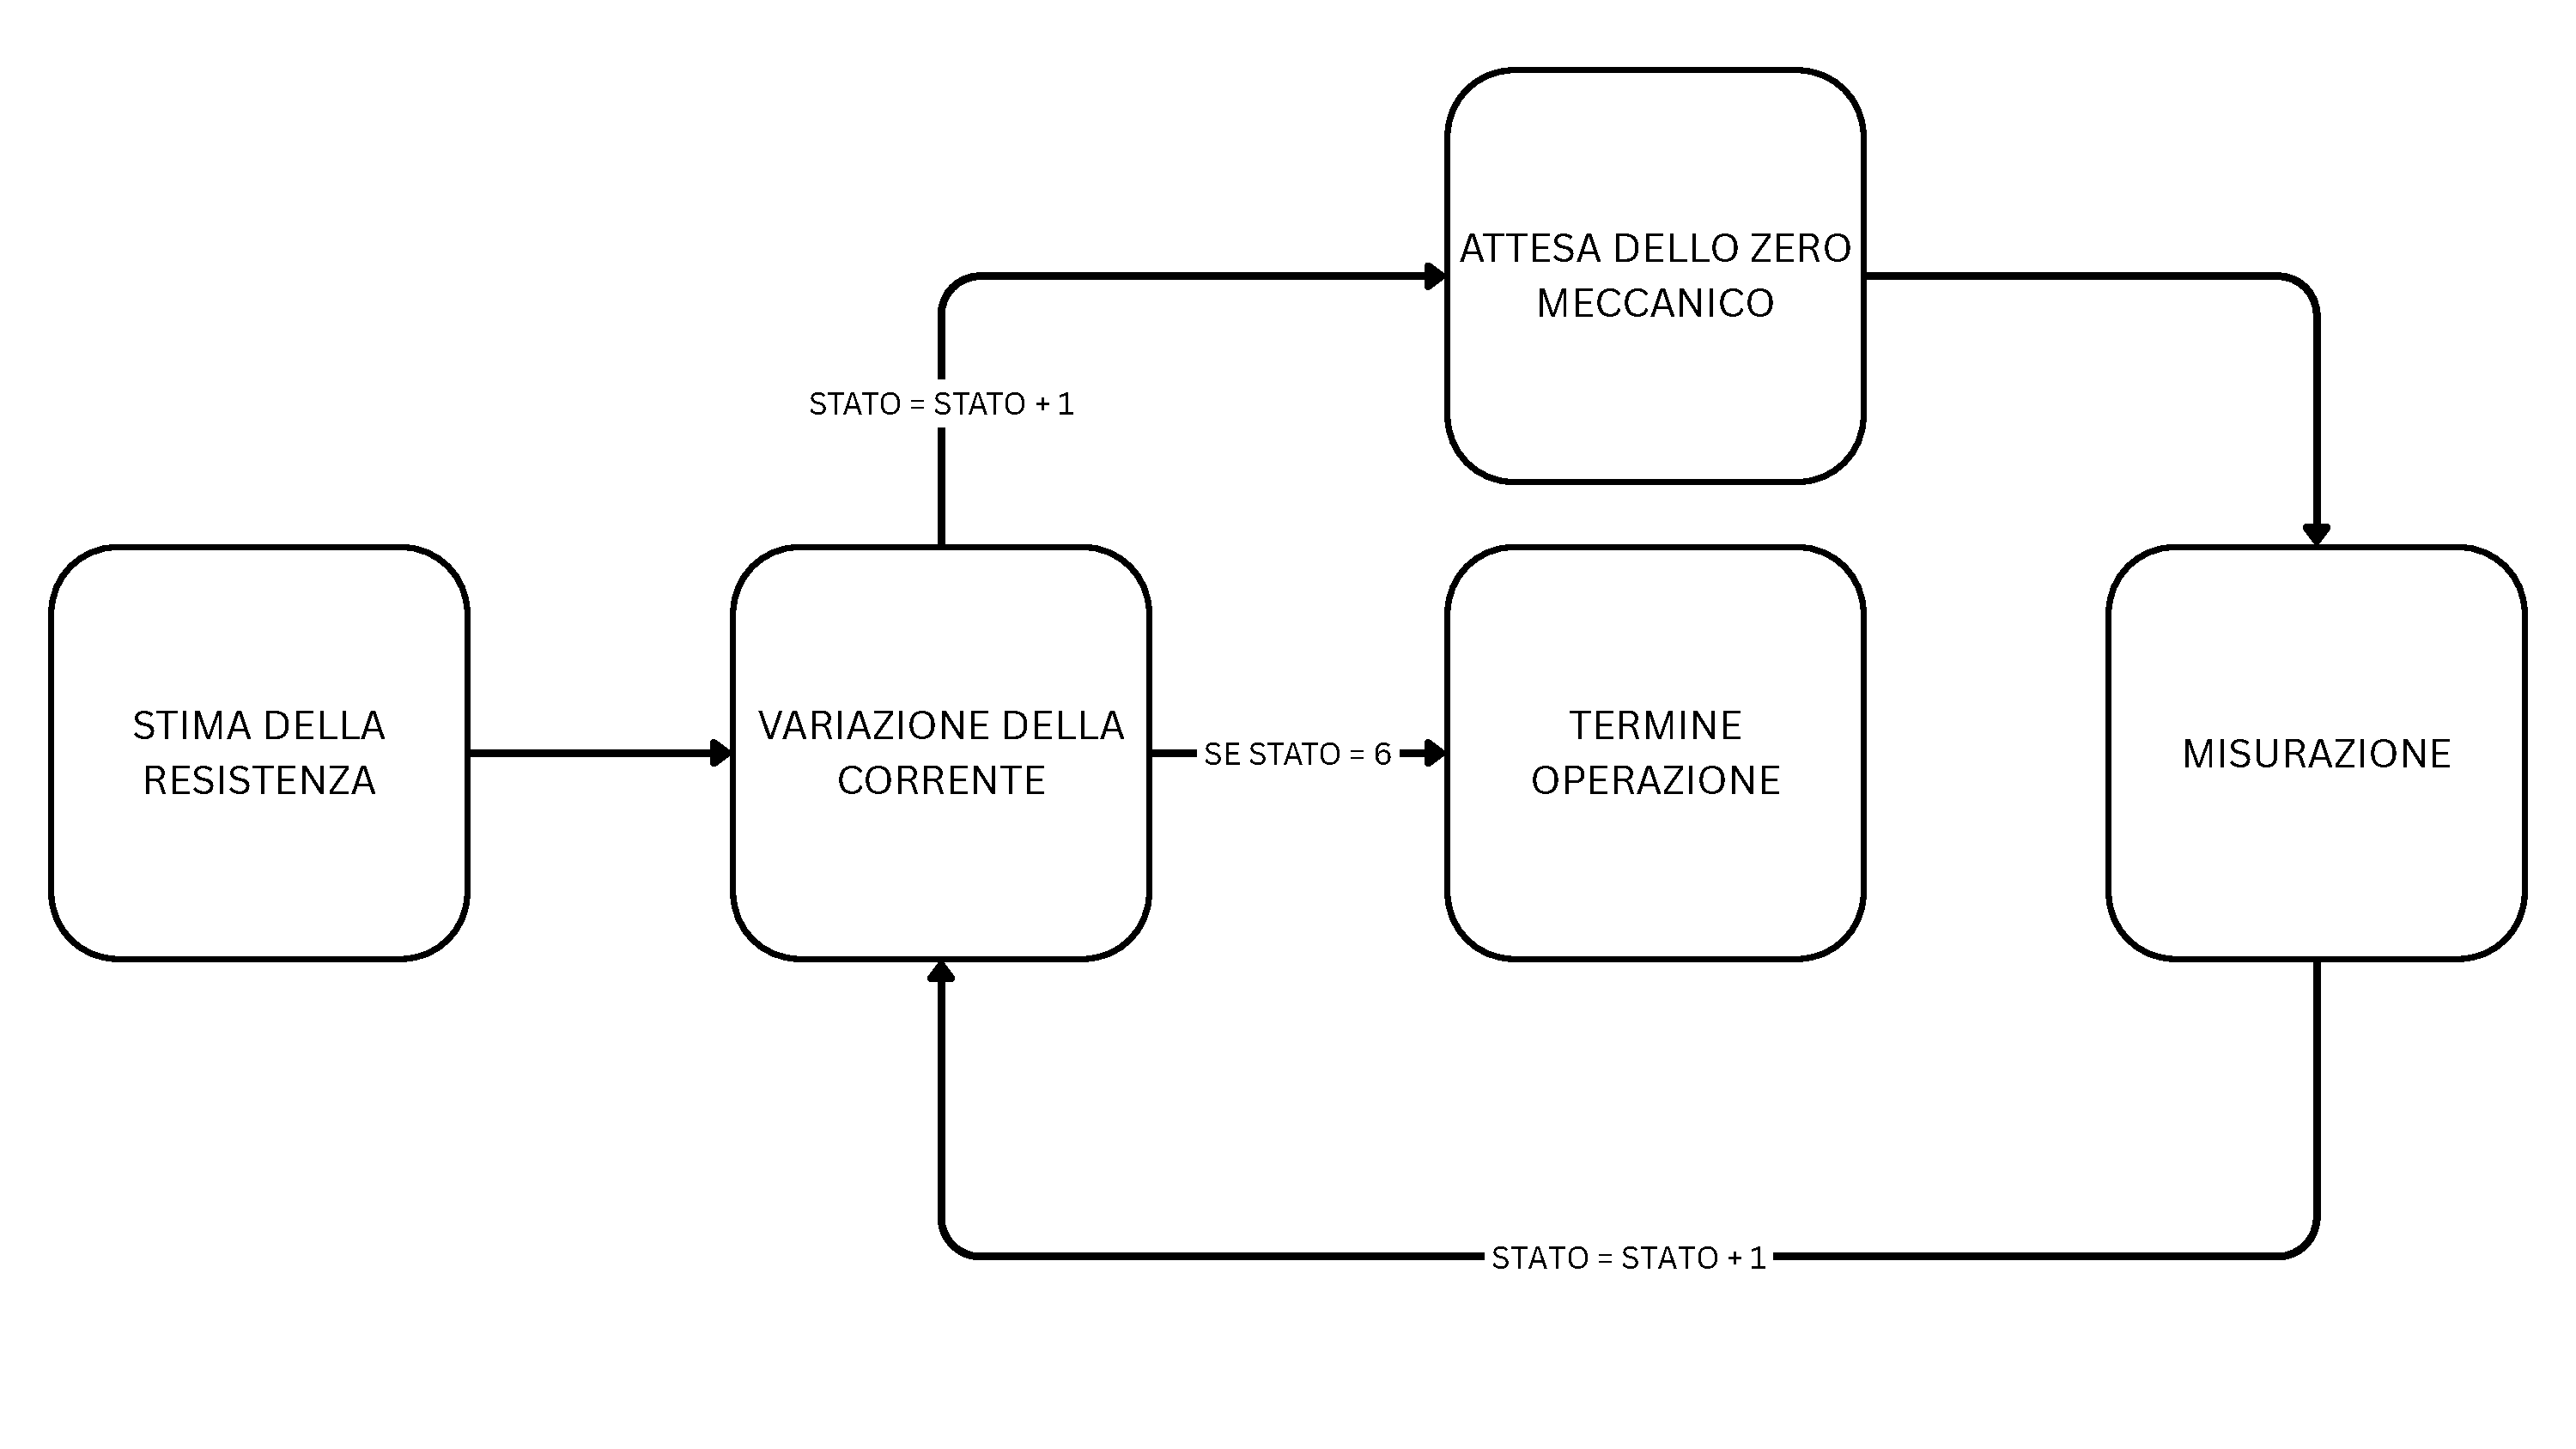
\includegraphics[height=8 cm]{immagini/immagini_motore/flowchart_stati.pdf}
    \caption{Schema della procedura di misurazione.} 
    \label{fig:flowchart_stati}
\end{figure}

\subsection{Fase di stima della resistenza di statore}
Le stime del flusso per ogni coppia di correnti vengono eseguite in successione. Di conseguenza, all'avvio di ogni sessione di raccolta dati, si riscontra una temperatura diversa da quella di partenza e quindi anche una resistenza differente.\\
Per stimare la resistenza, all'inizio di ogni sessione di misurazione viene applicato un segnale di corrente $i_d$ pari a metà della corrente nominale \cite{Gierczynski}. \\
Come nella fase di variazione di corrente, anche in questa fase si raggiunge il valore desiderato tramite una rampa di corrente. Anche in questo caso la pendenza è pari a $2 \ A/s$.\\
La corrente $iq$ viene mantenuta nulla per la durata dell'impulso $id$.\\
Dato che la corrente $iq$ è pari a 0, anche il flusso $\lambda_q$ risulta nullo.\\
In questo modo risulta che:


\begin{equation}
    u_d = R_{s}\cdot i_d
\label{eq:res_iq_null}
\end{equation}
\begin{equation}
    u_q = \omega_{me}\cdot\lambda_d(i_d,i_q,\theta_m)
\end{equation}
Atteso l'esaurimento del transitorio, vengono prelevati 100 campioni di corrente e tensione.\\
Dalla \ref{eq:res_iq_null} si può ricavare una stima della resistenza:
\begin{equation}
\hat{R}_{ph} = \overline{u}_d / \overline{i}_d , 
\end{equation}




\subsection{Fase di variazione di corrente}

Come prima cosa viene verificat loo stato del sistema.
Se il contatore ha raggiunto il valore di 6, significa che il sistema ha completato la procedura di misurazione per un determinato punto di lavoro e deve terminare l'operazione.\\
Inanzitutto si impone i valori di corrente $i_d$ e $i_q$ da raggiungere. Tali valori identificano un punto della griglia nella procedura completa.
I riferimenti di corrente $i_q^*$ e $i_d^*$ variano linearmente fino a raggiungere il valore desiderato. \\
Si è fissata una pendenza della rampa di corrente pari a $2 \ A/s$. Dato che il tempo di campionamento è di $10^{-4}$ s, l'incremento di corrente ad ogni passo di esecuzione è pari a $2\cdot10^{-4}$ A.\\
Una volta che la differenza tra il riferimento di corrente e il valore desiderato è inferiore all' incremento di corrente, il riferimento di corrente viene fissato al valore desiderato.\\ 
Senza questa accortezza, la corrente di riferimento potrebbe non raggiungere il valore desiderato.\\
La scelta della pendenza della rampa è significativa in quanto influenza la durata della procedura di misurazione. Tuttavia, una pendenza troppo elevata può portare a oscillazioni della corrente e quindi a una stima del flusso non corretta.\\
Una volta raggiunto il valore desiderato viene attivato un flag che permette il passaggio allo stato successivo.\\


\subsection{Fase di attesa dello zero meccanico}
Prima di iniziare la fase di misurazione, è necessario attendere che la posizione meccanica del rotore sia pari a 0°.\\
In questo modo, infatti è garantito che tutte le misurazioni vengano eseguite a partire dalla stessa posizione meccanica.\\
Per evitare di iniziare a campionare quando il transitorio di corrente non si è ancora esaurito si è deciso di attendere un tempo di 0.2 s prima di iniziare la fase di misurazione.\\
Se il rotore raggiunge la poszione meccanica di 0° prima che siano trascorsi 0.2 s il sistema attende fino a quando il motore non raggiunge nuovamente tale posizione meccanica e il tempo di attesa è trascorso.\\

\begin{figure}
\centering
    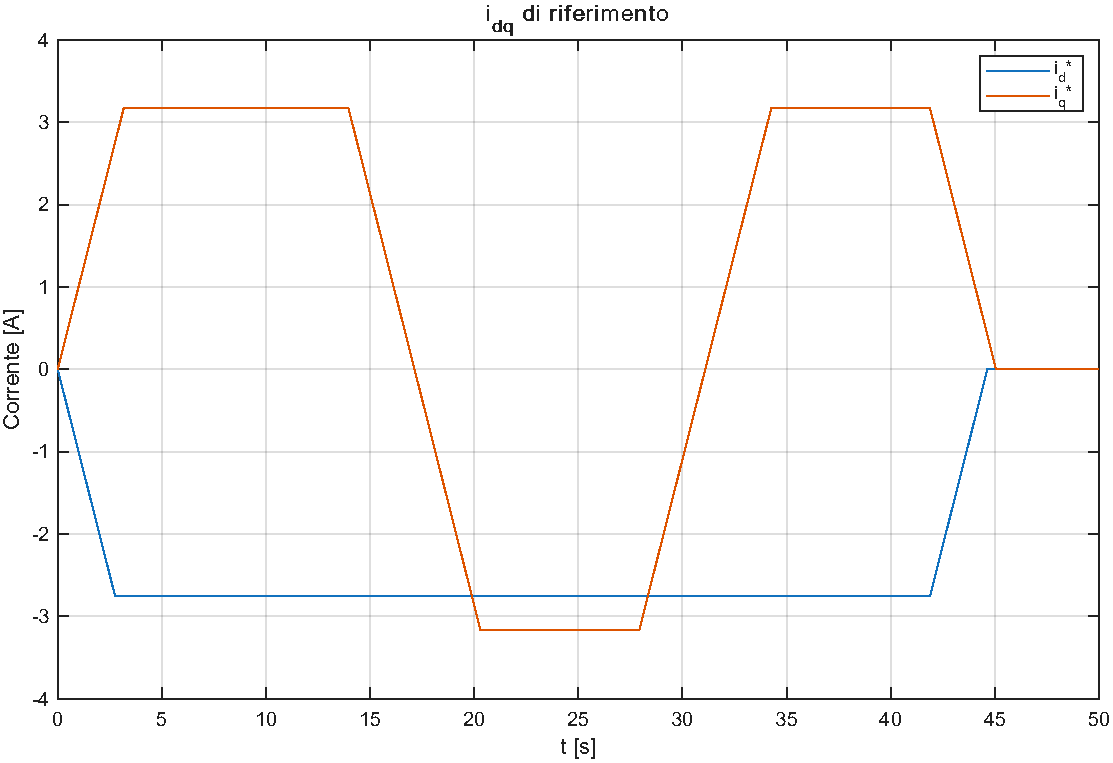
\includegraphics[height=8 cm]{immagini/procedura_misurazione/Curr_ref_proc.pdf}
    \caption{Andamento della corrente di riferimento ( $i_d$ = -2.692, $i_q$ = 3.224 A)}
    \label{fig:Curr_ref_proc}
\end{figure}

\subsection{Fase di misurazione}
In questa fase le misure di corrente e tensione vengono caricate in un vettore di dati.\\
I dati inviati al workspace di MATLAB sono la tensione, la corrente e la poszione meccanica. I dati di corrente e tensione sono espressi secondo il sistema $abc$ e verranno poi trasformati nel sistema $\alpha\beta$.\\
Per attivare il caricamento dei dati nel vettore apposito, viene attivato un flag che abilita il blocco "Enabled Subsystem" di Simulink.\\
La procedura di misurazione termina quando il rotore completa un giro meccanico.\\
A ogni passo di esecuzione, viene calcolata la differenza tra la posizione attuale e quella precedente. Questo valore viene somamto a un contatore che permette di registrare la distanza angolare percorsa dal rotore.\\
Per separare le misurazioni di corrente, posizione e tensione avvenute nelle avrie fasi, al termine di una misurazione viene aggiunto un elemento NaN al del vettore di dati.\\
Una volta che il contatore raggiunge il valore di $360^{\circ}$, il sistema transita allo stato successivo e disabilita il blocco "Enabled Subsystem".\\


\subsection{Conclusione della procedura}

Una volta che il sistema ha effettuato l'ultima misurazione (M2), il sistema transita nuovamente allo stato di variazione di corrente. Il contatore \texttt{stato} ha raggiunto il valore 6, quindi le correnti di target vengono impostate a 0.\\
Dopo che entrambe le correnti hanno raggiunto il valore nullo, la simulazione termina dopo 1 s per attendere l'esaurimento del transitorio.\\
Il blocco \texttt{Stateflow} infine attiva un flag per teminare la simulazione.\\


\subsection{Andamento del segnale di corrente $dq$}
Per realizzare una mappa di flusso precisa, è necessario che, durante la fase di misura, la corrente rimanga il più possibile costante.\\
Si può notare in Figura \ref{fig:Curr_ref_proc_tot_stat} come, a regime, la corrente di statore oscilli intorno al valore di riferimento. Tuttavia, tale oscillazione risulta ininfluente e non incide sulla stima finale.\\
In quanto il flusso magnetico è influenzato dalla posizione, ad alta velocità il controllo risulta complesso. Esso, infatti, risulta affetto da oscillazioni significative che portano a una distorsione del segnale del flusso stimato. Il disturbo sul controllo di corrente è evidente in Figura \ref{fig:Curr_ref_proc_tot_5_rads}, dove la velocità di test imposta è di 5 rad/s.



\begin{figure}
\centering
    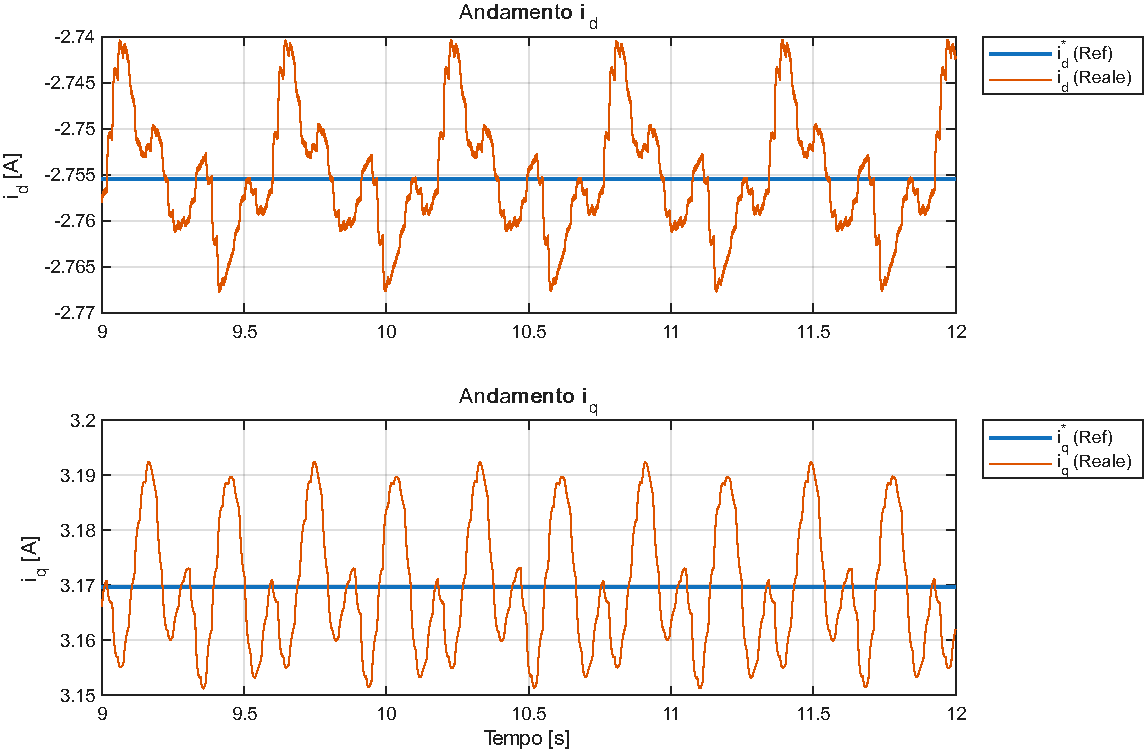
\includegraphics[height=8 cm]{immagini/procedura_misurazione/Curr_ref_proc_tot_stat.pdf}
    \caption{Oscillazione della corrente rispetto al riferimento ( $i_d$ = -2.692, $i_q$ = 3.224 A)}
    \label{fig:Curr_ref_proc_tot_stat}
\end{figure}

\begin{figure}
\centering
    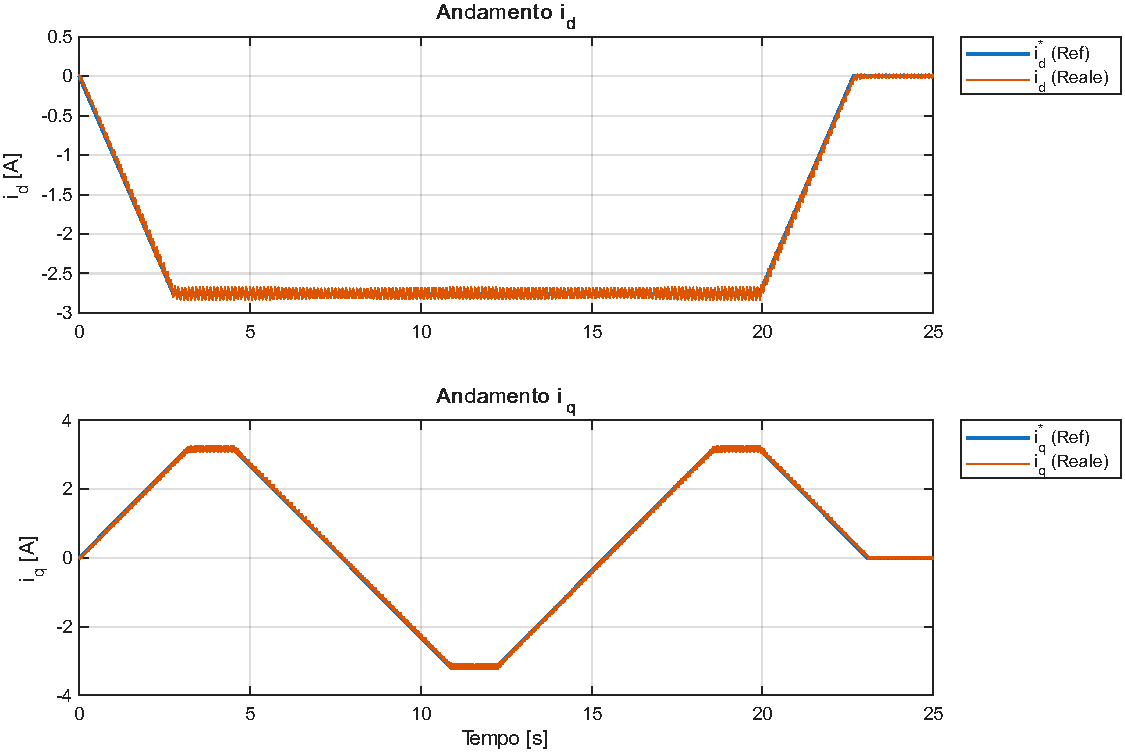
\includegraphics[height=8 cm]{immagini/procedura_misurazione/Curr_ref_proc_tot_5_rads.pdf}
    \caption{Andamento della corrente dq @ $\omega_m = 5\ rad/s$}
    \label{fig:Curr_ref_proc_tot_5_rads}
\end{figure}


 



\section{Procedura di campionamento}
I dati vengono campionati a una frequenza di 10 KHz, la stessa dell'inverter. La risoluzione dei sensori scelta è di $1\ mA$ per il sensore di corrente, $10 \ mV$ per il sensore di tensione e $5.49 \cdot10^{-3}$ gradi per il sensore di posizione.\\
Le grandezze di tensione, corrente e posizione meccanica costituiscono i segnali di ingresso per il blocco Stateflow di MATLAB. In tale blocco viene implementata sia la generazione del vettore di corrente, sia la gestione dei dati da inviarre al workspace di MATLAB.\\
Inizialmente, durante la fase di variazione della corrente e di attesa venivano salvati degli elementi NaN all'interno del vettore di output. Tuttavia, questo aumenta la dimensione del vettore di output.\\
Per ovviare a questo problema, si è deciso di salvare solo i dati della fase di misura, eliminando quelli della fase di variazione della corrente.\\
Per implementare questa proceura si è utilizzato il blocco "Enabled Subsystem" di Simulink.

\section{Elaborazione dati}
L'elaborazione dei dati raccolti avviene tramite un algoritmo MATLAB. Tale algoritmo, come la procedura di misurazione, può essere suddivisa in diverse parti:
\begin{enumerate}
 \item Preparazione dei dati per l'elaborazione tramite l'algoritmo di stima.
 \item Stima del flusso magnetico $\alpha\beta$ tramite l'integrazione della forza contro-elettromotrice.
 \item Trasformazione del flusso magnetico nel sistema di riferimento $dq$.
 \item Applicazione della formula per la stima del flusso magnetico, utilizzando i dati raccolti nelle tre fasi di misurazione (M1,G,M2)
\end{enumerate}

\subsection{Preparazione dei dati}
Per la trasformazione da $\alpha\beta$ a $dq$ è necessario disporre della posizione elettrica $\theta_e$ del rotore.\\
Dato che si tratta di un motore sincrono, tale grandezza è legata alla posizione meccanica del rotore tramite la seguente relazione:

\begin{equation}
\theta_e = {p}\cdot\theta_m
\end{equation}

dove $p$ è il numero di coppie polari del motore.\\
Per applicare la formula di integrazione i vettori di tensione $v_{abc}$ e corrente $i_{abc}$ misurati devono essre espressi secondo il sistema di riferimento $\alpha\beta$.\\ 
Per far ciò, si applica la trasformazione di Clarke sui dati raccolti per ogni fase di misurazione $y$:
\begin{equation}
\boldsymbol{v_{\alpha\beta}}{k} = \frac{2}{3} \cdot 
\begin{bmatrix} 
1 & -\frac{1}{2} & -\frac{1}{2} \\ 
0 & -\frac{\sqrt{3}}{2} & \frac{\sqrt{3}}{2} 
\end{bmatrix} \cdot \boldsymbol{v}_{abc,k}^{y}
\label{eq:eq14}
\end{equation}
\section{Elaborazione dati}
Una volta raccolti i dati essi vengono elaborati tramite un algoritmo \texttt{MATLAB}. Questo algoritmo implementa la procedura illustrata nel Paragrafo \ref{sec:stima_flusso}. I dati vengono quindi espressi secondo il sistema di riferimento $\alpha\beta$ . Si sottrae la componente resistiva alla tensione di Bus per ottenere la componente di forza contro-elettromotrice. 
Si integra la forza contro-elettromotrice e la si somma al valore del flusso all'istante iniziale.\\
A questo punto si esprime il flusso secondo il sistema $dq$. Dato che è necessario esprimere il flusso in funzione della posizione elettrica, i dati vengono riordinati a seconda della posizione elettrica. Nel caso in cui più dati siano associati alla stessa posizione elettrica si esegue una media dei valori di flusso.\\
A questo punto è possibile creare una funzione interpolatrice per confrontare i risultati ottenuti con il flusso reale, derivato dalle mappe dirette.



\subsection{Scelta della velocità meccanica del motore}
È poi necessario scegliere una velocità di rotazione del motore adeguata.\\
Una velocità troppo bassa porta a una maggiore influenza delle perdite nel ferro e nel magnete permanente, compromettendo una corretta stima del flusso. Tuttavia, una velocità elevata rende più difficile misurare il flusso per ogni posizione meccanica del motore. \\Ciò è dovuto al fatto che il tempo di campionamento di 10 KHz permette di misurare la posizione ogni 0.1 ms. Se la velocità è elevata, in tale intervallo di tempo lo spostamento del motore può superare la risoluzione del motore IPM sotto test ($5.493 \cdot 10^{-5} rad$).\\
Per ottenere una mappatura completa del flusso a seconda della posizione in un solo giro meccanico è necessario rispettare il seguente vincolo sulla velocità meccanica del rotore $\omega_M$:
\begin{equation}
\omega_M<\frac{\Delta_M}{T_s}  
\end{equation}
Nel caso del motore di test che abbiamo scelto il vincolo sulla velocità meccanica risulta:
\begin{equation}
\omega_M<0.958\ rad/s)
\end{equation}
\subsection{Trade-off sulla velocità del rotore}
Incrementare la velocità richiede necessariamente una sessione di misura più estesa o, in alternativa, il declassamento del dettaglio della mappatura.
Per esempio si potrebbe decidere di far ruotare il motore a una velocità tale che lo spostamento del motore in un intervallo di campionamento equivalga al doppio della risoluzione angolare ed effettuare due misurazioni. \\
Con questo metodo, è possibile recuperare il dettaglio originario effettuando due acquisizioni sfasate; in tal modo, il tempo complessivo di misura rimarrebbe invariato.\\
Tuttavia, in questo caso, la posizione del rotore in corrispondenza della quale iniziare la misurazione non è più ininfluente. È indispensabile che la seconda misurazione inizi con uno sfasamento di una tacca rispetto alla prima.



\begin{comment}
\subsection{Elaborazione dei dati ottenuti}
Una volta calcolato l'integrale della differenza tra la tensione misurata ai terminali e la tensione resistiva ($V_{\alpha \beta}-R_sI_{\alpha\beta}$), i dati ottenuti vengono filtrati con un filtro passa-alto.\\
L'obiettivo di quest'ultima operazione è:
\begin{itemize}
    \item Eliminare la componente DC: eliminare offset costanti che causerebbero una deriva del segnale.
    \item Riduzione dei fenomeni spuri: attenuare disturbi a bassa frequenza e anomalie di misura.
\end{itemize}

Per progettare il filtro passa-alto si è stata implementata la seguente equazione:

\begin{equation}
    y[k] = \alpha y[k-1] + \alpha (x[k] -x[k-1])
\end{equation}

Il parametro $alpha$ si ottiene a partire dalla frequenza di taglio di un equivalente filtro passa-alto in continua. Tale frequenza di taglio deve essere necessariamente inferiore rispetto alla frequenza della prima armonica del flusso magnetico $d$ e $q$. La fondamentale a di entrambi i flussi è centrata in:
\begin{equation}
    f_0 = \frac{w_m\cdot12}{2\pi} = 1.71\ Hz
\end{equation}
Per rispettare questo vincolo è stata scelta una frequenza di taglio di 1 Hz.
\end{comment}





\cleardoublepage
\chapter{Elaborazione sui dati ottenuti}

\begin{figure}
\centering
    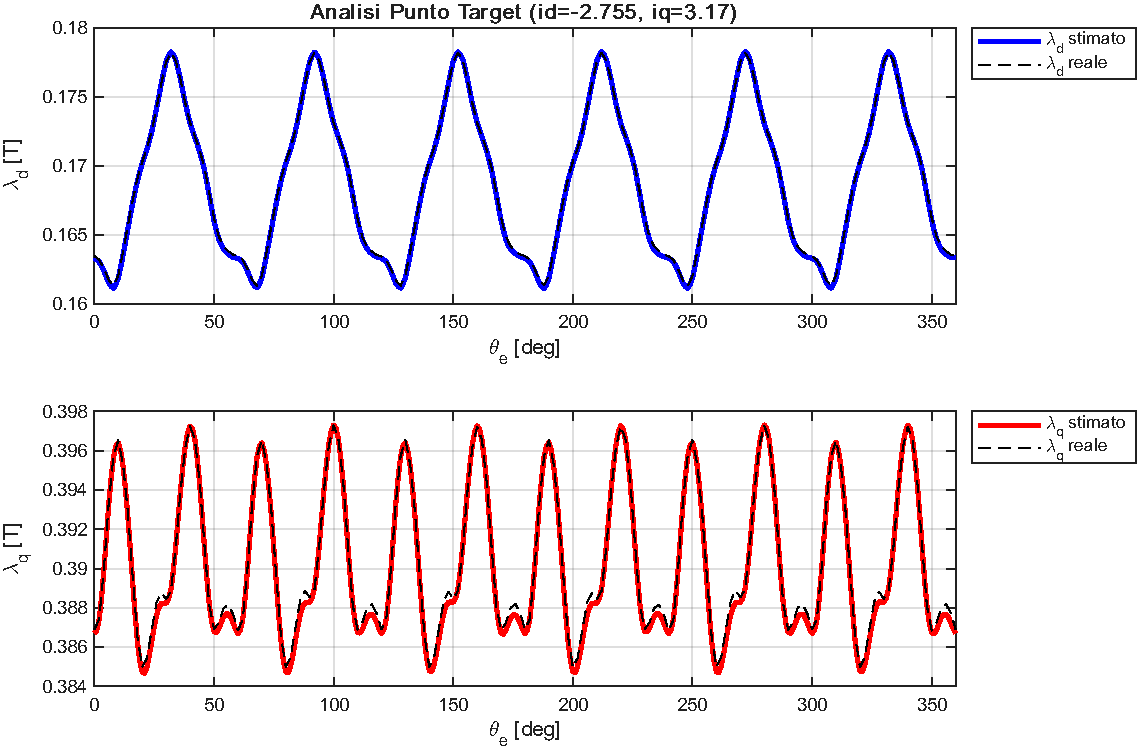
\includegraphics[height=8 cm]{immagini/procedura_misurazione/Confronto_Flussi_PuntoTarget.pdf}
    \caption{Confronto tra il flusso stimato $dq$ e il flusso reale.}
    \label{fig:Flusso_D_vs_Id_ThetaVar_1}
\end{figure}

\section{Analisi dell'errore di stima}
Applicando le formule \ref{eq:flussi_dq2} e \ref{eq:flussi_dq3} è possibile ottenere la stima finale del flusso. Il grafico ottenuto viene riportatoin Figura \ref{fig:Flusso_D_vs_Id_ThetaVar_1}. Come si può notare, nonostante fosse presente un errore nei grafici precedenti  dovuto alla stima della resistenza, questo errore viene in gran parte compensato con la stima finale.\\
Per valutare l'accuratezza della procedura si può stimare l'errore, calcolando la differenza tra $\lambda_d$ reale e stimato (Figura   \ref{fig:Errore_stima_flusso}).
 Per comprendere meglio l'impatto dell'errore sulla stima si può dividere per il valore medio per stimare l'errore percentuale (Figura \ref{fig:Errore_stima_relativo_flusso}).

\begin{figure}
\centering
    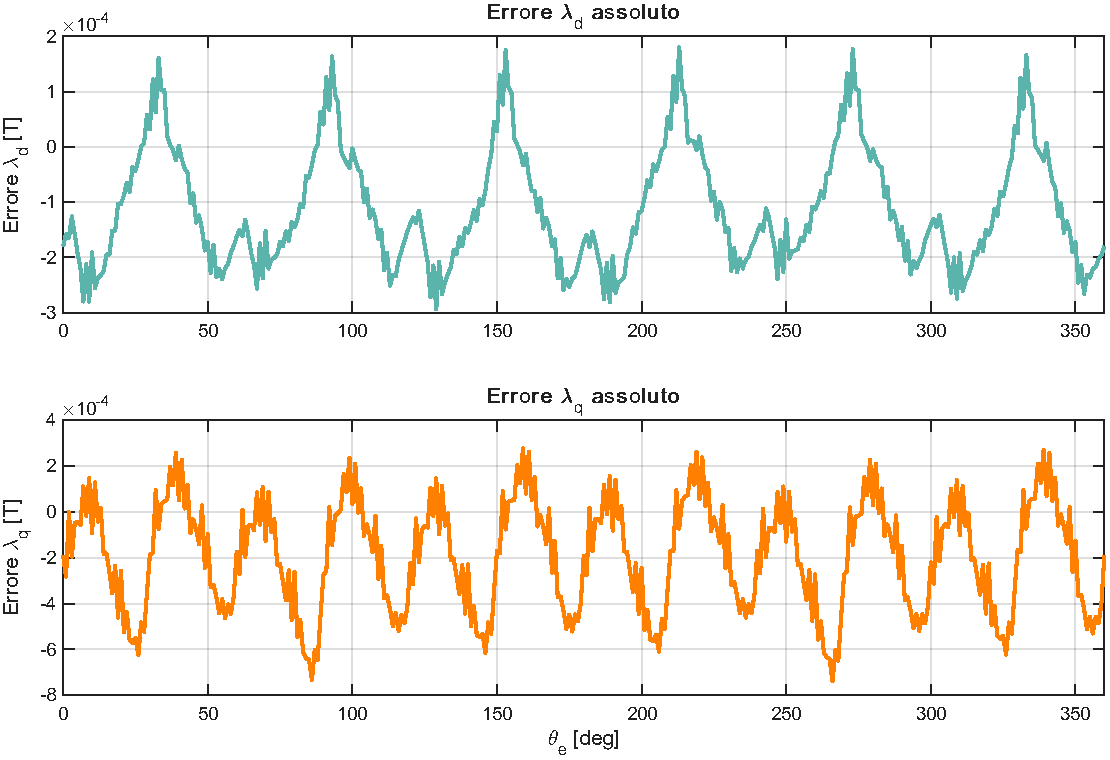
\includegraphics[height=8 cm]{immagini/procedura_misurazione/Errore_stima_flusso.pdf}
    \caption{Differenza tra $\lambda_d$ stimato e reale.}
    \label{fig:Errore_stima_flusso}
\end{figure}


\begin{figure}
\centering
    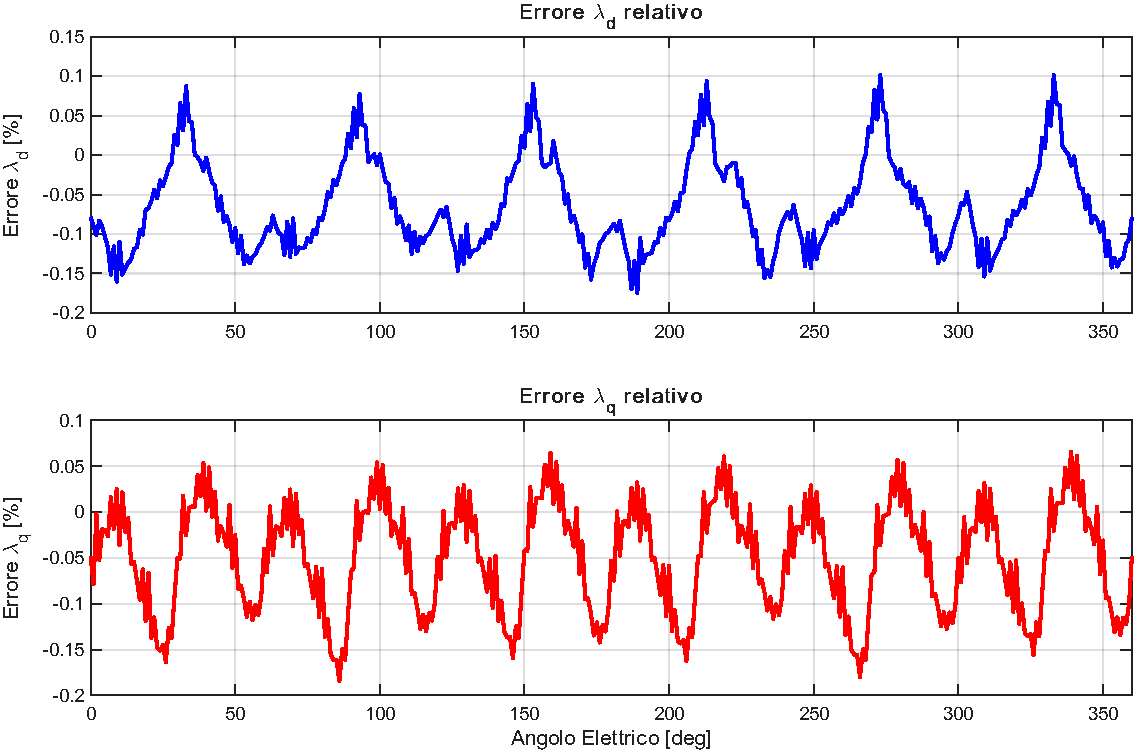
\includegraphics[height=8 cm]{immagini/procedura_misurazione/Errore_stima_relativo_flusso.pdf}
    \caption{Errore percentuale del flusso $\lambda_d$ e $\lambda_q$.}
    \label{fig:Errore_stima_relativo_flusso}
\end{figure}

\section{Introduzione della variazione sulla  resistenza}
Durante la procedura di test, la temperatura del motore aumenta per effetto joule. La variazione della  temperatura comporta una conseguente variazione sulla resistività del rame degli avvolgimenti \cite{Elettrotecnica_1_Principi}.\\ 
La dipendenza della resistività rispetto alla temperatura può essere espressa come segue :
\begin{equation}
    \rho = \rho_0(1+\alpha(T-T_0))
\end{equation}
in cui $T$ è la temperatura effettiva mentre $T_0$ è la temperatura alla quale la resistività è calcolata e $\alpha$ il coefficiente di temperatura caratteristico del materiale.\\
Da tale formula si può ricavare la dipendenza della resistenza dalla temperatura:
\begin{equation}
    R = R_0(1+\alpha(T-T_0))
    \label{eq: res_increase}
\end{equation}
dove $R_0$ è il valore della resistenza alla temperatura $T_0$.\\
Sostituendo i valori standard per il rame e la resistenza statorica del motore sotto test otteniamo:
\begin{equation}
R =  2.726\cdot(1+0.0039\cdot(T-20))  
\end{equation}
Per verificare l'effetto termico, nella simulazione la temperatura cresce linearmente nel tempo. Conseguentemente anche la resistenza aumenta secondo la relazione \ref{eq: res_increase}. \\
Per simulare l'aumento di temperatura del motore dovuta all'effetto joule si è utilizzata una rampa lineare.\\

Si sono provate diverse variazioni di temperatura:
\begin{itemize}
    \item variazione 20°-25°
    \item variazione 20°-30°
\end{itemize}



\begin{figure}
\centering
    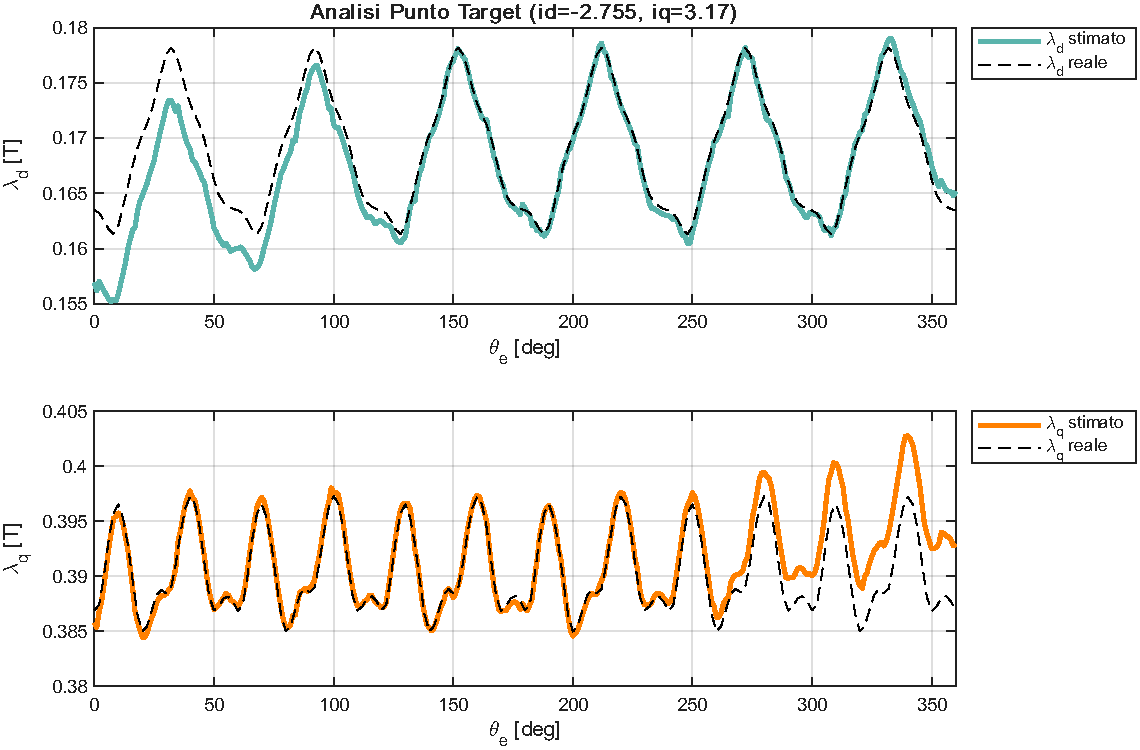
\includegraphics[height=8 cm]{immagini/procedura_misurazione/res_var/Confronto_Flussi_PuntoTarget_res_var.pdf}
    \caption{Stima flusso con resistenza dipendente dalla temperatura.}
    \label{fig:Confronto_Flussi_PuntoTarget_res_var}
\end{figure}

\begin{figure}
\centering
    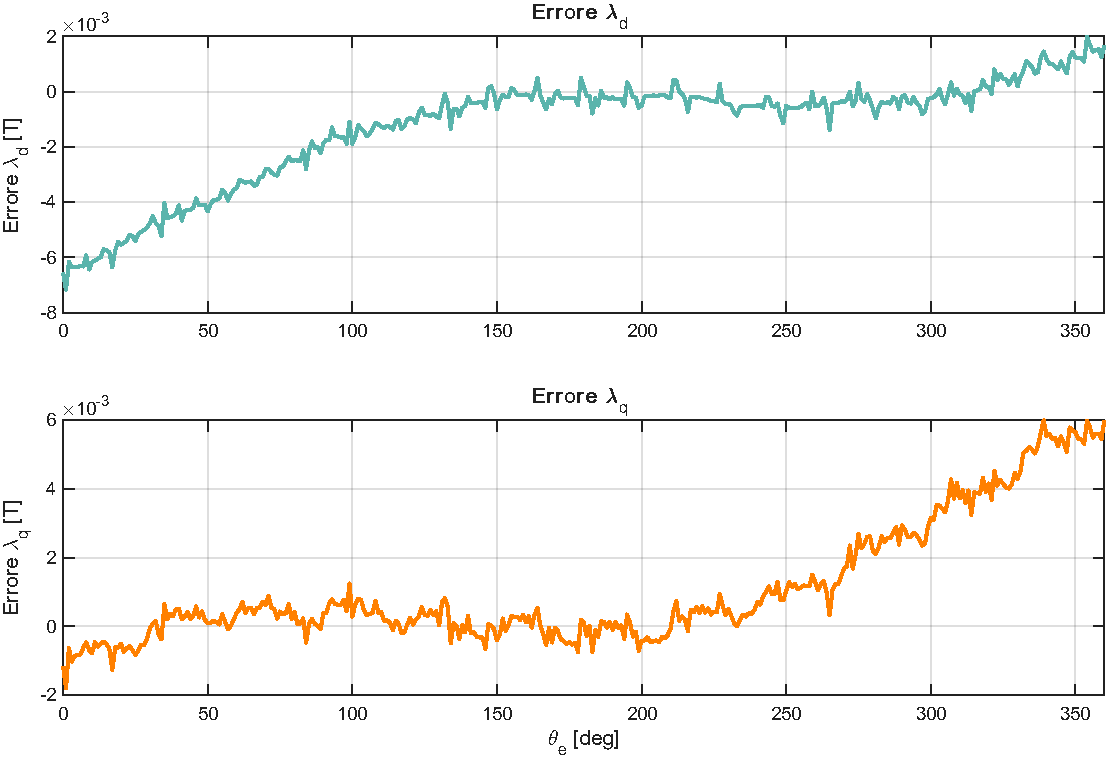
\includegraphics[height=8 cm]{immagini/procedura_misurazione/res_var/Errore_stima_flusso_res_var_500.pdf}
    \caption{Errore di stima del flusso con resistenza variabile.}
    \label{fig:Errore_stima_flusso_res_var_500}
\end{figure}

\subsection{Scelta della posizione iniziale per la raccolta dati}
Inizialmente è stato implementato un algoritmo per la macchina a stati che non prevedeva di iniziare a una specifica posizione angolare.\\
Questo approccio non presenta problemi nel caso in cui il valore della  resistenza statorica rimane costante. Tuttavia, l'introduzione della dipendenza della resistenza dalla temperatura comporta una distorsione molto evidente nella stima del flusso.\\



% ..... COMPLETA

\subsection{Eliminazione dell'errore sul flusso magnetico}
Si osserva come la variazione della resistenza dovuta alla temperatura introduce un errore nella stima (Figura \ref{fig:Confronto_Flussi_PuntoTarget_res_var}).\\
Esaminando l'andamento di questo errore in funzione della posizione si può notare come esso rimane prossimo a zero per la maggior parte dei valori di posizione, ma diverge nel tratto iniziale, nel caso di $\lambda_d$, e finale, nel caso di $\lambda_q$.\\
Per eliminare questo errore di stima i dati della stima di $\lambda_d$ e $\lambda_q$ sono stati post-elaborati utilizzando tre metodi di correzione applicati in successione.
\begin{itemize}
    \item funzione \texttt{polyfit}
    \item fit trigonometrico
    \item correzione degli estremi
\end{itemize}
\subsection{Applicazione della funzione polyfit}
In Figura \ref{fig:Errore_stima_flusso_res_var_500} si può notare come nel primo tratto di $\lambda_d$ e nell'ultimo tratto di $\lambda_q$ sia presente un errore con un andamento circa parabolico.\\ 
Per estrarre questo errore   di stima è stata utilizzata la funzione \texttt{polyfit} di \texttt{MATLAB}. La funzione \texttt{polyfit(x,y,n)} restituisce i coefficienti di un polinomio p(x)  di grado n che costituisce il miglior adattamento per i dati y.\\
Si è scelto 2 come grado del polinomio in quanto l'errore evolve con un andamento circa parabolico.\\
Una volta estratto il polinomio dai dati, viene sottratto per eliminare il trend disatteso.\\
Tuttavia, facendo ciò, viene rimossa anche la componente media. Il valore medio deve così essere nuovamente integrato.\\
Tramite questa procedura di correzione si è ottenuto l'andamento mostrato in Figura \ref{fig:Confronto_Flussi_PuntoTarget_polyfit_500}.



\begin{figure}
\centering
    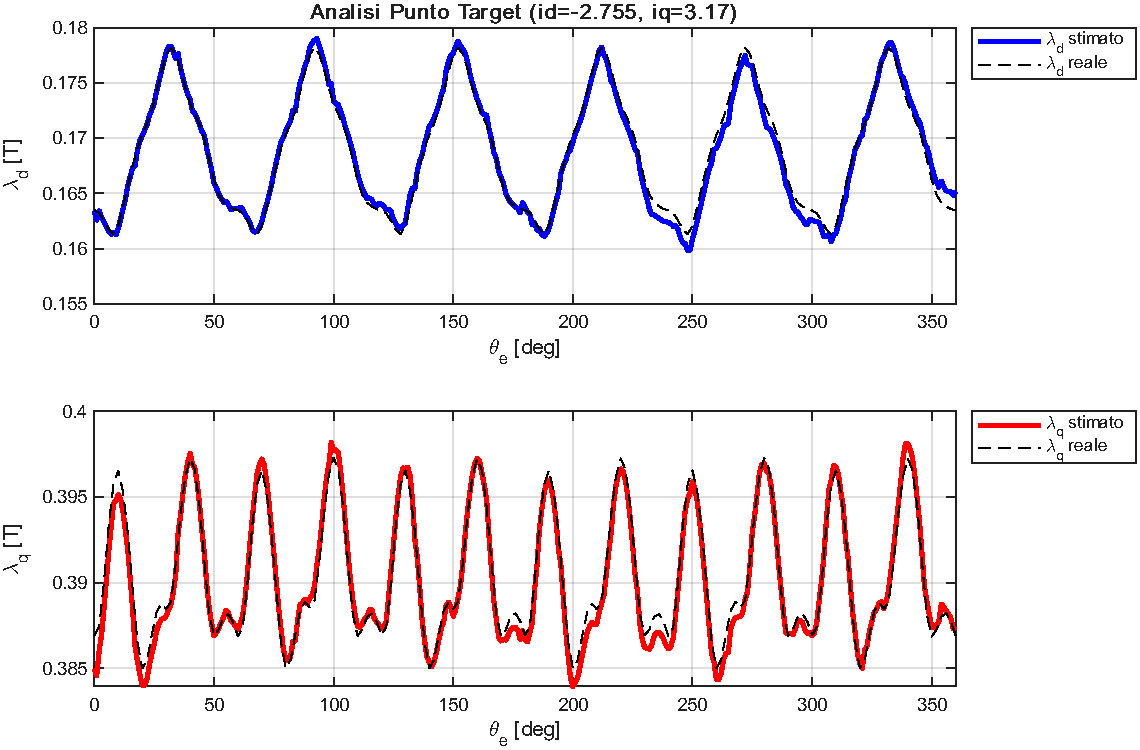
\includegraphics[height=8 cm]{immagini/procedura_misurazione/res_var/Confronto_Flussi_PuntoTarget_polyfit_500.pdf}
    \caption{Confronto dei flussi dopo l'applicazione della funzione \texttt{polyfit}.}
    \label{fig:Confronto_Flussi_PuntoTarget_polyfit_500}
\end{figure}

\begin{figure}
\centering
    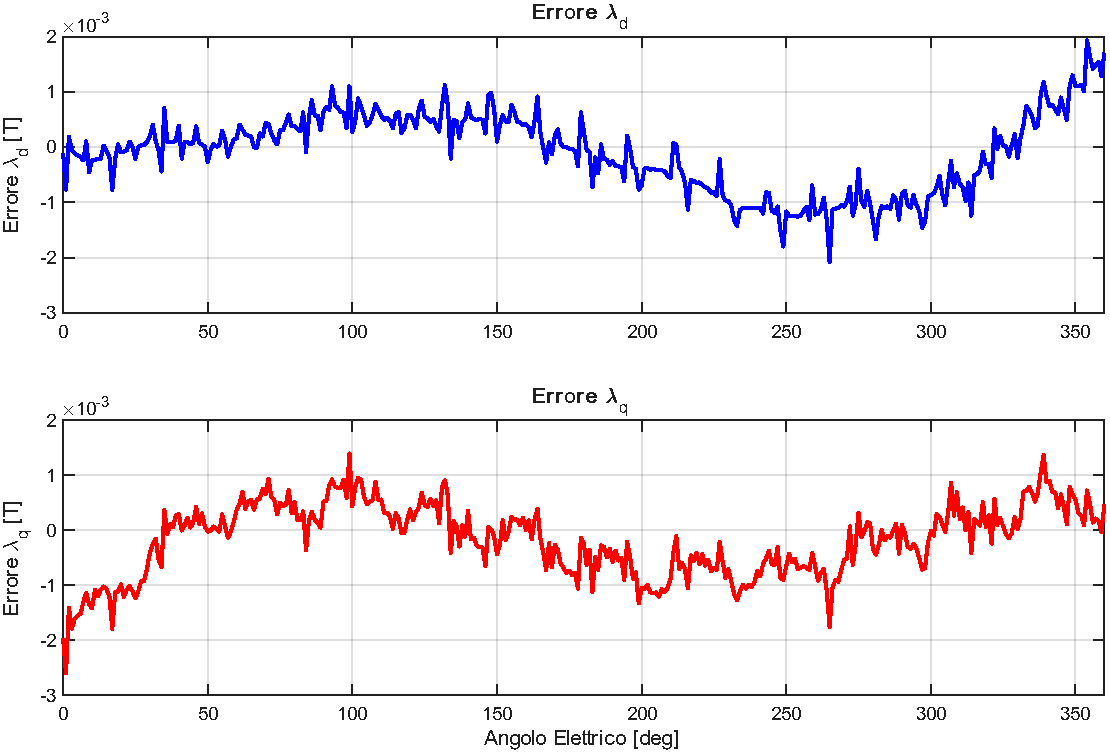
\includegraphics[height=8 cm]{immagini/procedura_misurazione/res_var/Errore_stima_flusso_polyfit_500_.pdf}
    \caption{Errore di stima del flusso dopo l'applicazione della funzione \texttt{polyfit}.}
    \label{fig:Errore_stima_flusso_polyfit_500}
\end{figure}

\subsection{Fit trigonometrico}
Si può notare come sia presente ancora un errore di stima nel tratto finale, sebbene l'estrazione del polinomio abbia migliorato l'accuratezza della stima (Figure \ref{fig:Confronto_Flussi_PuntoTarget_polyfit_500}).  Analizzando la Figura \ref{fig:Errore_stima_flusso_polyfit_500} si osserva come l'errore abbia un andamento simile a quello di una funzione trigonometrica. Tramite un metodo ai minimi quadrati si è quindi estratta la sinusoide che approssima meglio i dati.\\ Come fatto in precedenza si è poi sottratto questa forma d'onda ai dati. \\Il risultato ottenuto è riportato in Figura \ref{fig:Confronto_Flussi_PuntoTarget_armonico_500}.


\begin{figure}
\centering
    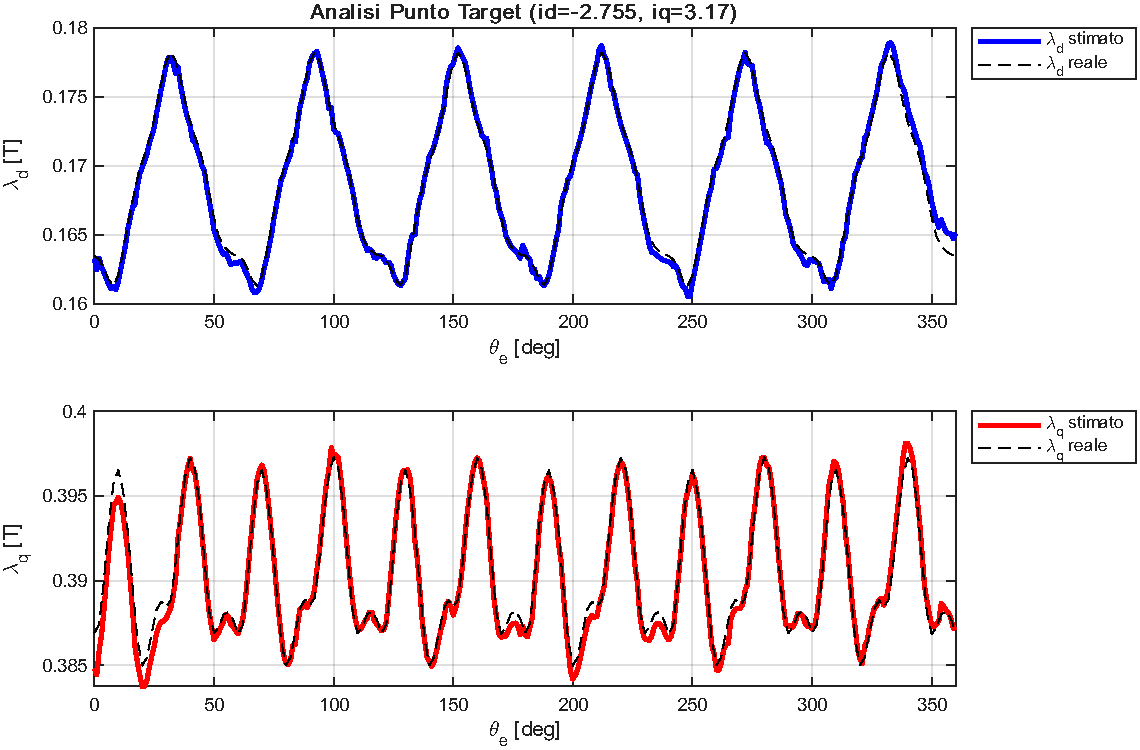
\includegraphics[height=8 cm]{immagini/procedura_misurazione/res_var/Confronto_Flussi_PuntoTarget_armonico_500.pdf}
    \caption{Confronto dei flussi dopo il fitting trigonometrico.}
    \label{fig:Confronto_Flussi_PuntoTarget_armonico_500}
\end{figure}

\subsection{Correzione degli estremi}
Il flusso a 0° deve coincidere necessariamente con il flusso a 360°. Per ovviare a questo problema è stata implementata una correzione usando una curva smooth-step. I risultati sono riportati in Figura \ref{fig:Confronto_Flussi_PuntoTarget_coda_500}.
\begin{figure}
\centering
    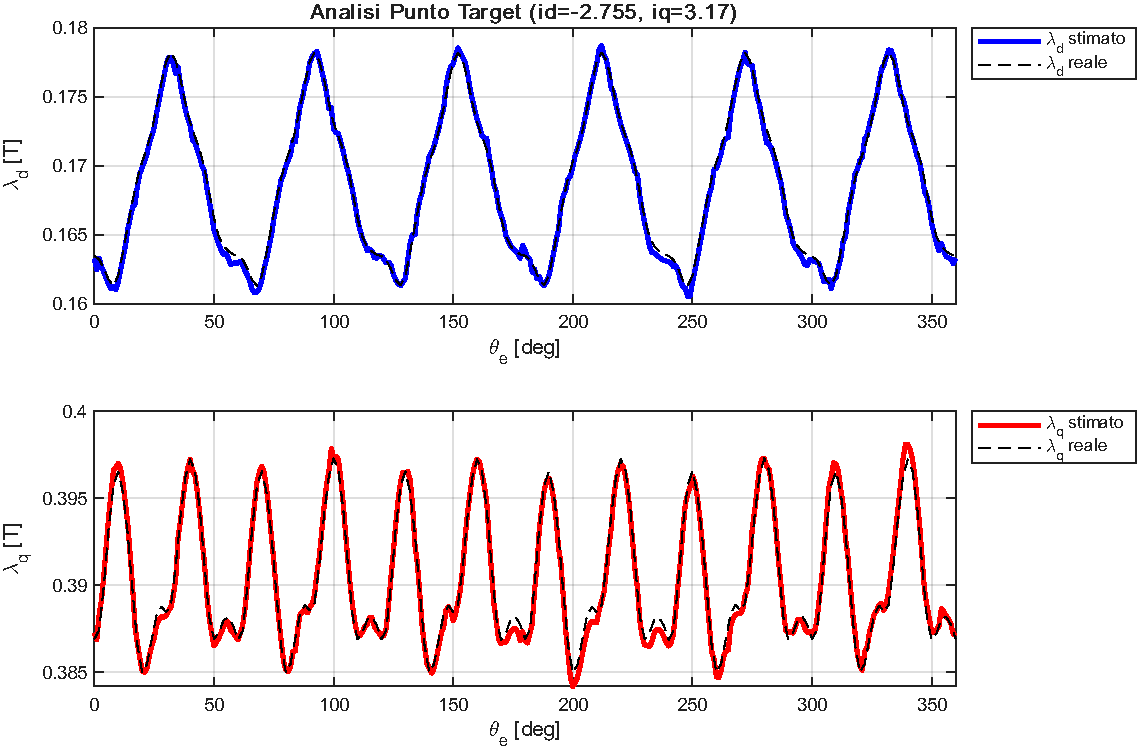
\includegraphics[height=8 cm]{immagini/procedura_misurazione/res_var/Confronto_Flussi_PuntoTarget_coda_500.pdf}
    \caption{Confronto dei flussi dopo la correzione degli estremi.}
    \label{fig:Confronto_Flussi_PuntoTarget_coda_500}
\end{figure}

\subsection{Stima del flusso con range di temperatura 20°-25°}
La stima del flusso nel range 20°-25° risulta accurata. Per validare la procedura, si è stimato il flusso rispetto a 8 punti lungo la curva MTPA.

\begin{table}
    \centering

    \footnotesize

    \bf{Errore di stima su $\lambda_d$}

    \vspace{0.2cm}
    
    \renewcommand{\arraystretch}{1.3}
    \begin{tabular}{
    >{\centering\arraybackslash}m{2.5 cm}
    >{\centering\arraybackslash}m{2.5 cm}
    >{\centering\arraybackslash}m{2.5 cm}
    >{\centering\arraybackslash}m{2.5 cm}
    >{\centering\arraybackslash}m{2.5 cm}
    }
    \arrayrulecolor{black}\toprule
    $\bm{i_d}$ [A]&$\bm{i_q}$ [A]&\textbf{RMSE [T]} &\textbf{Errore medio [\%]} &\textbf{Errore massimo [\%]}\\
    \arrayrulecolor{GRIG}\midrule
        0 & 0
        & $1.42\cdot10^{-4}$
        & 0.06 & 0.13
        \\
    \arrayrulecolor{GRIG}\midrule
        -0.17& 0.57
        & $9.2\cdot10^{-5}$
        & 0.04
        & 0.17
        \\
    \arrayrulecolor{GRIG}\midrule
        
        -0.5& 1.09
        & $1.49\cdot10^{-4}$
        &0.09&0.33
        \\
    \arrayrulecolor{GRIG}\midrule
        
        -0.85& 1.59
        & $2.41\cdot10^{-4}$
        &0.12&0.34
        \\
    \arrayrulecolor{GRIG}\midrule
        
        -1.3& 2.02
        & $2.95\cdot10^{-4}$
        &0.15&0.45
        \\
    \arrayrulecolor{GRIG}\midrule
        
        -1.69& 2.47
        & $3.4\cdot10^{-4}$
        &0.18&0.52
        \\
    \arrayrulecolor{GRIG}\midrule
        
        -2.08& 2.94
        & $3.99\cdot10^{-4}$
        &0.22&0.75
        \\
    \arrayrulecolor{GRIG}\midrule
        
        -2.76& 2.17
        & $3.94\cdot10^{-4}$
        &0.23&0.8
        \\
    \arrayrulecolor{black}\bottomrule
    
    \end{tabular} 
    \caption{Valore dell'errore di stima per punto operativo.}
    \label{tab:Tabella_errore_stima_d}   
\end{table}



\begin{table}
    \centering

    \footnotesize

    \bf{Errore di stima su $\lambda_q$}

    \vspace{0.2cm}
    
    \renewcommand{\arraystretch}{1.3}
    \begin{tabular}{
    >{\centering\arraybackslash}m{2.5 cm}
    >{\centering\arraybackslash}m{2.5 cm}
    >{\centering\arraybackslash}m{2.5 cm}
    >{\centering\arraybackslash}m{2.5 cm}
    >{\centering\arraybackslash}m{2.5 cm}
    }
    \arrayrulecolor{black}\toprule
    $\bm{i_d}$ [A]&$\bm{i_q}$ [A]&\textbf{RMSE [T]} &\textbf{Errore medio [\%]} &\textbf{Errore massimo [\%]}\\
    \arrayrulecolor{GRIG}\midrule
        0 & 0
        & $1.42\cdot10^{-4}$
        & 0.06 & 0.13
        \\
    \arrayrulecolor{GRIG}\midrule
        -0.17& 0.57
        & $9.2\cdot10^{-5}$
        & 0.04
        & 0.17
        \\
    \arrayrulecolor{GRIG}\midrule
        
        -0.5& 1.09
        & $1.49\cdot10^{-4}$
        &0.09&0.33
        \\
    \arrayrulecolor{GRIG}\midrule
        
        -0.85& 1.59
        & $2.41\cdot10^{-4}$
        &0.12&0.34
        \\
    \arrayrulecolor{GRIG}\midrule
        
        -1.3& 2.02
        & $2.95\cdot10^{-4}$
        &0.15&0.45
        \\
    \arrayrulecolor{GRIG}\midrule
        
        -1.69& 2.47
        & $3.4\cdot10^{-4}$
        &0.18&0.52
        \\
    \arrayrulecolor{GRIG}\midrule
        
        -2.08& 2.94
        & $3.99\cdot10^{-4}$
        &0.22&0.75
        \\
    \arrayrulecolor{GRIG}\midrule
        
        -2.76& 2.17
        & $3.94\cdot10^{-4}$
        &0.23&0.8
        \\
    \arrayrulecolor{black}\bottomrule
    
    \end{tabular} 
    \caption{Valore dell'errore di stima per punto operativo.}
    \label{tab:Tabella_errore_stima_q}   
\end{table}





\section{Implementazione dell'algoritmo di stima multiplo}
infine risulta necessario iterare la procedura di stima per ogni coppia di correnti della griglia.\\
I risultati finali vengono salvati all'interno di una mappa.

\begin{comment}
Si è verificato quindi la stima del flusso introducendo questo fenomeno ( Figura \ref{fig:Confronto_Flussi_PuntoTarget_Res}).

\begin{figure}[H]
\centering
    
\includegraphics[height=8 cm]{immagini/flusso_concatenato/Confronto_Flussi_PuntoTarget_Res.pdf}
    \caption{Confronto tra il flusso stimato $dq$ e il flusso reale con variazione resistiva.}
    \label{fig:Confronto_Flussi_PuntoTarget_Res}
\end{figure}

\end{comment}
\begin{comment}
\section{Creazione modello utilizzando le induttanze differenziali}
Si può implementare il modello fisico del motore utilizzando le induttanze differenziali.\\
Dalle equazioni elettriche del motore si ottiene che:

\begin{equation}
\begin{dcases}
    \frac{d\lambda_d}{dt} =u_d- Ri_d+\omega_{me}\lambda_q\\
    \frac{d\lambda_q}{dt} =u_q -Ri_q-\omega_{me}\lambda_d
\end{dcases}
\label{eq:equazioni_elettriche}
\end{equation}

Sostituendo l'espressione delle derivate del flusso ottenute precedentemente (\ref{eq:induttanze_diff_elet}) nelle equazioni \ref{eq:equazioni_elettriche}, si ottiene che:

\begin{equation}
\begin{dcases}
    \frac{di_d}{dt} =\frac{1}{l_d}[ u_d- Ri_d+\omega_{me}\lambda_q-l_{dq}\frac{di_q}{dt}-l_{d\theta}\omega_m]\\
    \frac{di_q}{dt} =\frac{1}{l_q}[ u_q- Ri_q-\omega_{me}\lambda_q-l_{qd}\frac{di_q}{dt}-l_{q\theta}\omega_m]
\end{dcases}
\label{eq:equazioni_elettriche2}
\end{equation}

Le induttanze differenziali possono essere calcolate applicando la funzione "gradient" di MATLAB.\\
Tuttavia, si è notato come questo approccio porti a un maggiore disturbo sulle correnti  $i_d$ e $i_q$.
Ciò si traduce in un errore di stima con la procedura di stima illustrata nel Paragrafo \ref{sec:stima_flusso}.
\end{comment}

\cleardoublepage

\printbibliography[heading=bibintoc]

\end{document}